\section{Results}
\label{sec:results}

In this section we present the results obtained by following the analysis path in Section~\ref{sec:analysis}, in terms of  plots of likelihood ratios $L_p / L_{max}$ as a function of each parameter of interest.  Further details on this ratio as a  measure can be found in the Appendix.  

Plots of the likelihood ratio $L_p/L_{max}$ are shown for the 19 input pMSSM parameters in Figures~\ref{fig:LRwcms_msq} to~\ref{fig:LRwcms_tbmu}.  Similarly Figures~\ref{fig:LRwcms_sq} to~\ref{fig:LRwcms_Higgs} show the likelihood ratio for the physical sparticle masses.  The relations between the scalar SUSY breaking mass parameters with the physical scalar masses as well as the gaugino mass parameters with the physical gaugino masses should be noted.  The colored and shaded histograms in each plot depict the likelihood ratio before and after the inclusion of CMS results, respectively.  We observe that the CMS results indeed introduce a variation in the likelihood ratios, where the variation is more enhanced for some parameters/masses and milder for others.  

We see that all squark/slepton mass parameters and all squark/slepton masses shift upwards systematically after the addition of CMS results.  The gaugino mass parameter $M_3$ and the gluino mass also move up simultaneously due to the constrains coming from the di-jet $\alpha_T$ analysis.  An important aspect to note is that no significant change is observed in the distribution for the mass of $\tilde{\chi}^0_1$, which is the lightest supersymmetric particle (LSP), since neither a stringent $E^T_{miss}$ cut nor any other technique dedicated to constraining the $\tilde{\chi}^0_1$ mass were imposed in the analyses considered.  We owe our ability to observe this effect to the freedom offered by the pMSSM parameterization, in which neutralino/chargino masses are allowed to vary independently from the gluino mass.  Had the interpretation been done using CMSSM, we would be influenced by the strict gaugino mass relationship described in Section~\ref{sec:motivation}, and the $\tilde{\chi}^0_1$ mass would be forced to move upwards in correlation along with the gluino mass.

Figure~\ref{fig:LRwcms_omg} shows $L_p/L_{max}$ for the dark matter relic density calculated using {\tt micrOMEGAs 2.4}~\cite{Belanger:2006is} assuming $\tilde{\chi}^0_1$ is the LSP and the dark matter candidate.  It must be noted that Berger {\it et al.} imposed the WMAP upper limit $\Omega_{\tilde{\chi}^0_1}h^2 \le 0.1210$ as a constraint on the points.  Information from CMS does modify the distribution, however the effect is not sufficient to impose a concrete constraint on $\Omega_{\tilde{\chi}^0_1}h^2$.  This is of course related to the result on $\chi^0_1$ mass.

Finally Figures~\ref{fig:LRwcms_EWobs_s1} and~\ref{fig:LRwcms_EWobs_s2} show distributions for low energy observables as predicted by pMSSM, calculated by {\tt micrOMEGAs 2.4} and {\tt Superiso 2.7}~\cite{Mahmoudi:2008tp}.  We again note that the constraints based on experimental measurements for a subset of these observables were taken into account while selecting the pMSSM points by Berger {\it et al.}.  Similar to the case for the relic density, the 2010 CMS measurements do not yet allow us to constrain these observables further.  However, the prospect of making statements on the predictions for low energy observables in the presence of more data and diverse analysis channels stands out as a strong motivation in favor of interpreting the data within the framework of supersymmetry.

The results we have presented here, with only 35 pb$^{-1}$ of CMS data, show that even with modest amount of data, we are able to start making inferences of a general nature about supersymmetry 
%on a sufficiently generic and well-motivated construction of supersymmetry.  
Therefore we anticipate that at least with an order of magnitude more data, the approach we have developed will allow us to make definitive statements about a broad class of supersymmetric models.  
This is only the starting point that has opened up a vast amount of investigation.  We will develop this study further by considering the following:

\begin{itemize}
\item An improved treatment of the constraints from the EW observables.  We shall replace the box-like likelihood of Berger {\it et al} by a well-defined likelihood function.
\item A significant increase in the sample of pMSSM points 
\item Inclusion of a wider range of final states
\item The construction of a more quantitative treatment of the bounds on the pMSSM parameter space.
\end{itemize}


\begin{figure}[htbp]
\begin{center}
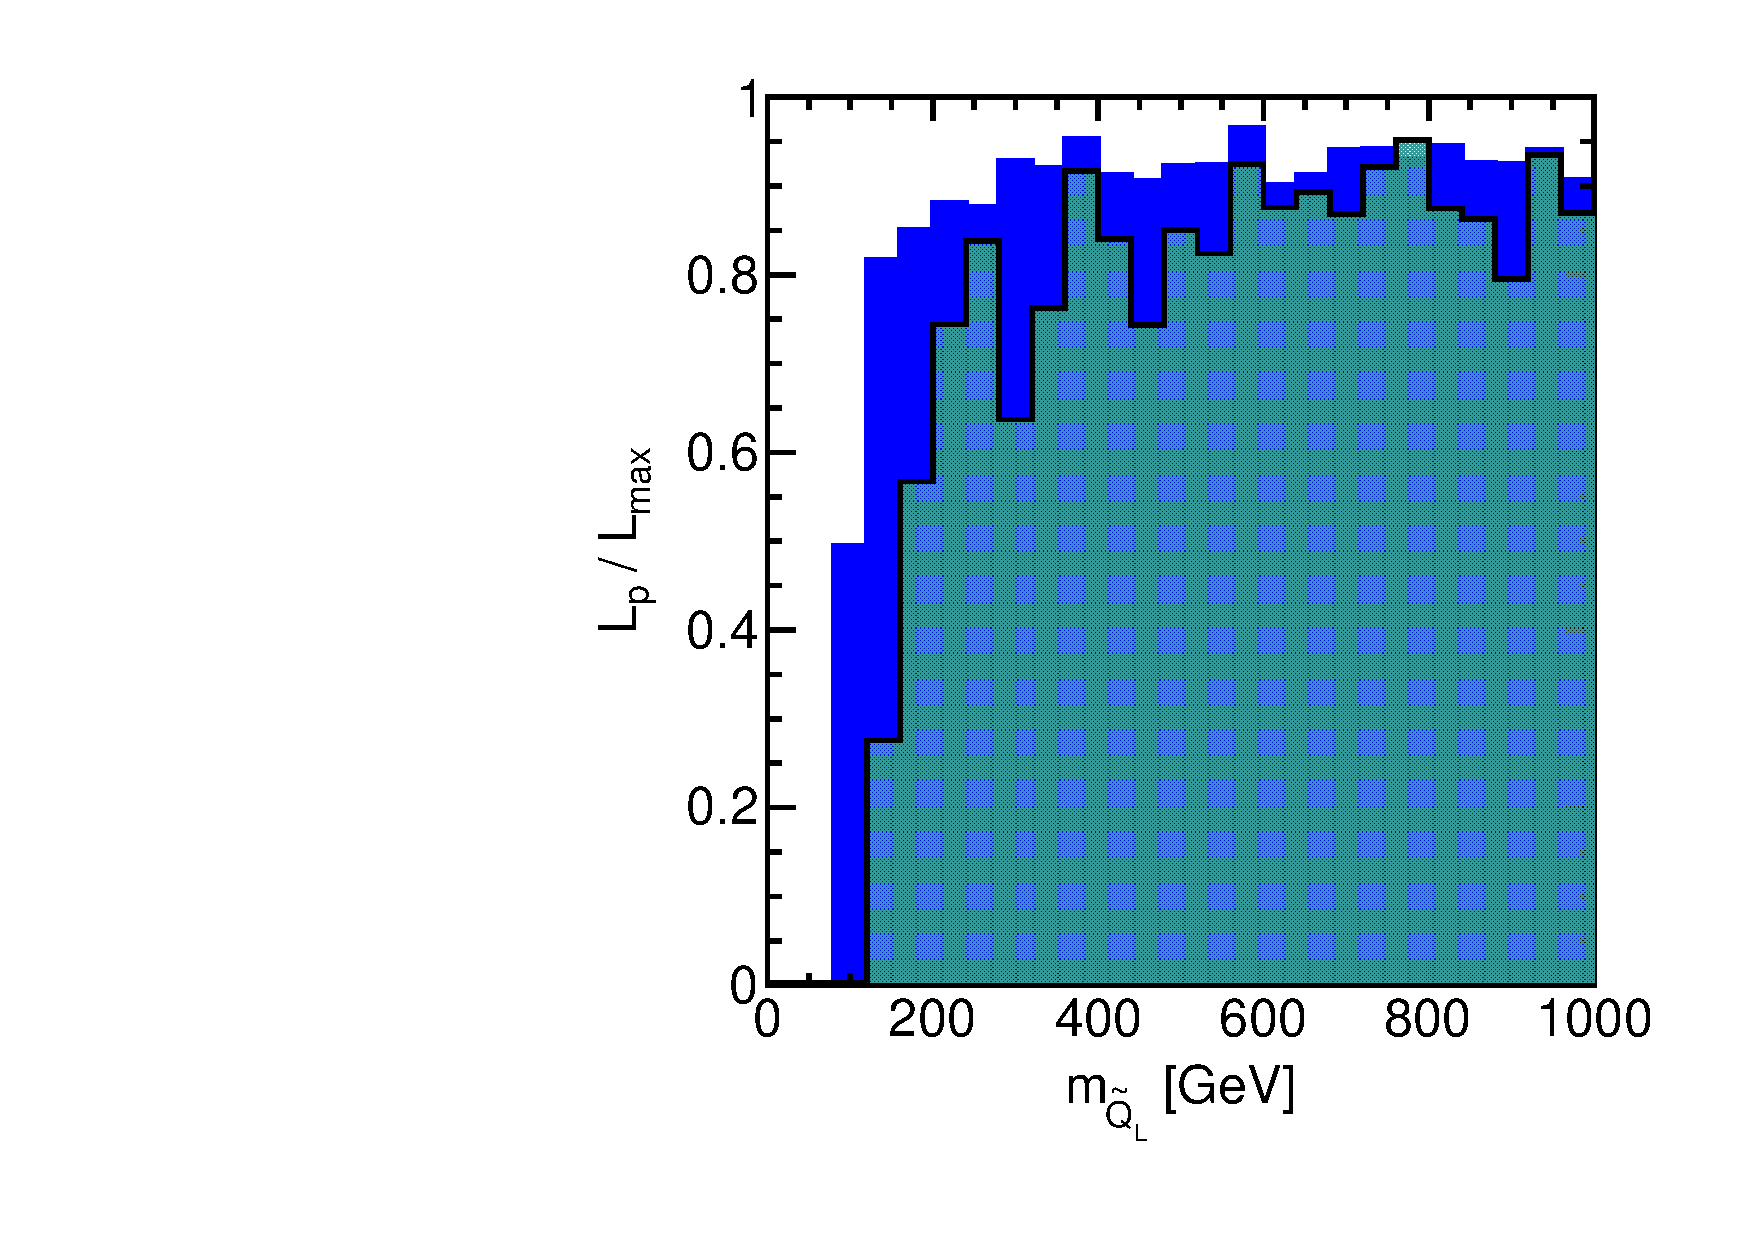
\includegraphics[height=5.5cm]{figs/fig_m_Q_L.pdf} 
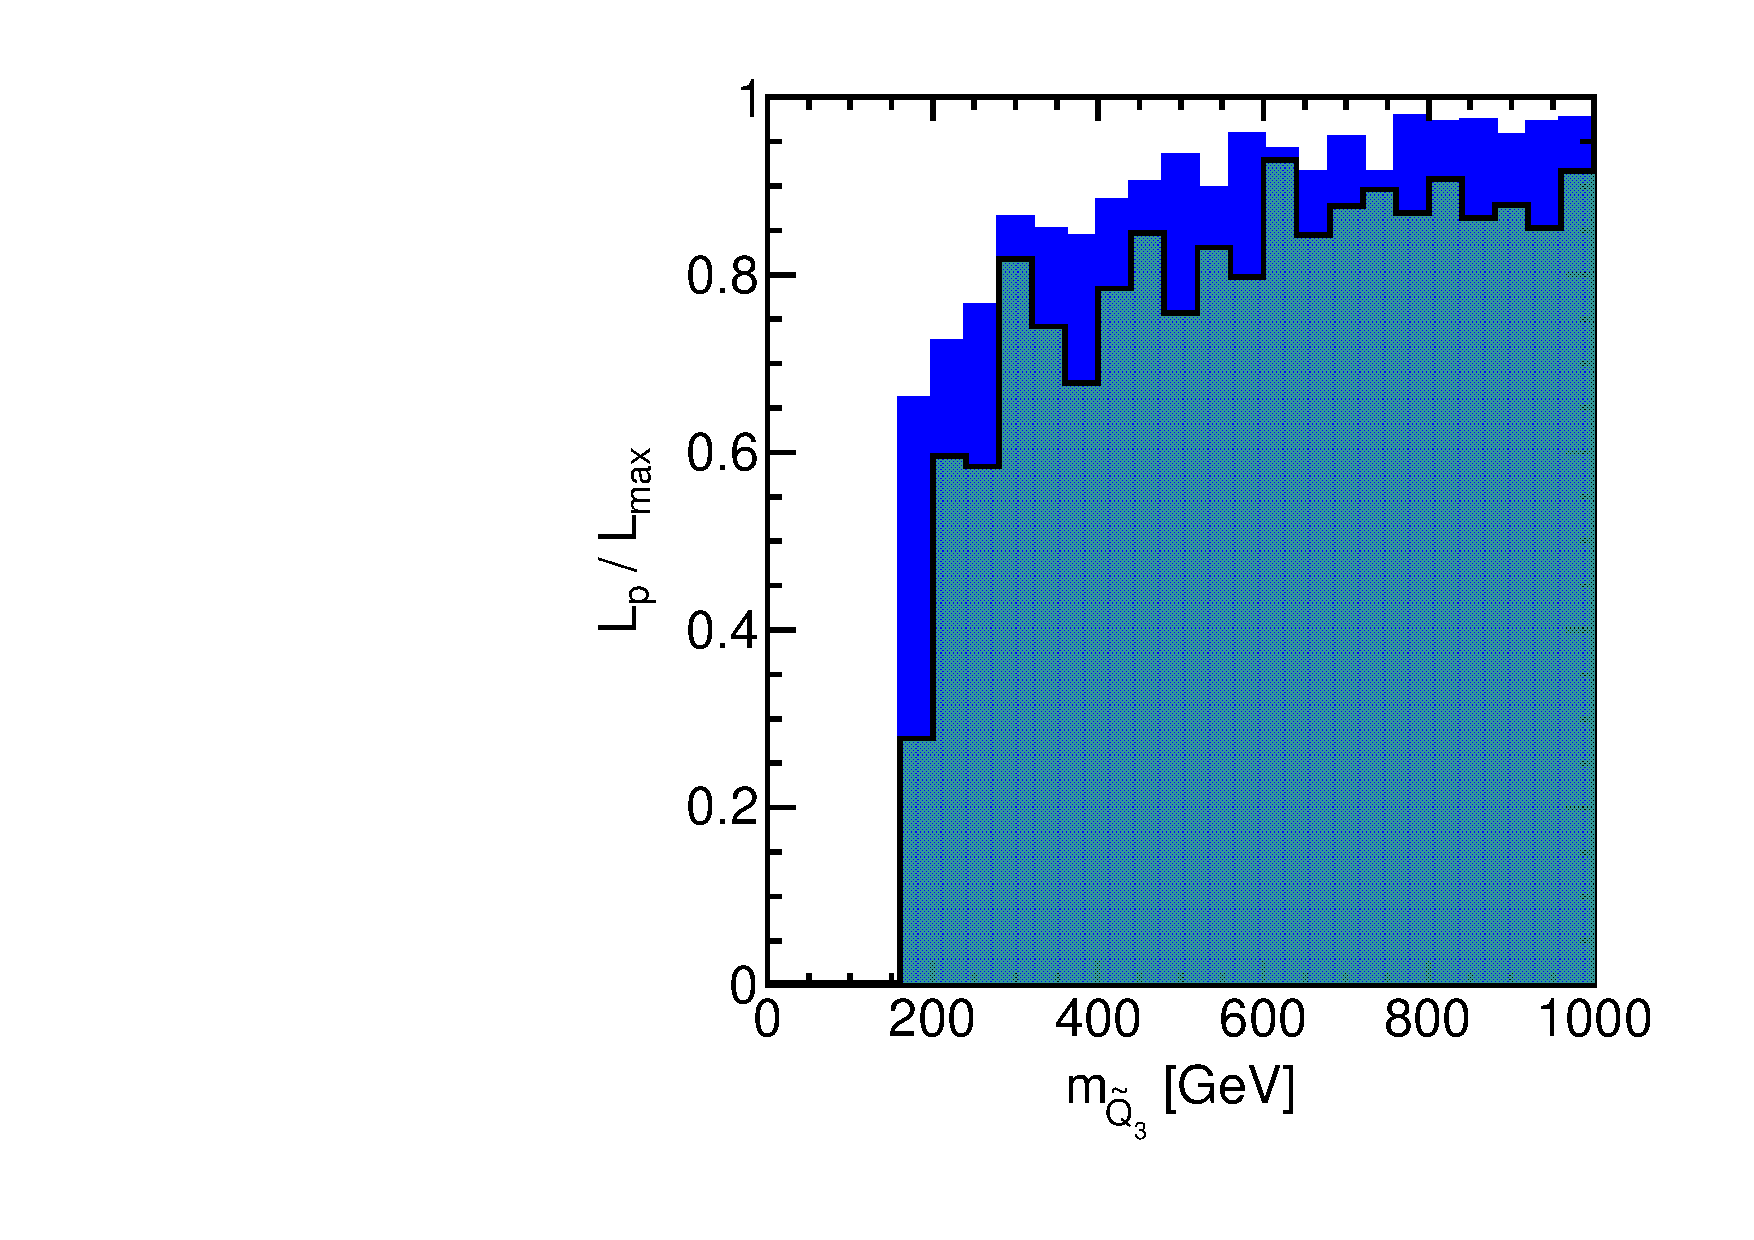
\includegraphics[height=5.5cm]{figs/fig_m_Q_3.pdf} \\
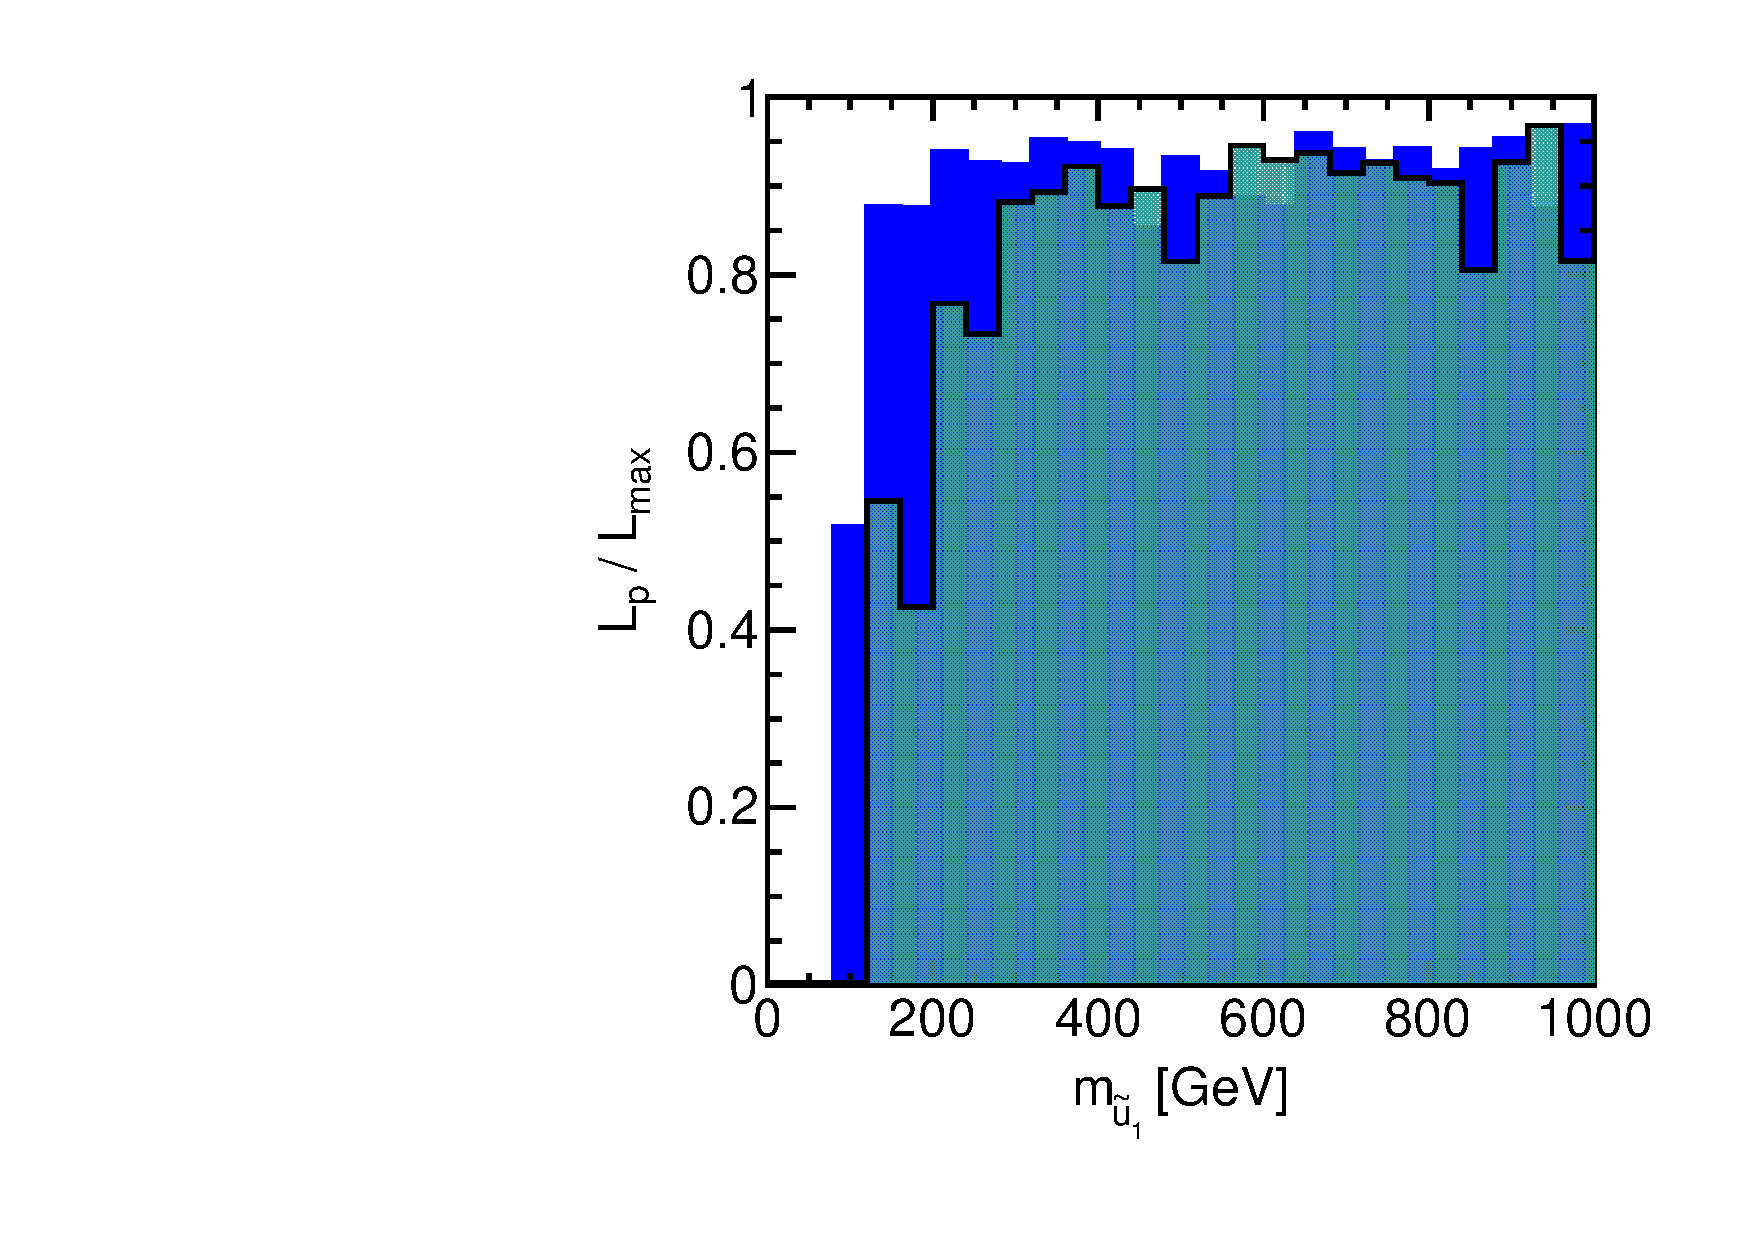
\includegraphics[height=5.5cm]{figs/fig_m_u_1.pdf}
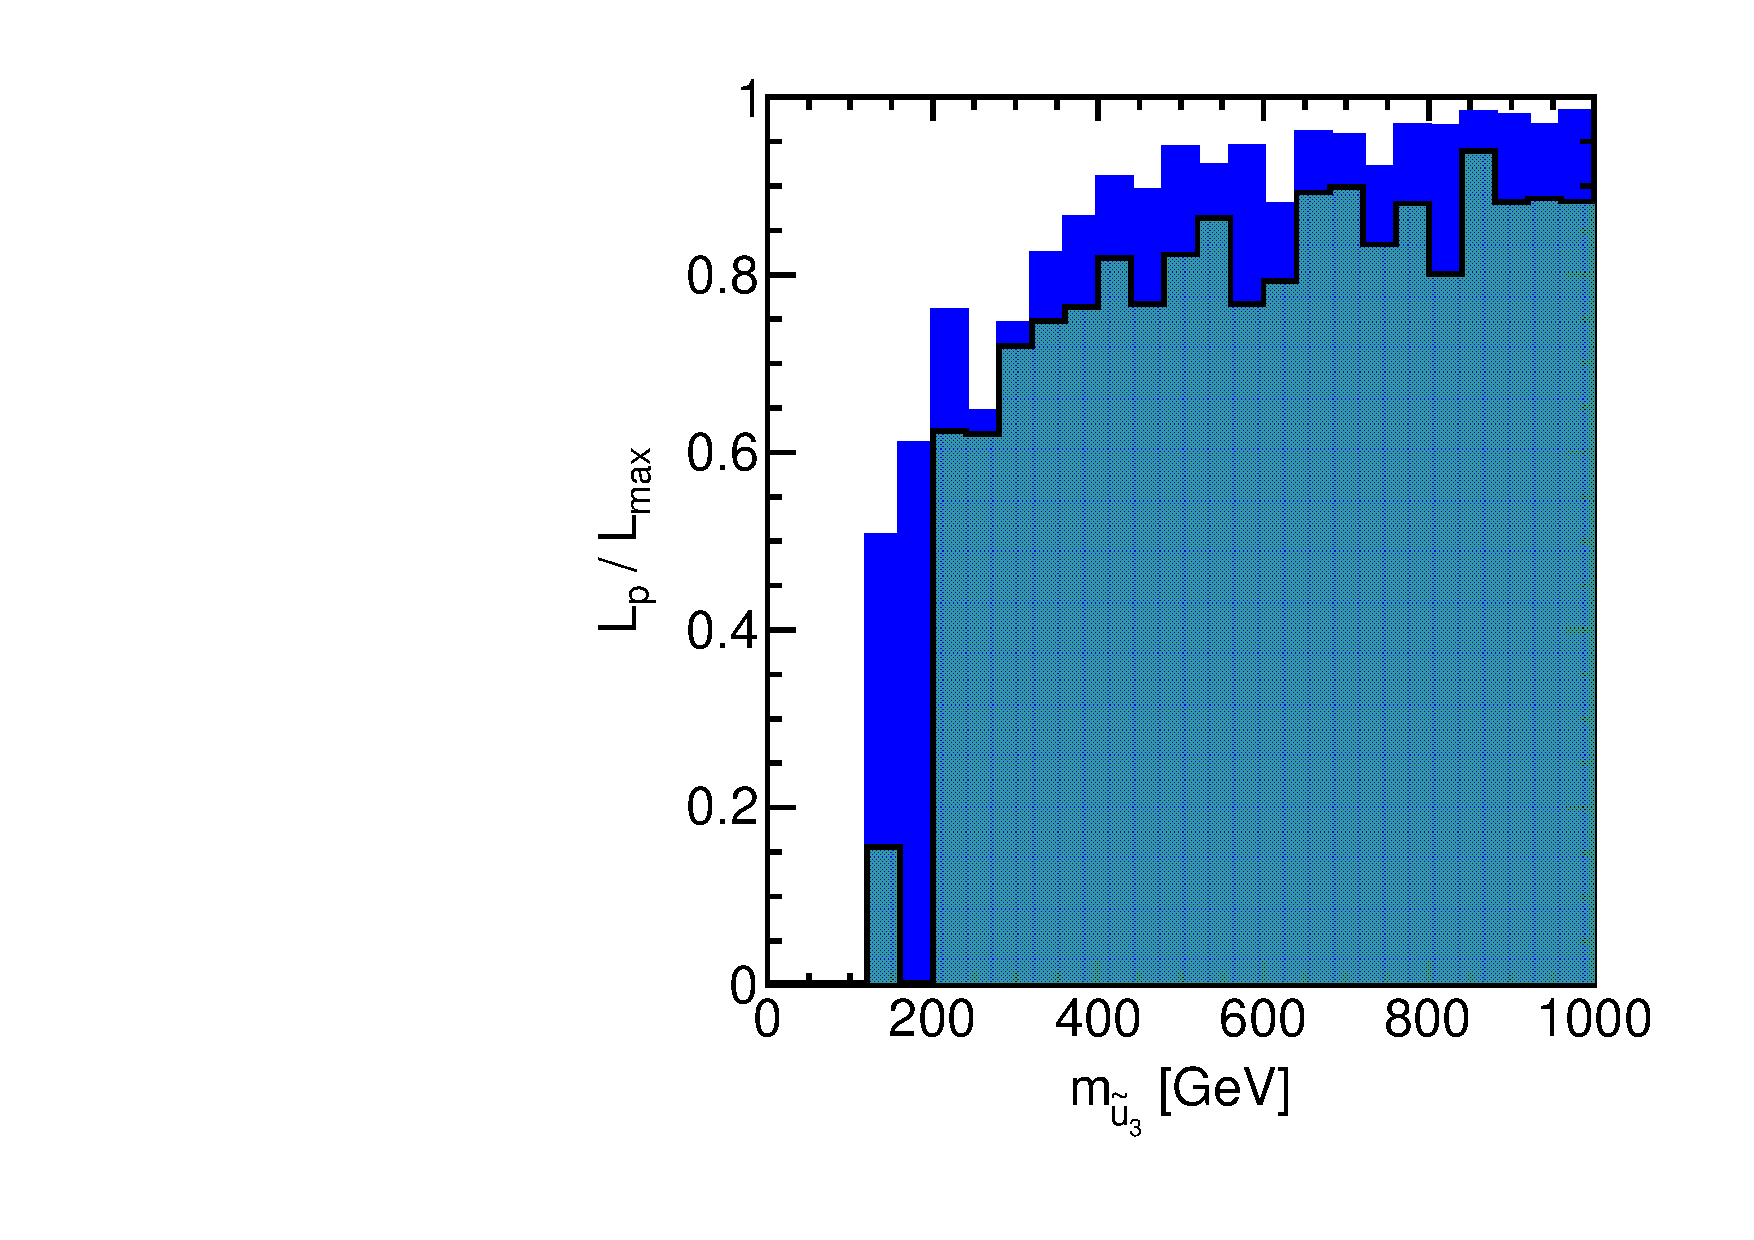
\includegraphics[height=5.5cm]{figs/fig_m_u_3.pdf} \\
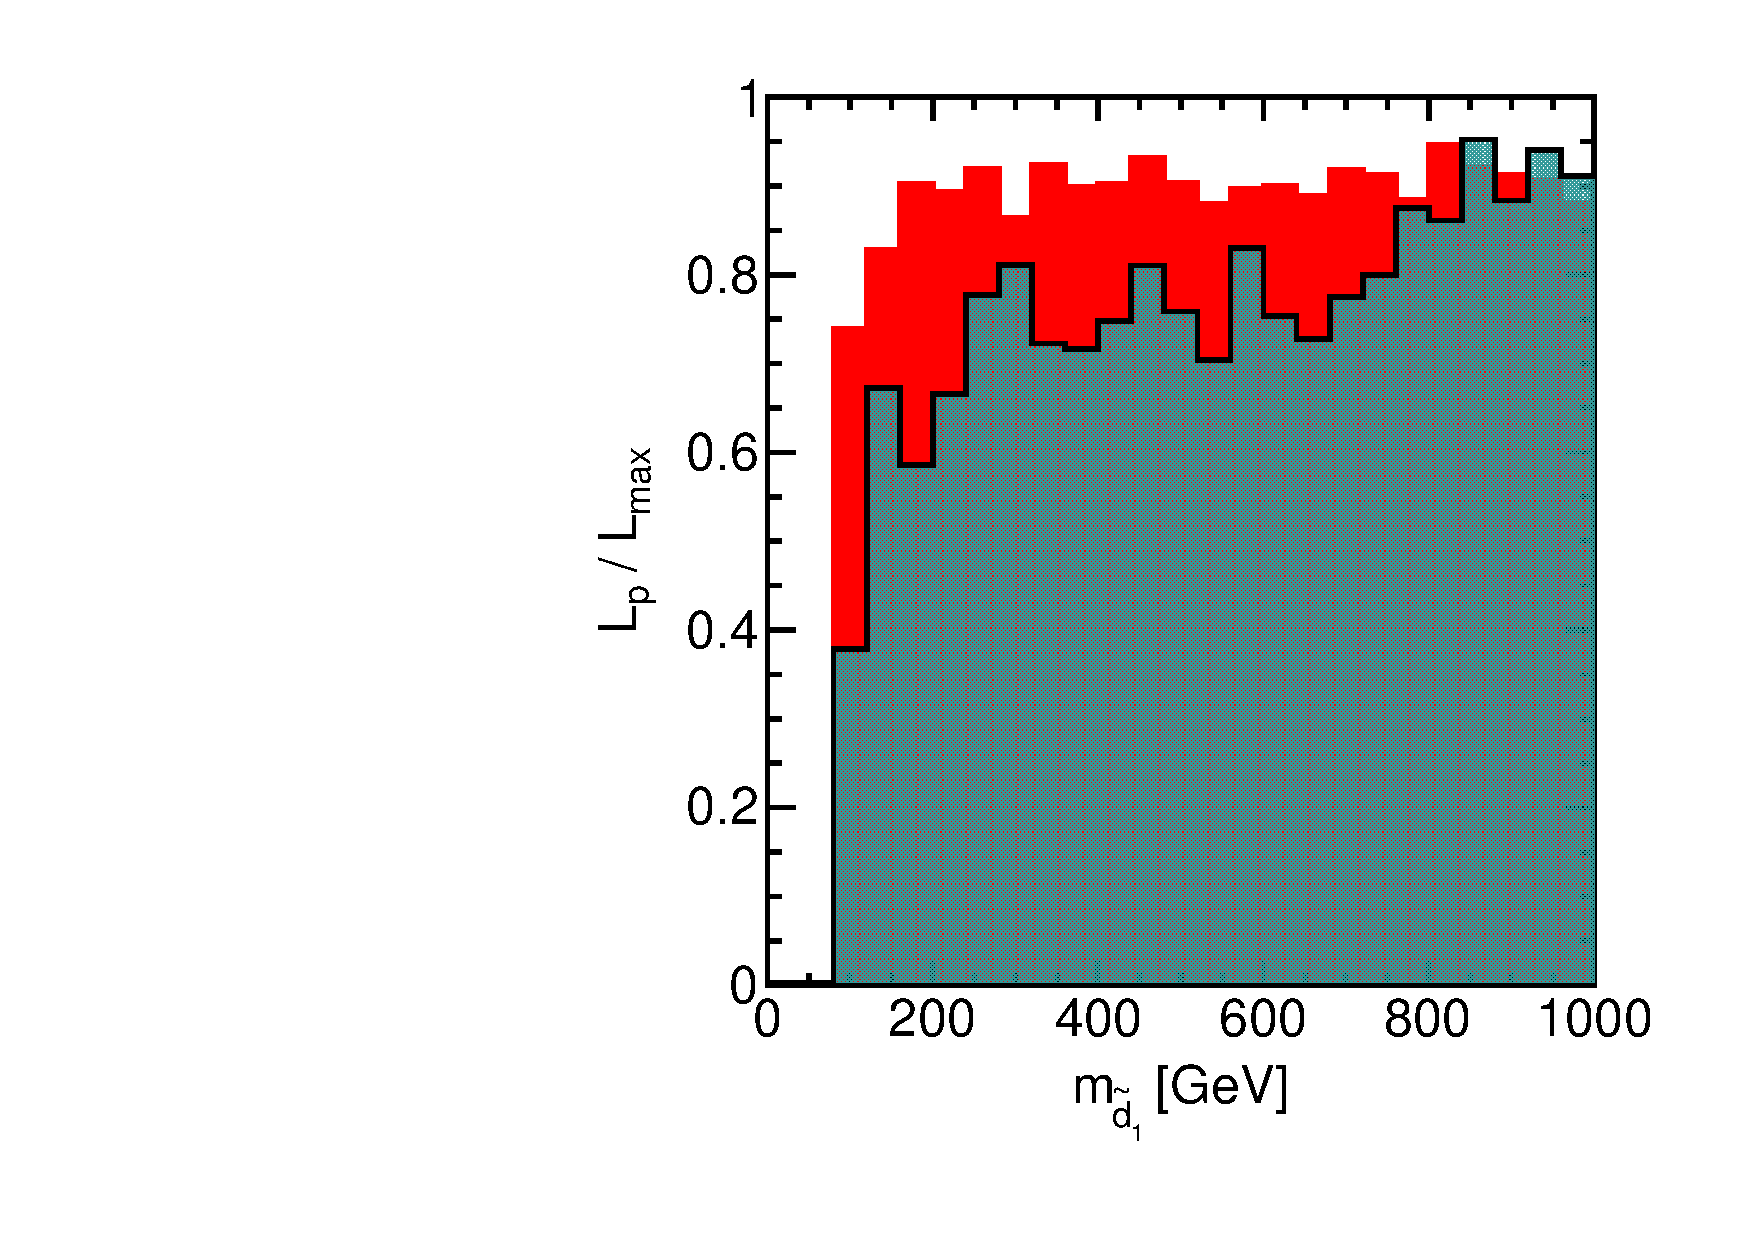
\includegraphics[height=5.5cm]{figs/fig_m_d_1.pdf}
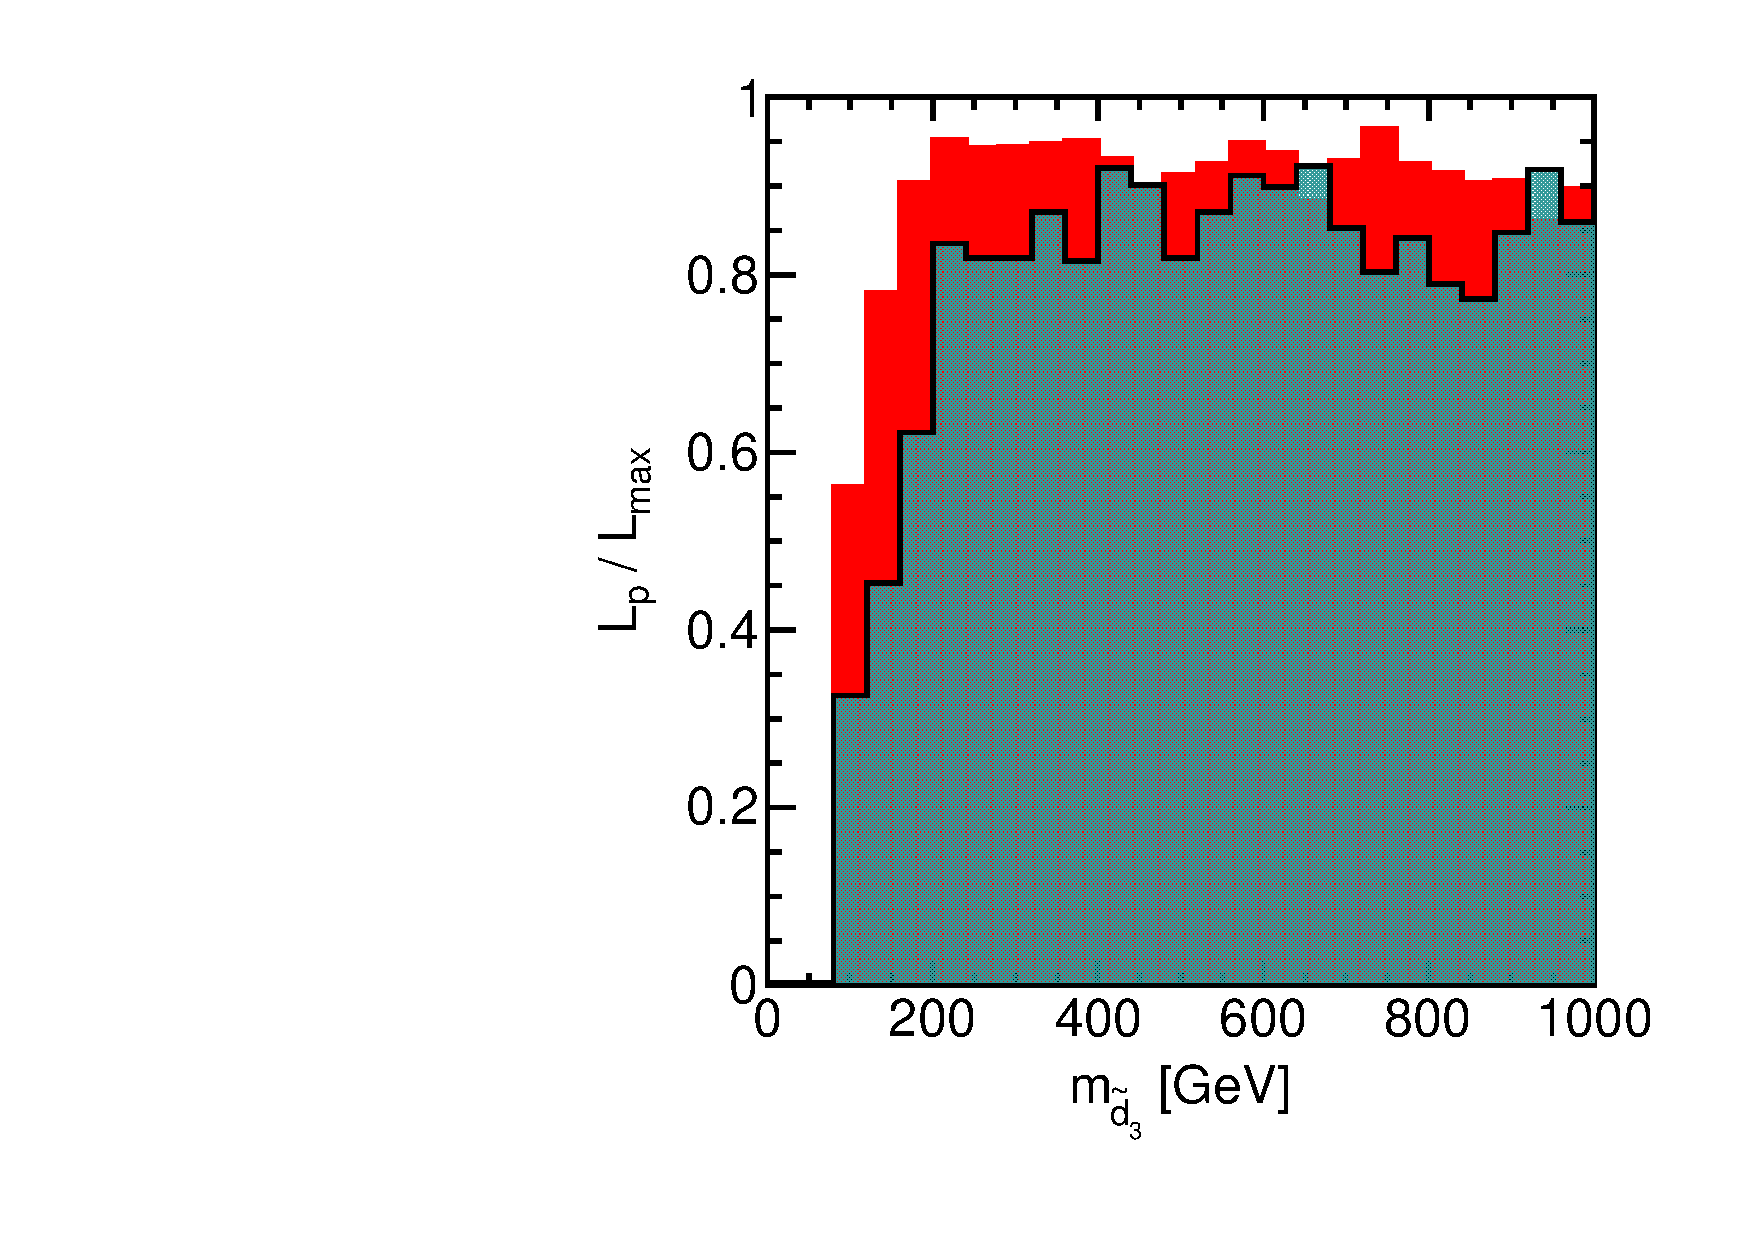
\includegraphics[height=5.5cm]{figs/fig_m_d_3.pdf}
\caption{Ratios of profile likelihood $L_p$ to maximum likelihood $L_{max}$ shown for the squark mass parameters at SUSY scale.  The colored and shaded histograms show the distributions before and after the inclusion of the CMS results.}
\label{fig:LRwcms_msq}
\end{center}
\end{figure}


\begin{figure}[htbp]
\begin{center}
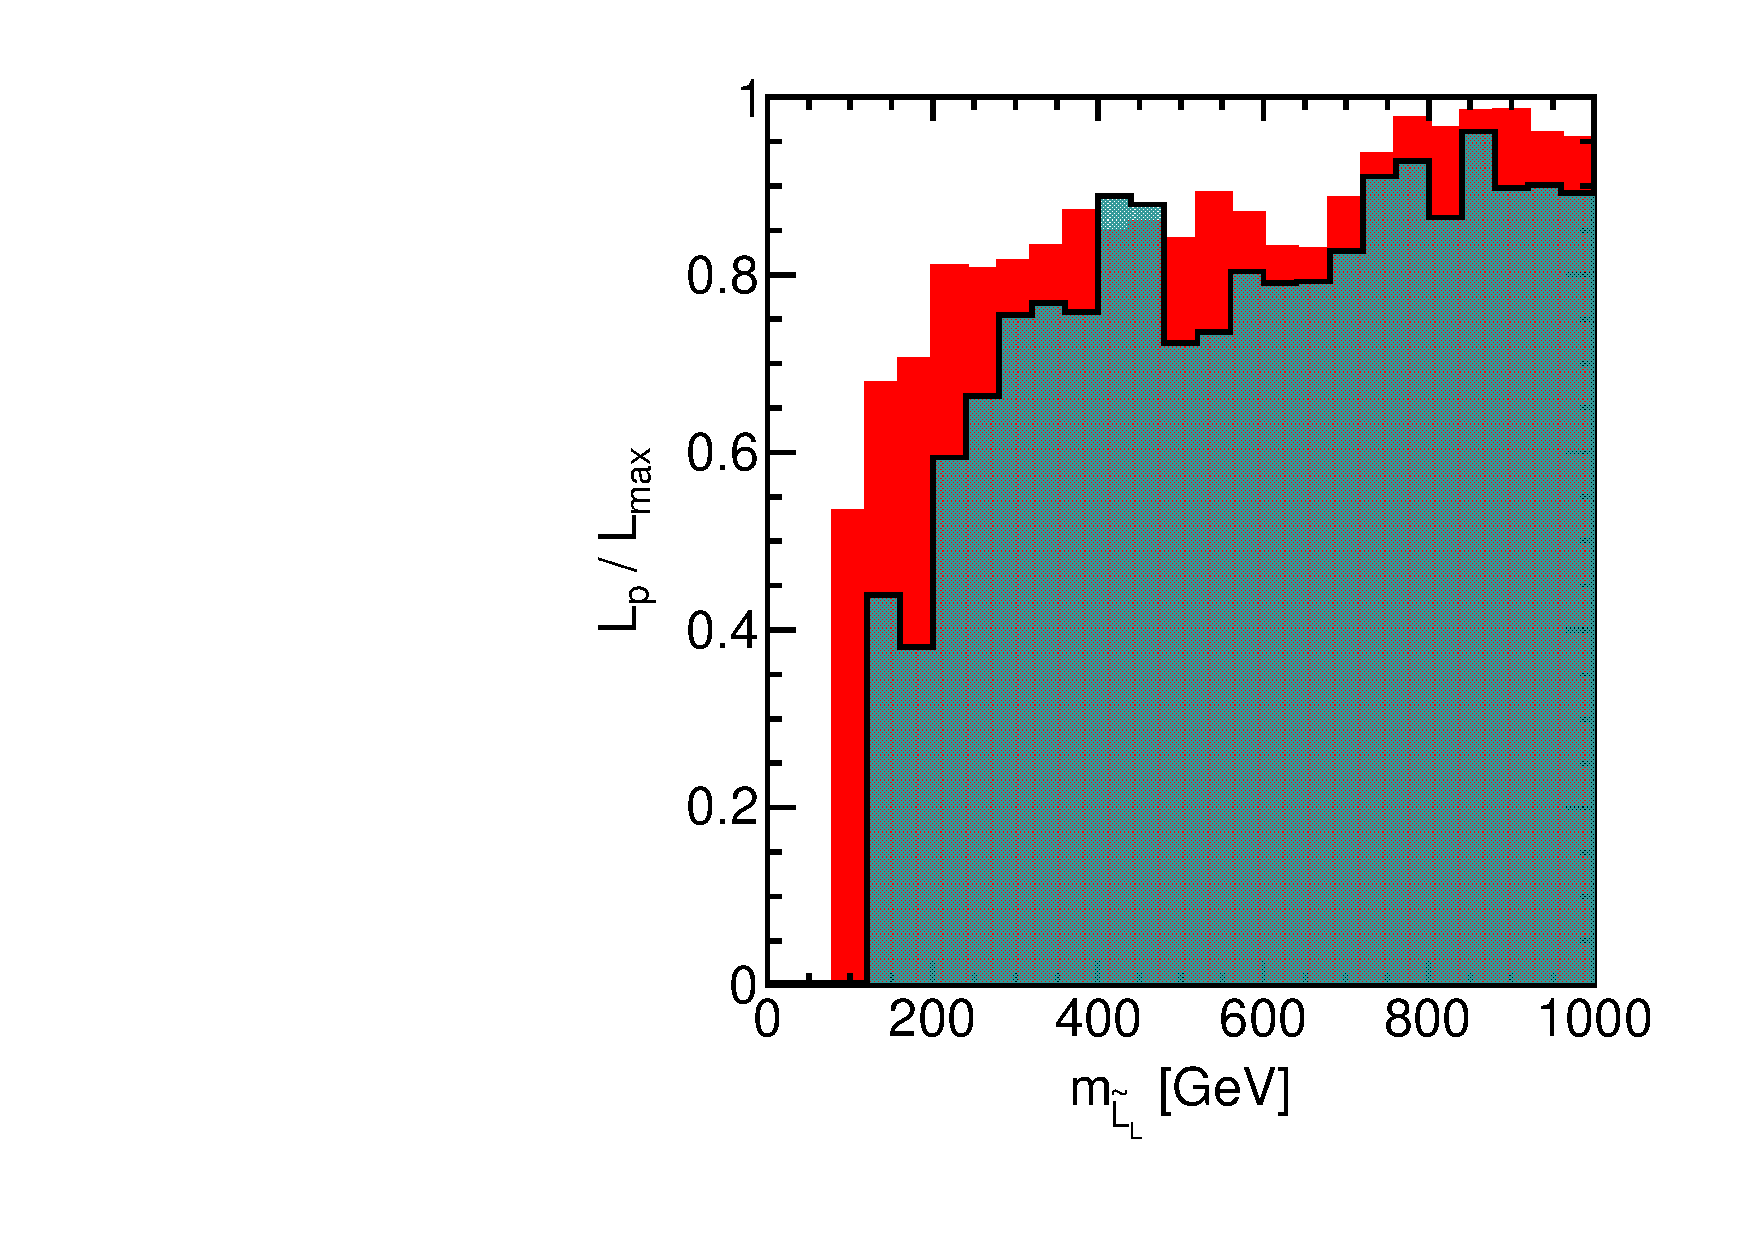
\includegraphics[height=5.5cm]{figs/fig_m_L_L.pdf} 
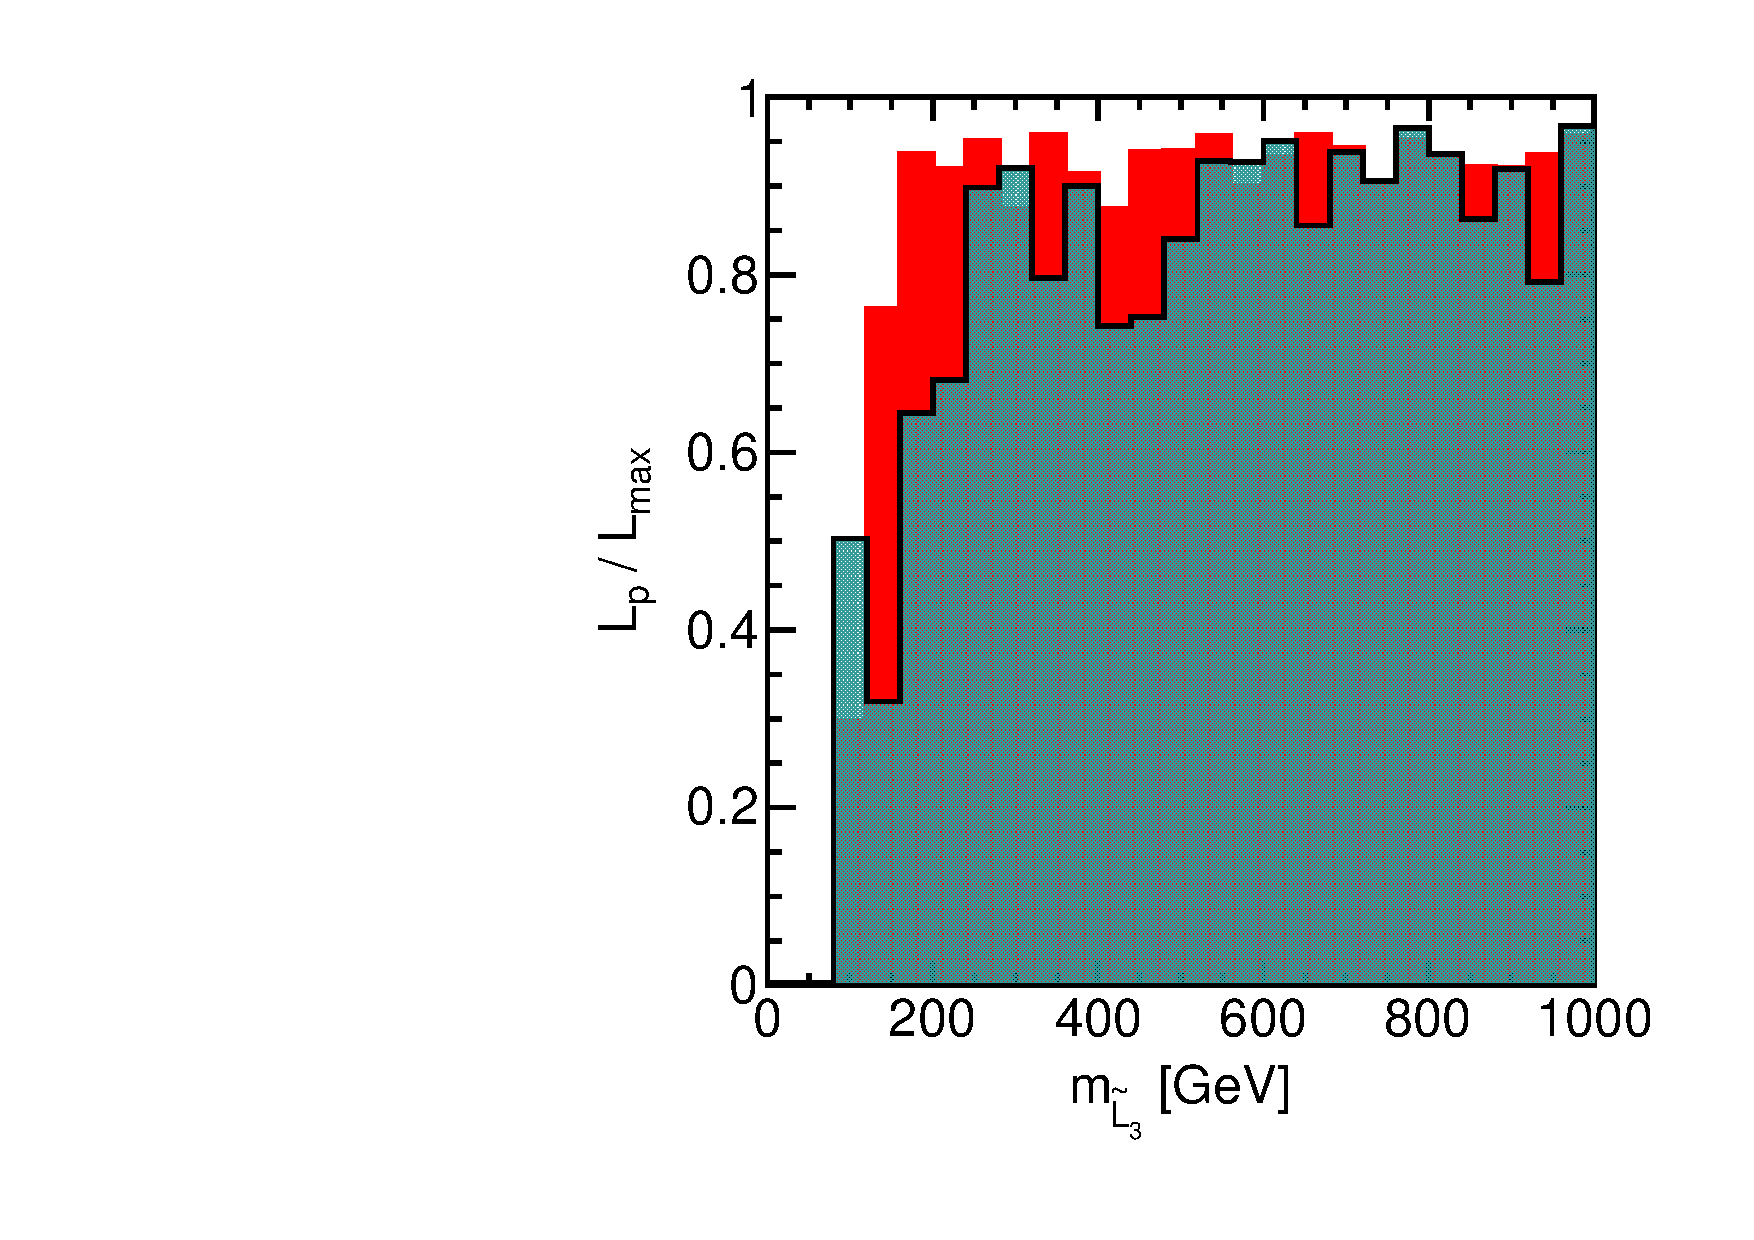
\includegraphics[height=5.5cm]{figs/fig_m_L_3.pdf} \\
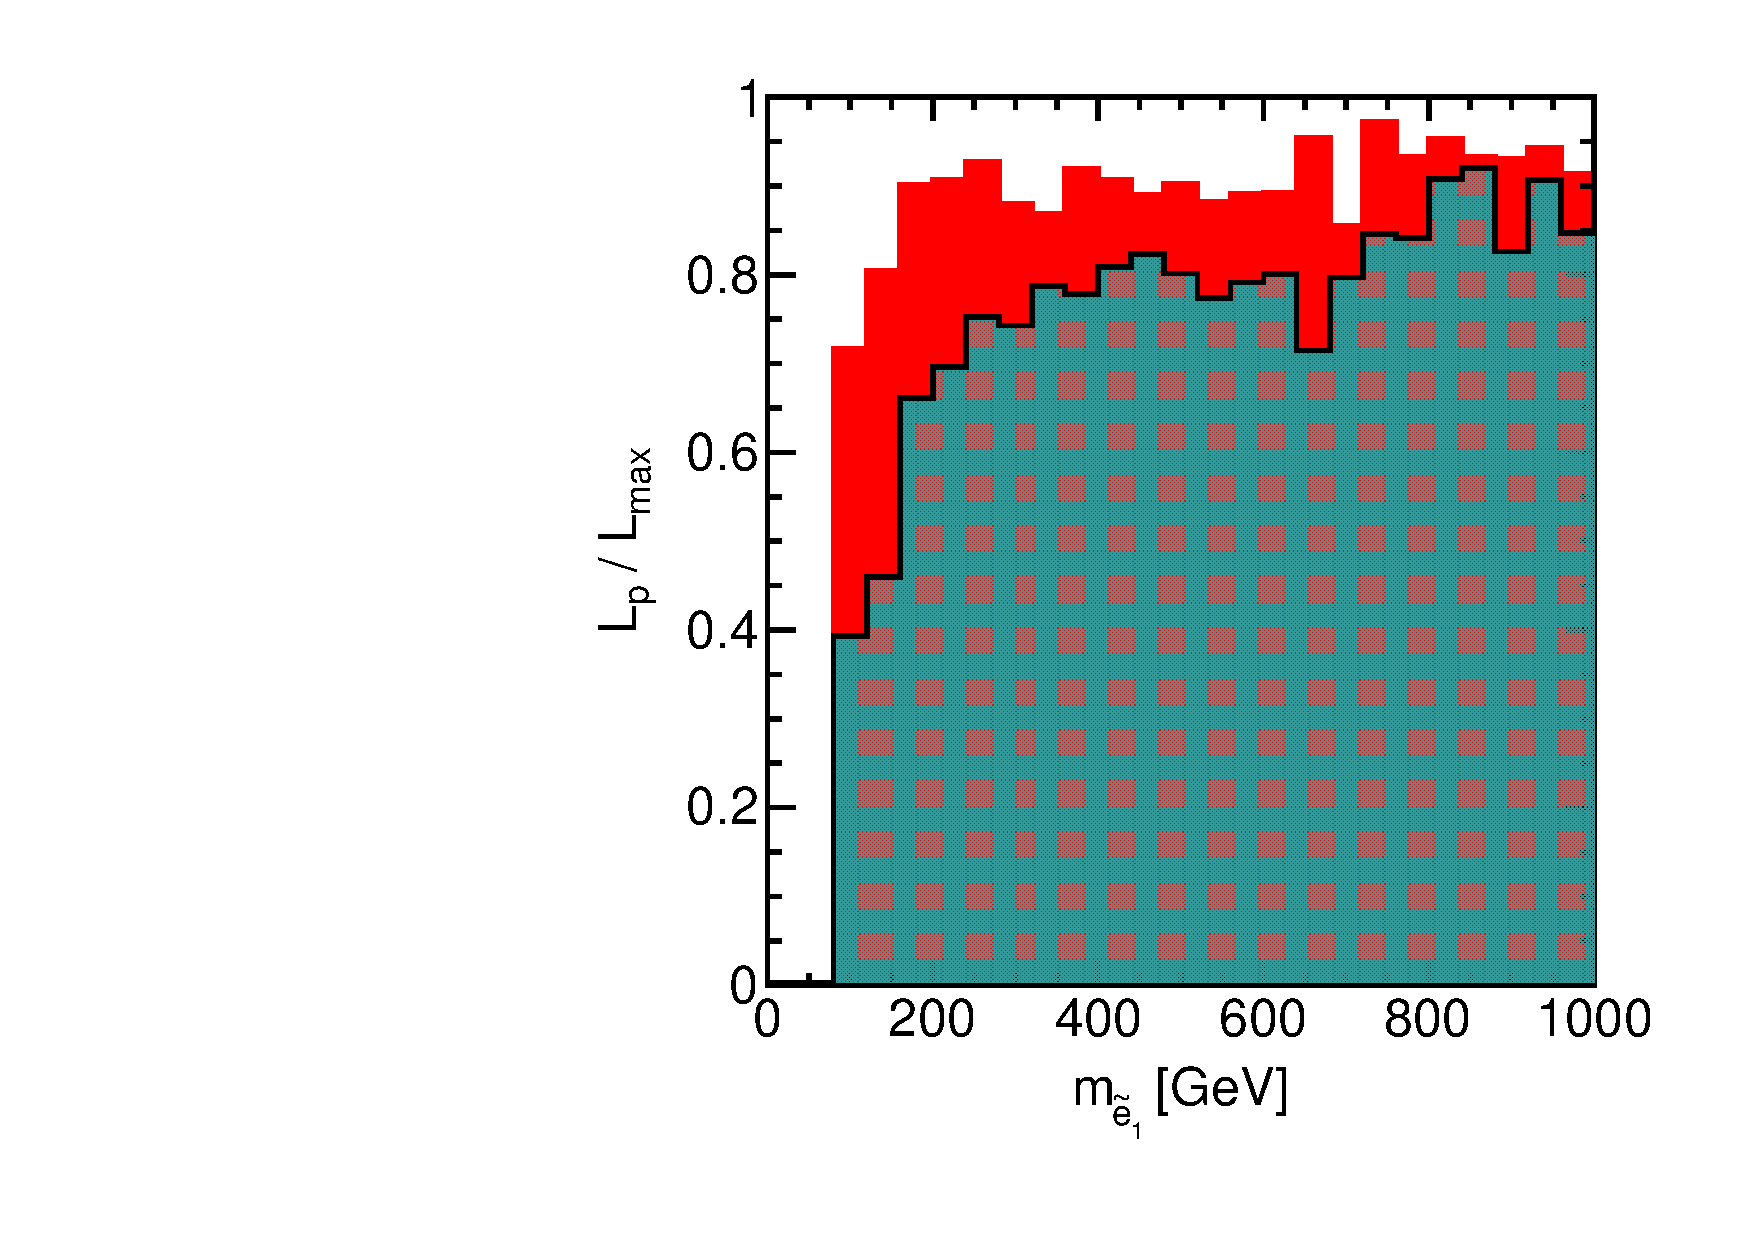
\includegraphics[height=5.5cm]{figs/fig_m_e_1.pdf}
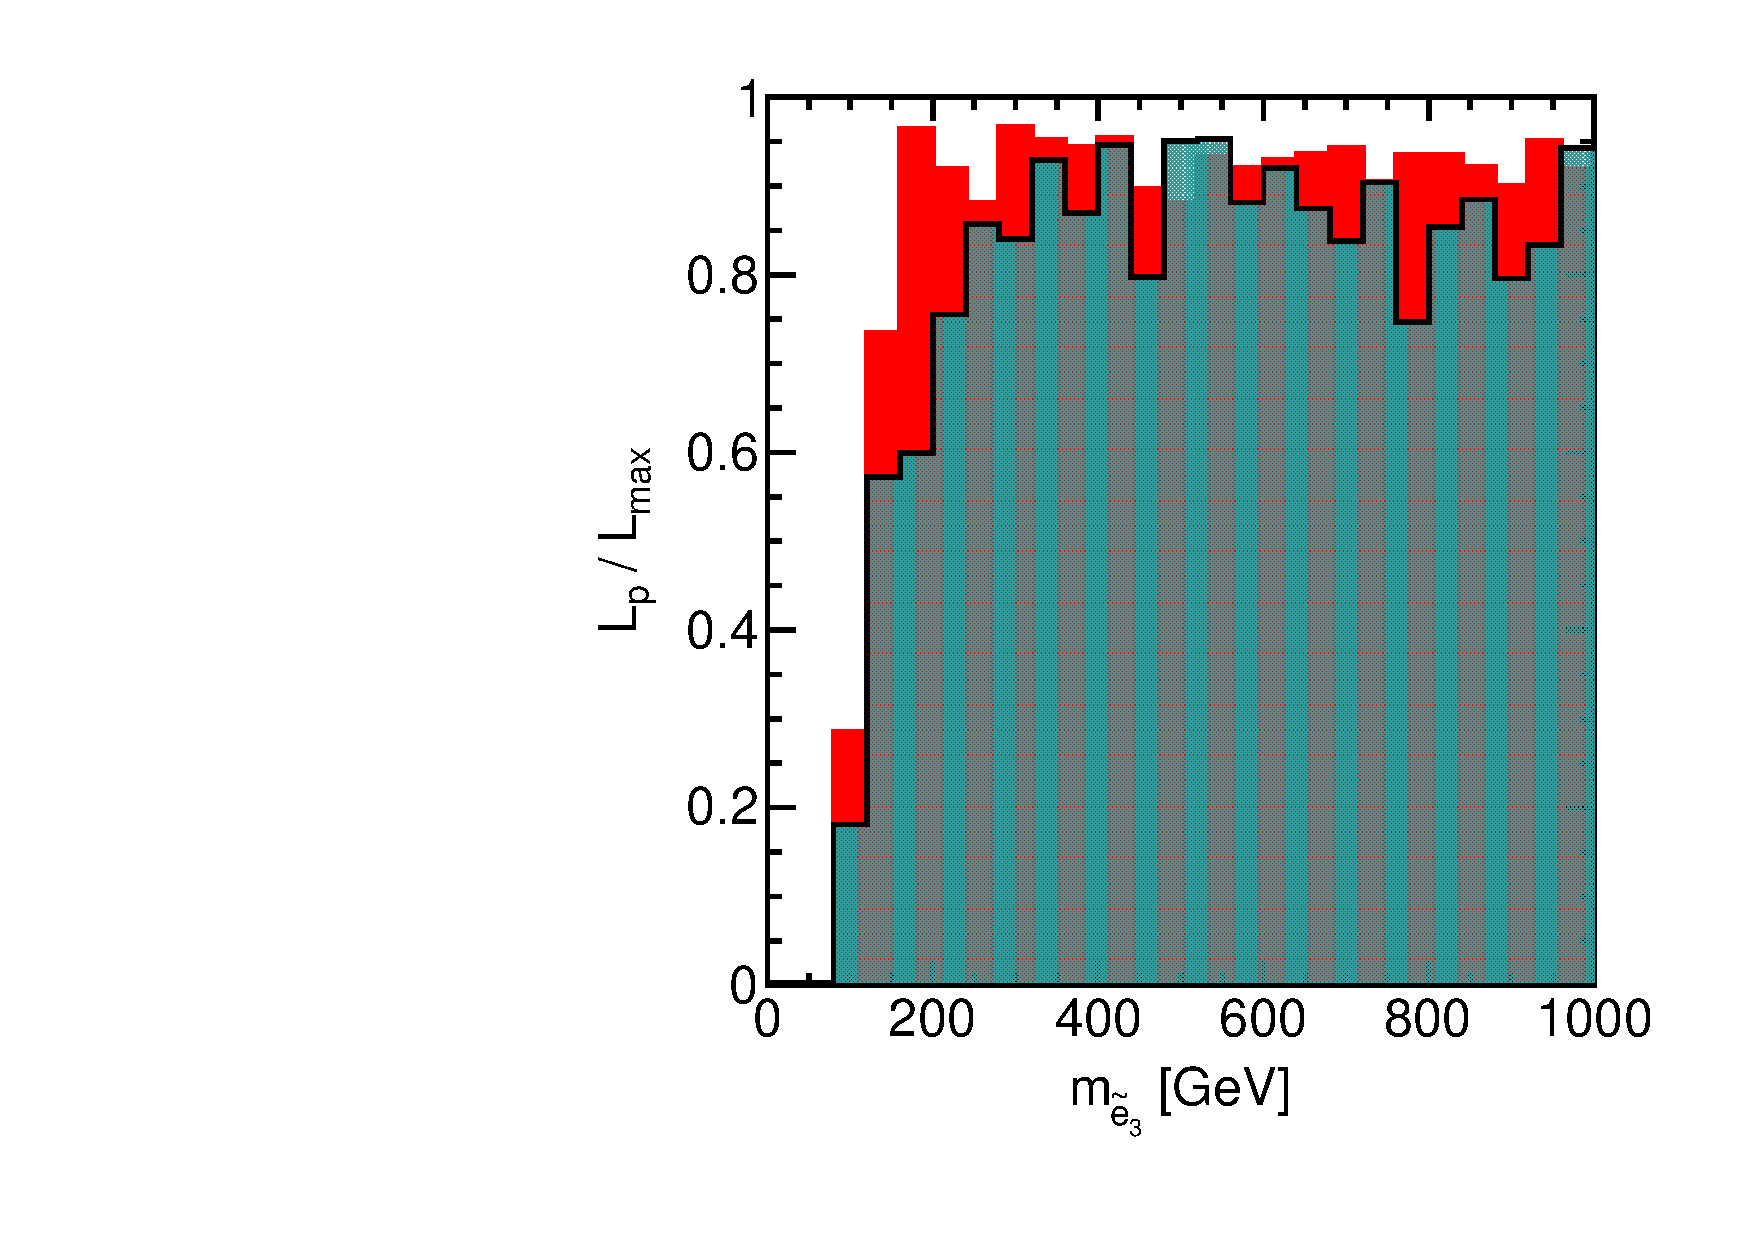
\includegraphics[height=5.5cm]{figs/fig_m_e_3.pdf}
\caption{Ratios of profile likelihood $L_p$ to maximum likelihood $L_{max}$ shown for the slepton mass parameters at SUSY scale.  The colored and shaded histograms show the distributions before and after the inclusion of the CMS results.}
\label{fig:LRwcms_msl}
\end{center}
\end{figure}


\begin{figure}[htbp]
\begin{center}
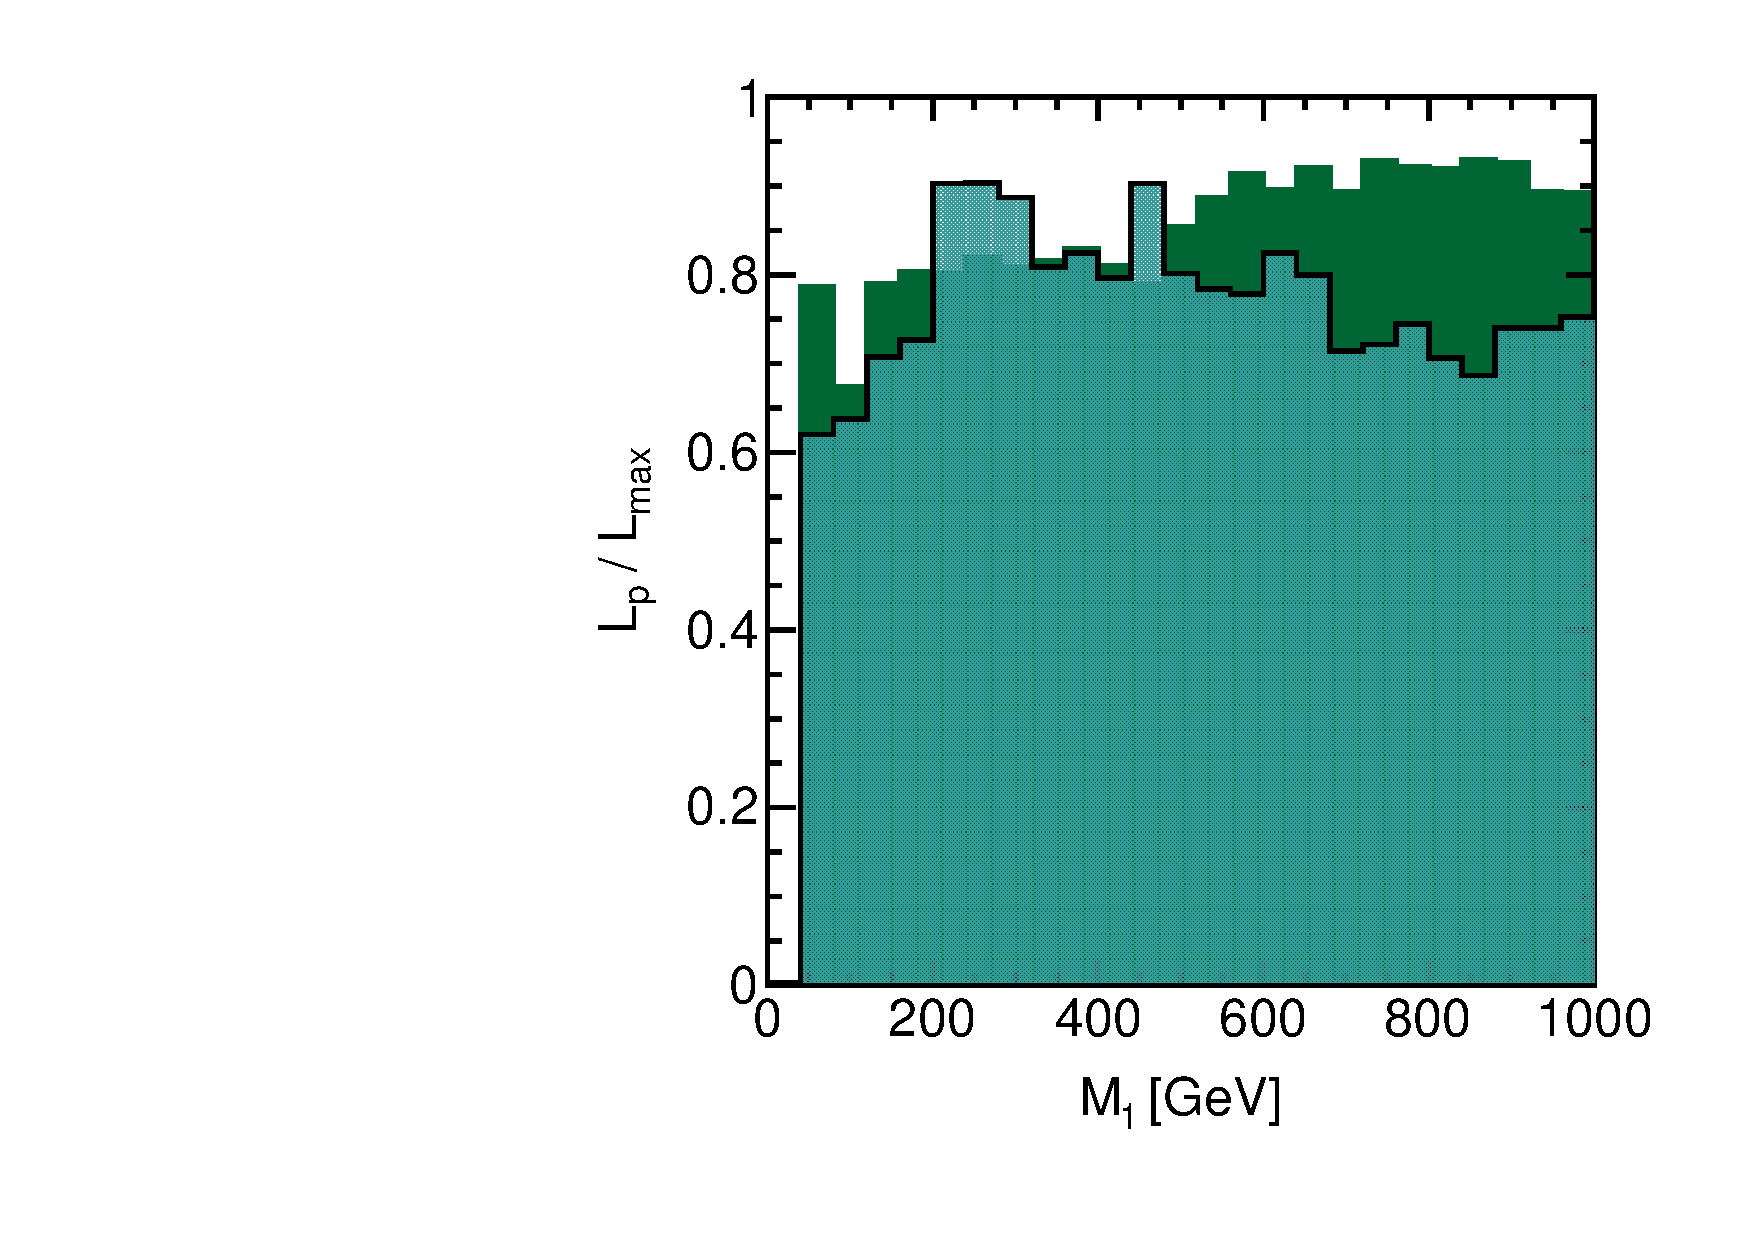
\includegraphics[height=5.5cm]{figs/fig_M_1.pdf} 
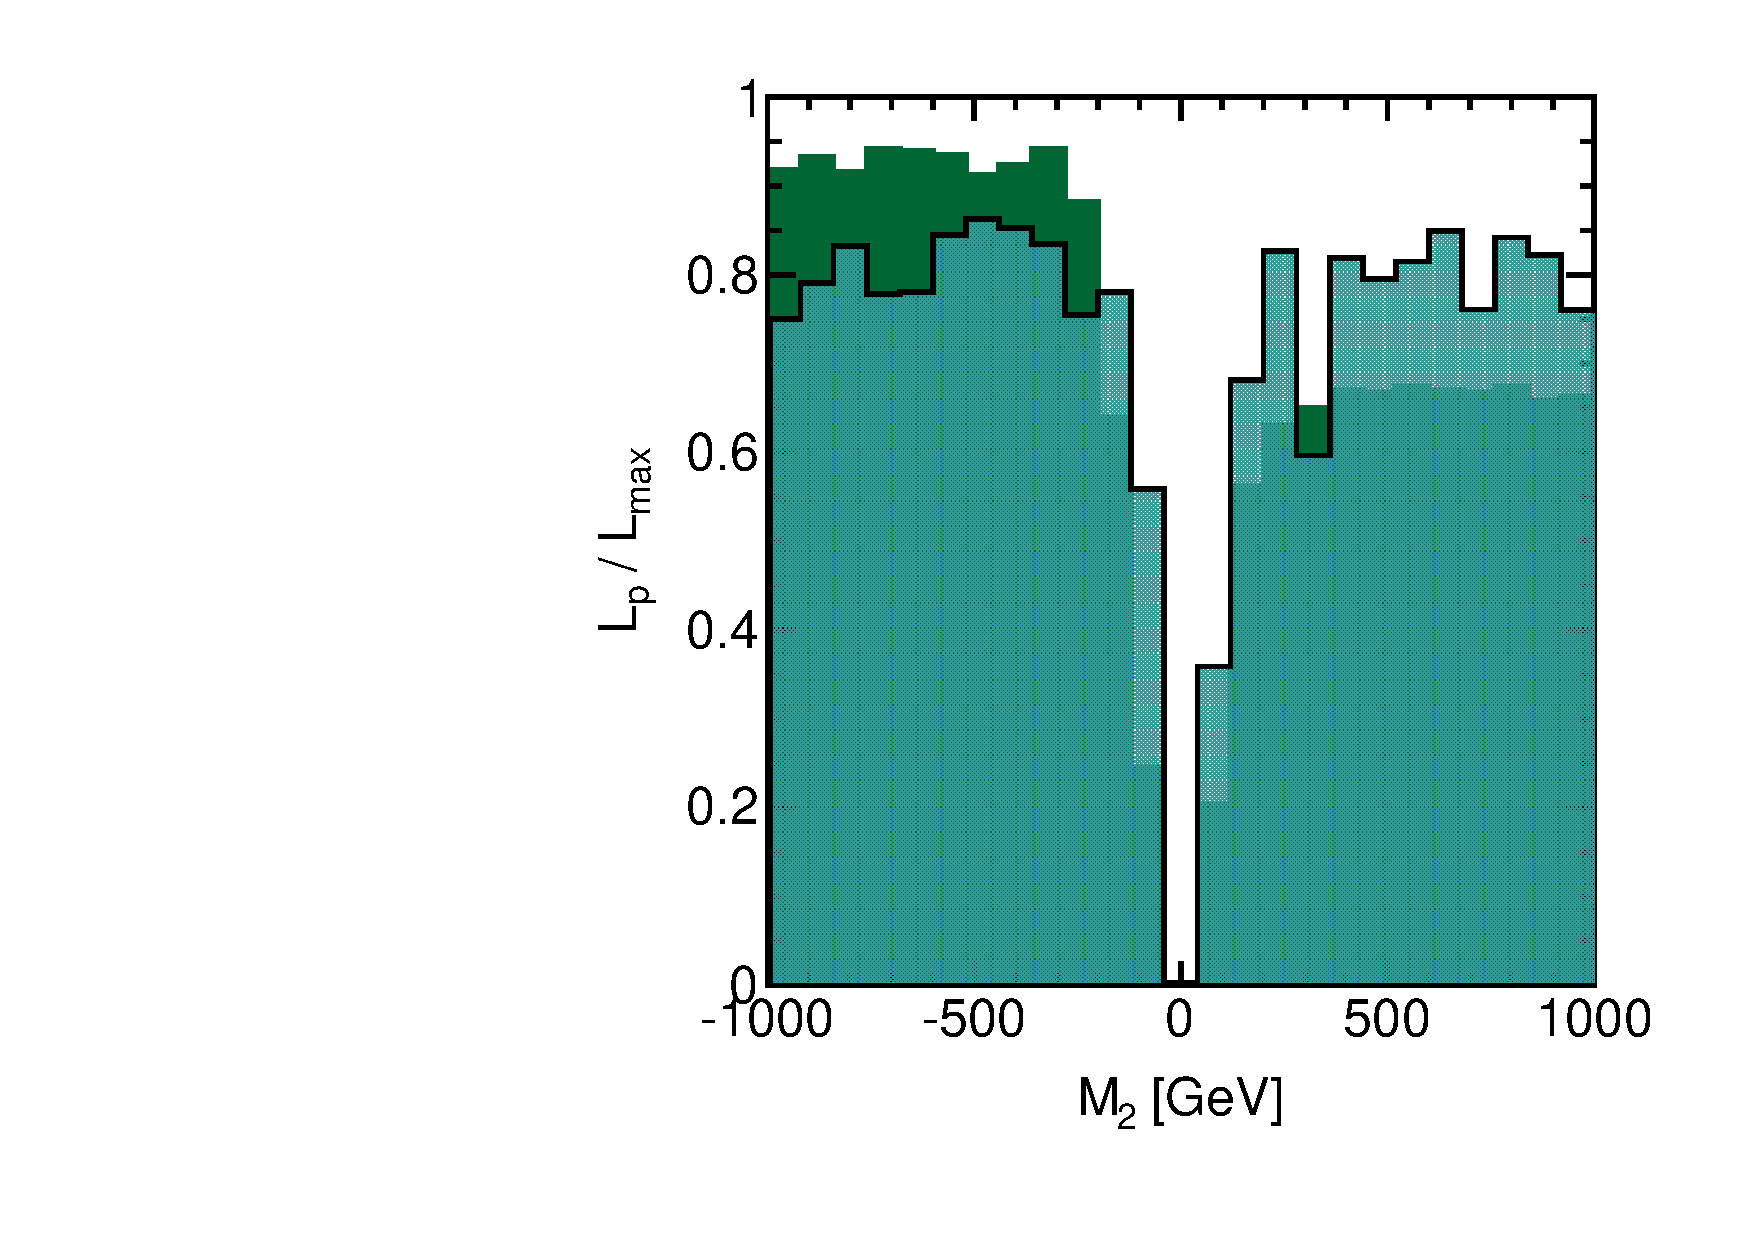
\includegraphics[height=5.5cm]{figs/fig_M_2.pdf} \\
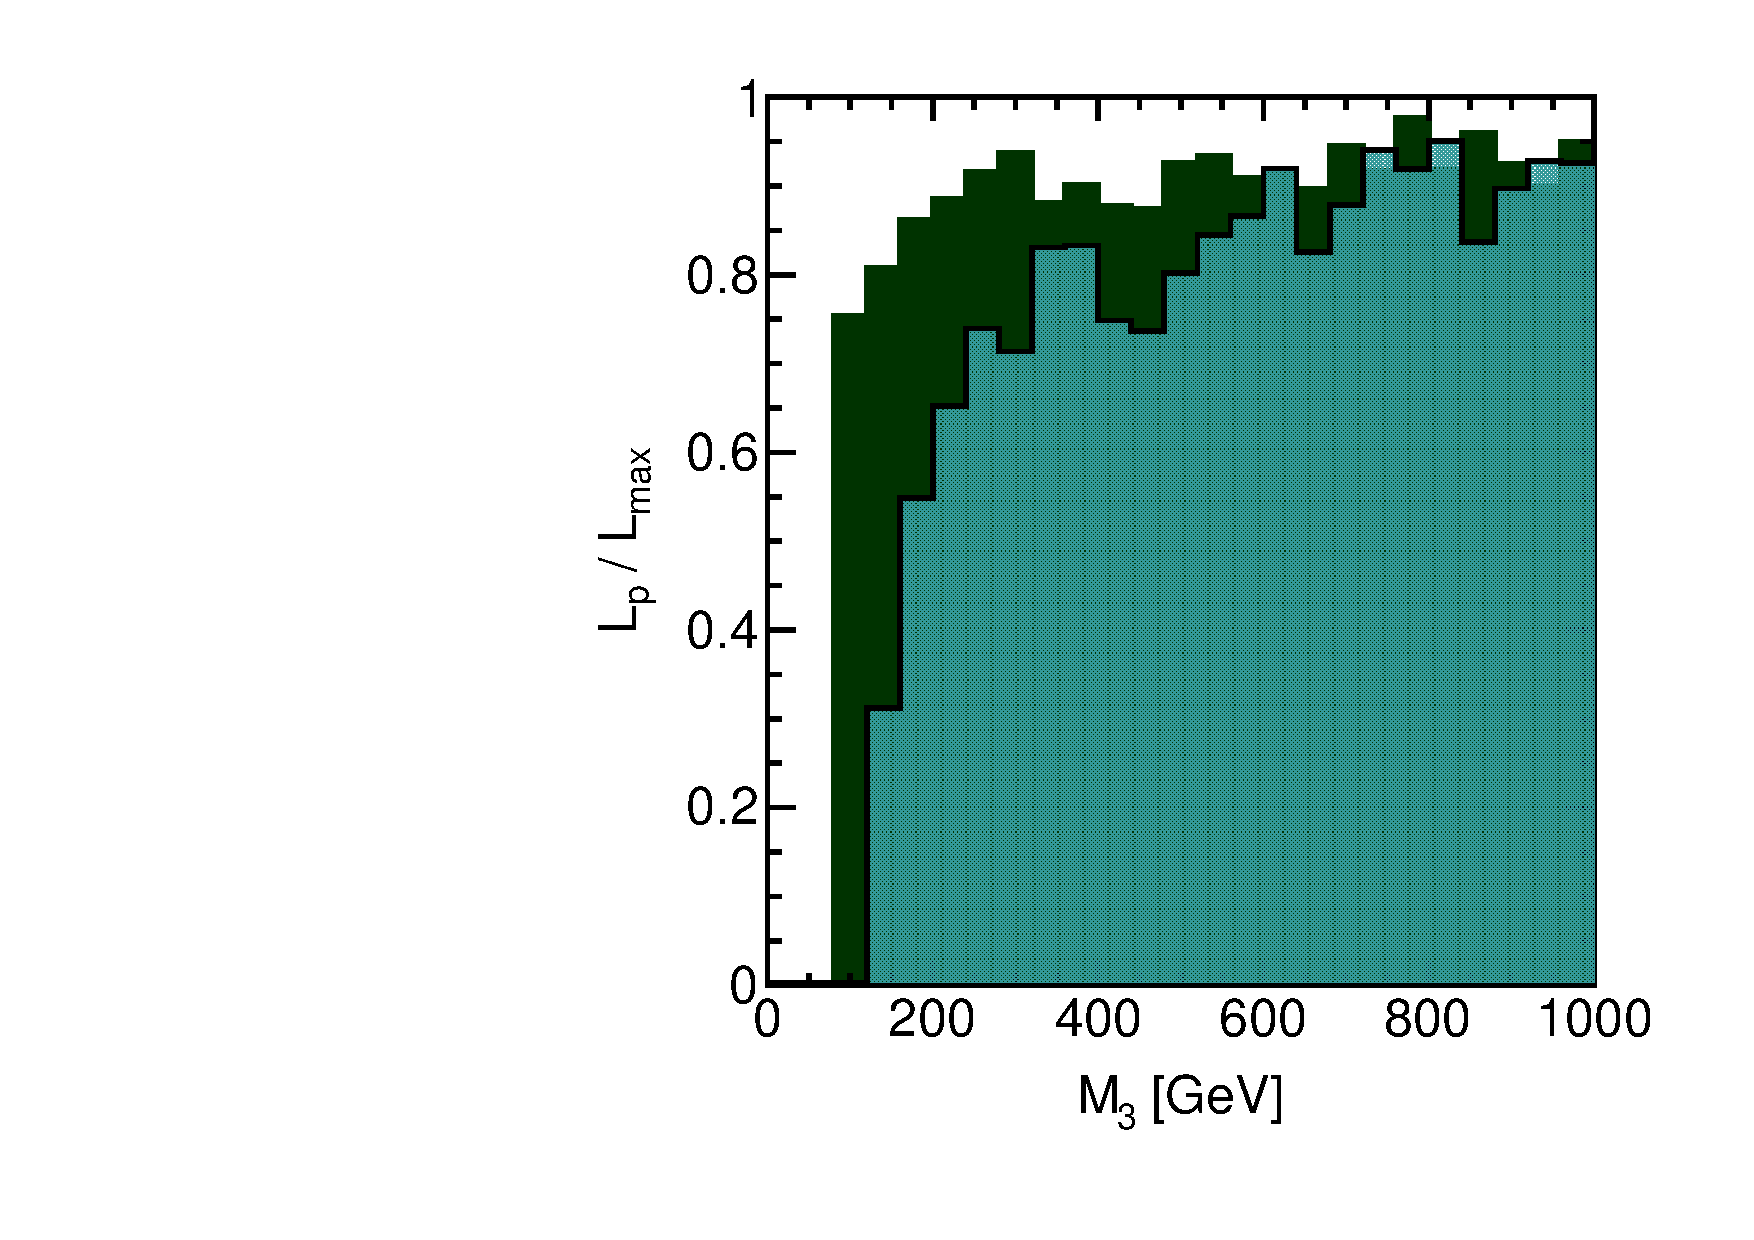
\includegraphics[height=5.5cm]{figs/fig_M_3.pdf}
\caption{Ratios of profile likelihood $L_p$ to maximum likelihood $L_{max}$ shown for gaugino mass parameters at  SUSY scale.  The colored and shaded histograms show the distributions before and after the inclusion of the CMS results.}
\label{fig:LRwcms_M}
\end{center}
\end{figure}


\begin{figure}[htbp]
\begin{center}
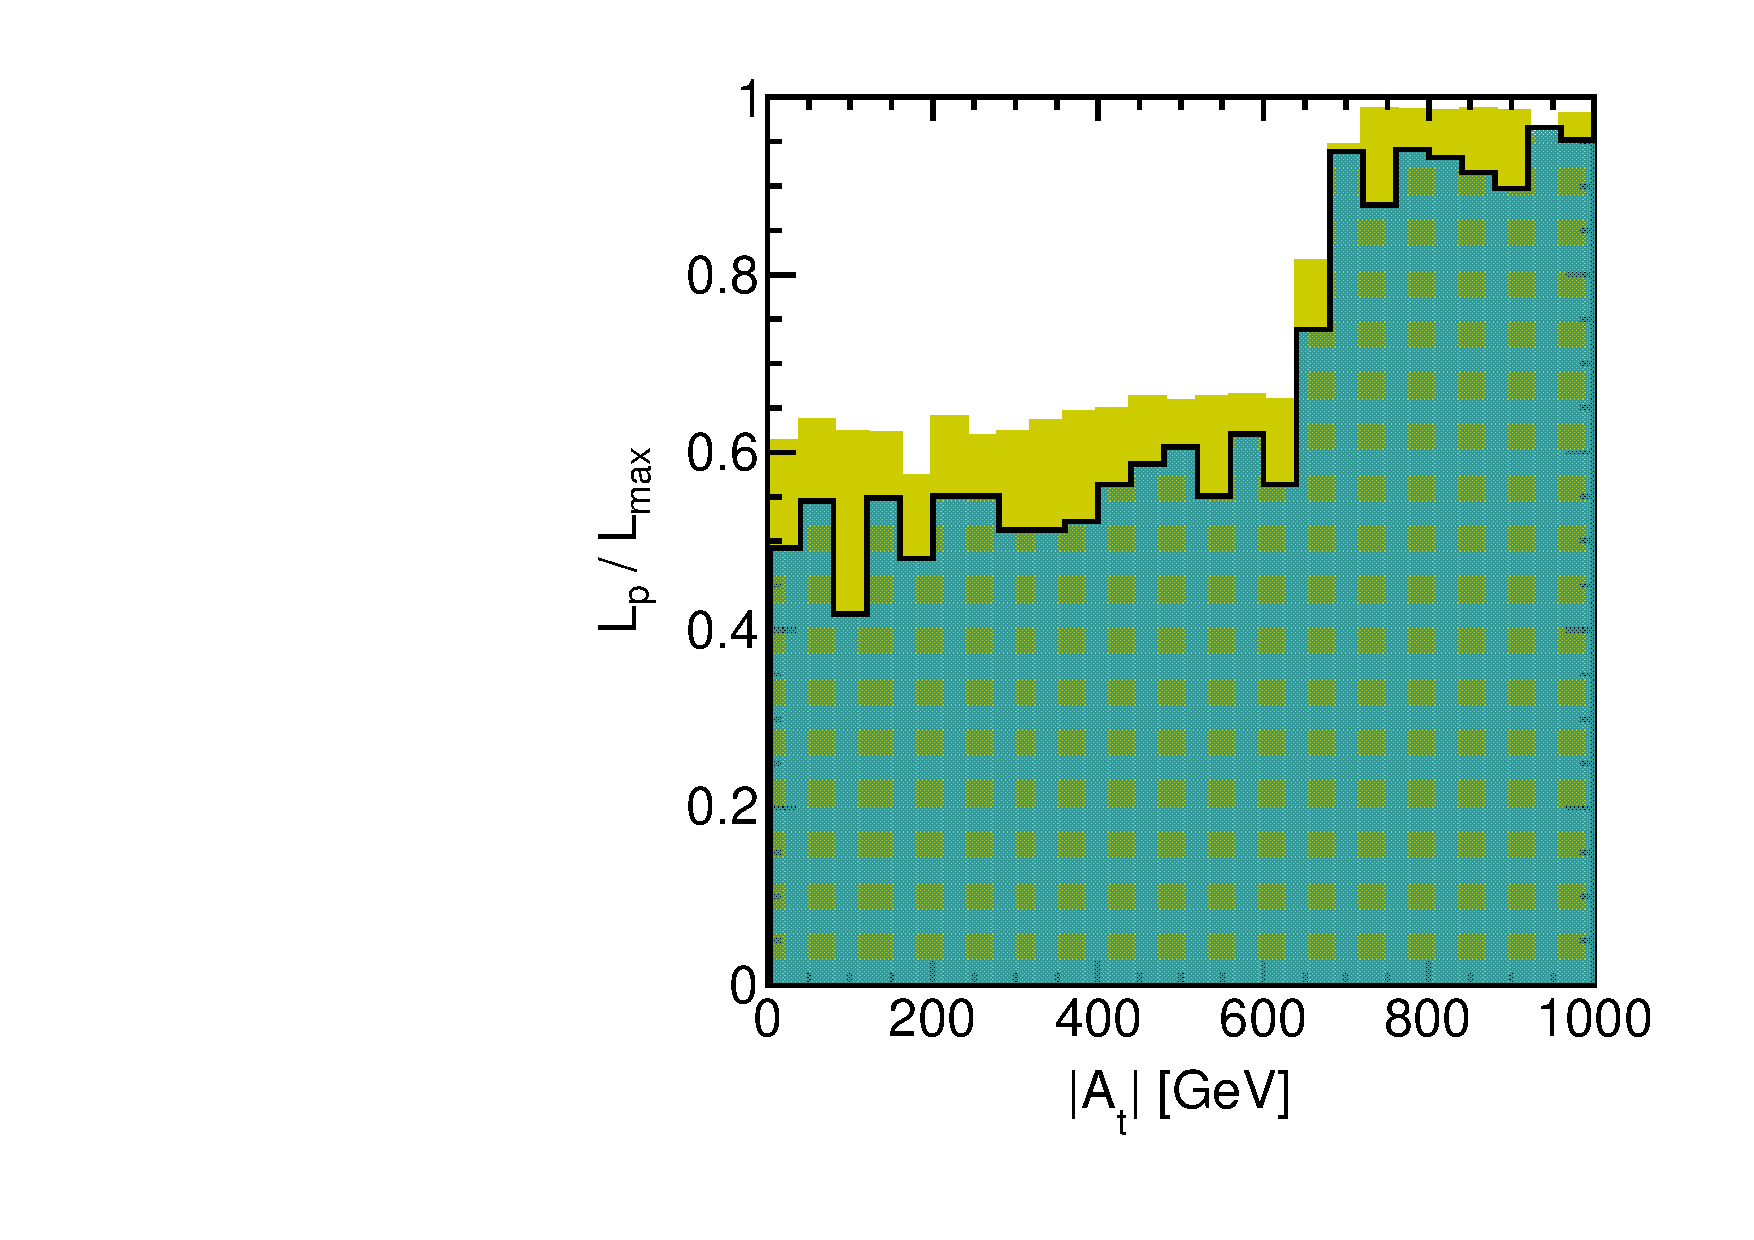
\includegraphics[height=5.5cm]{figs/fig_A_t.pdf} 
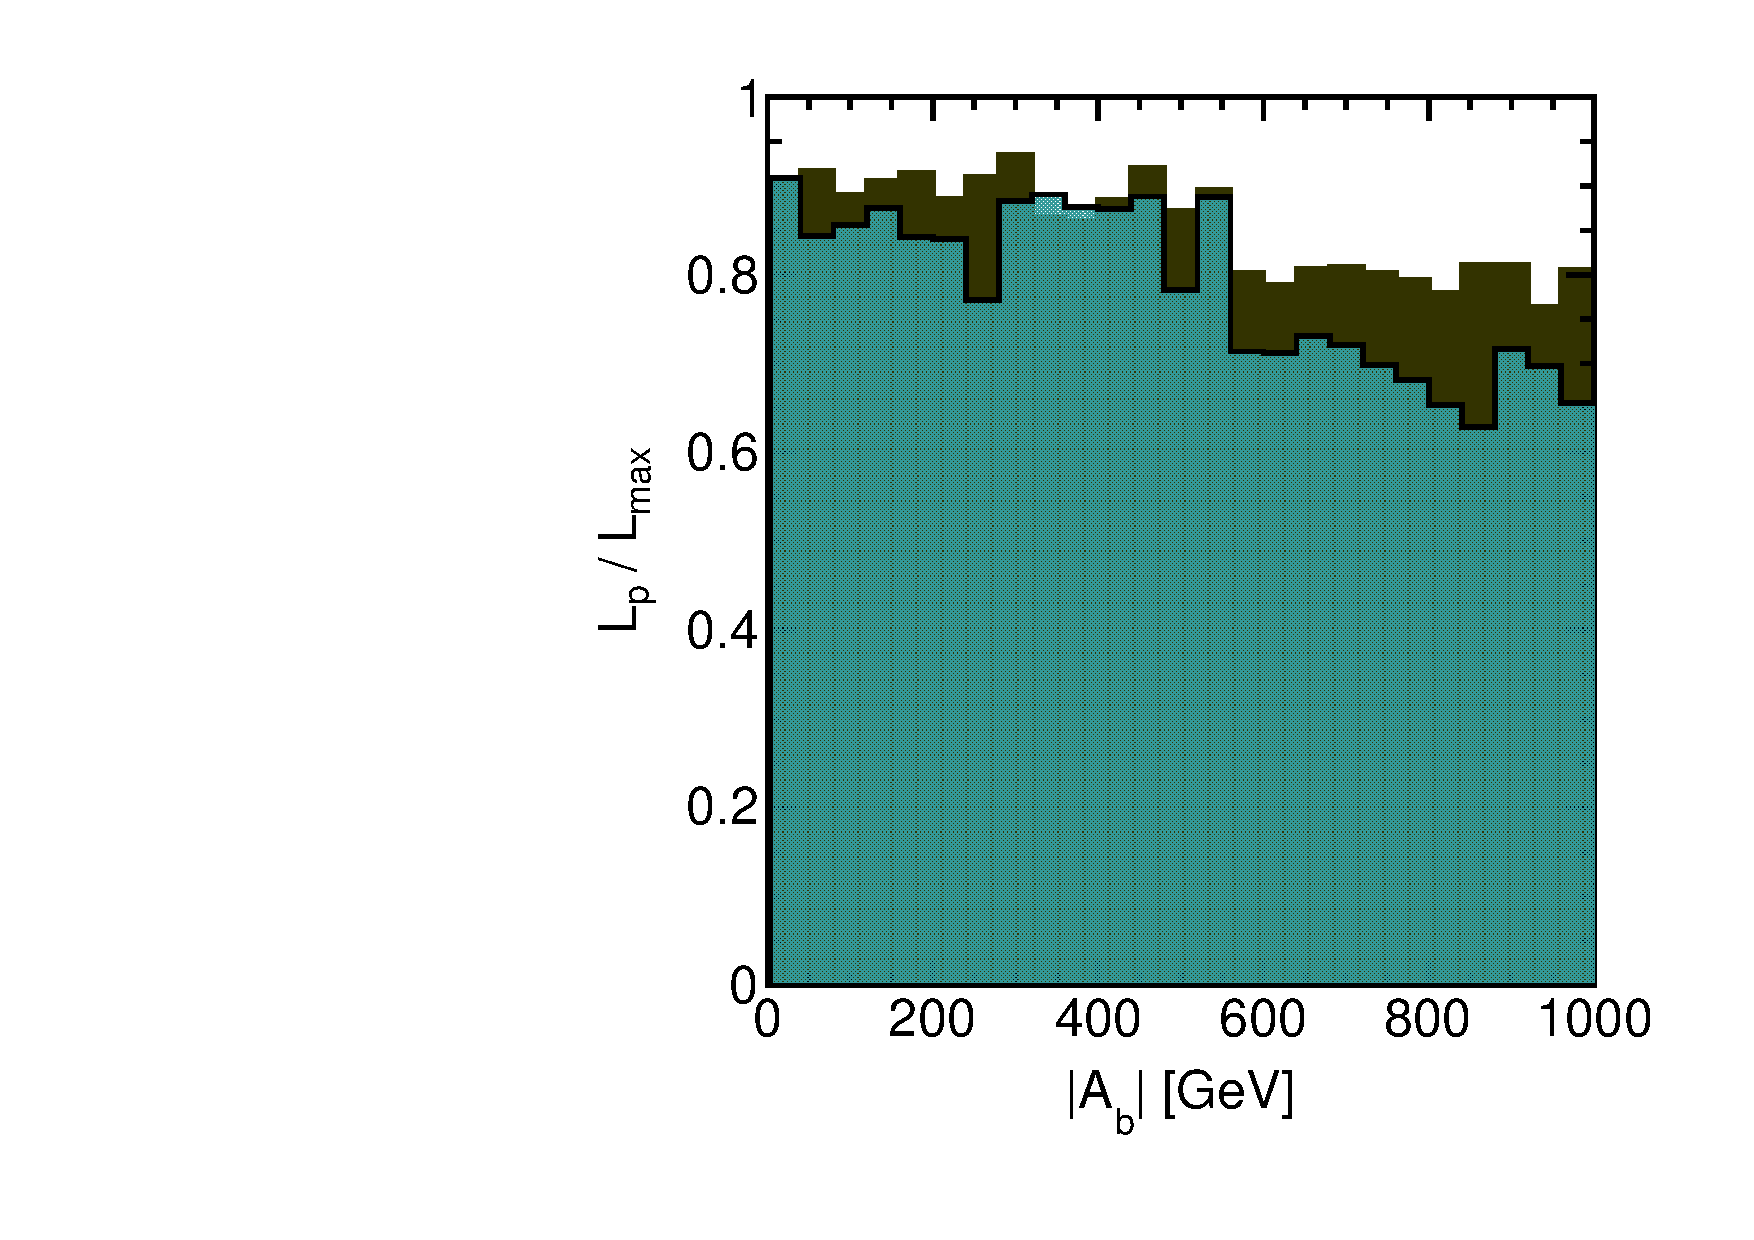
\includegraphics[height=5.5cm]{figs/fig_A_b.pdf} \\
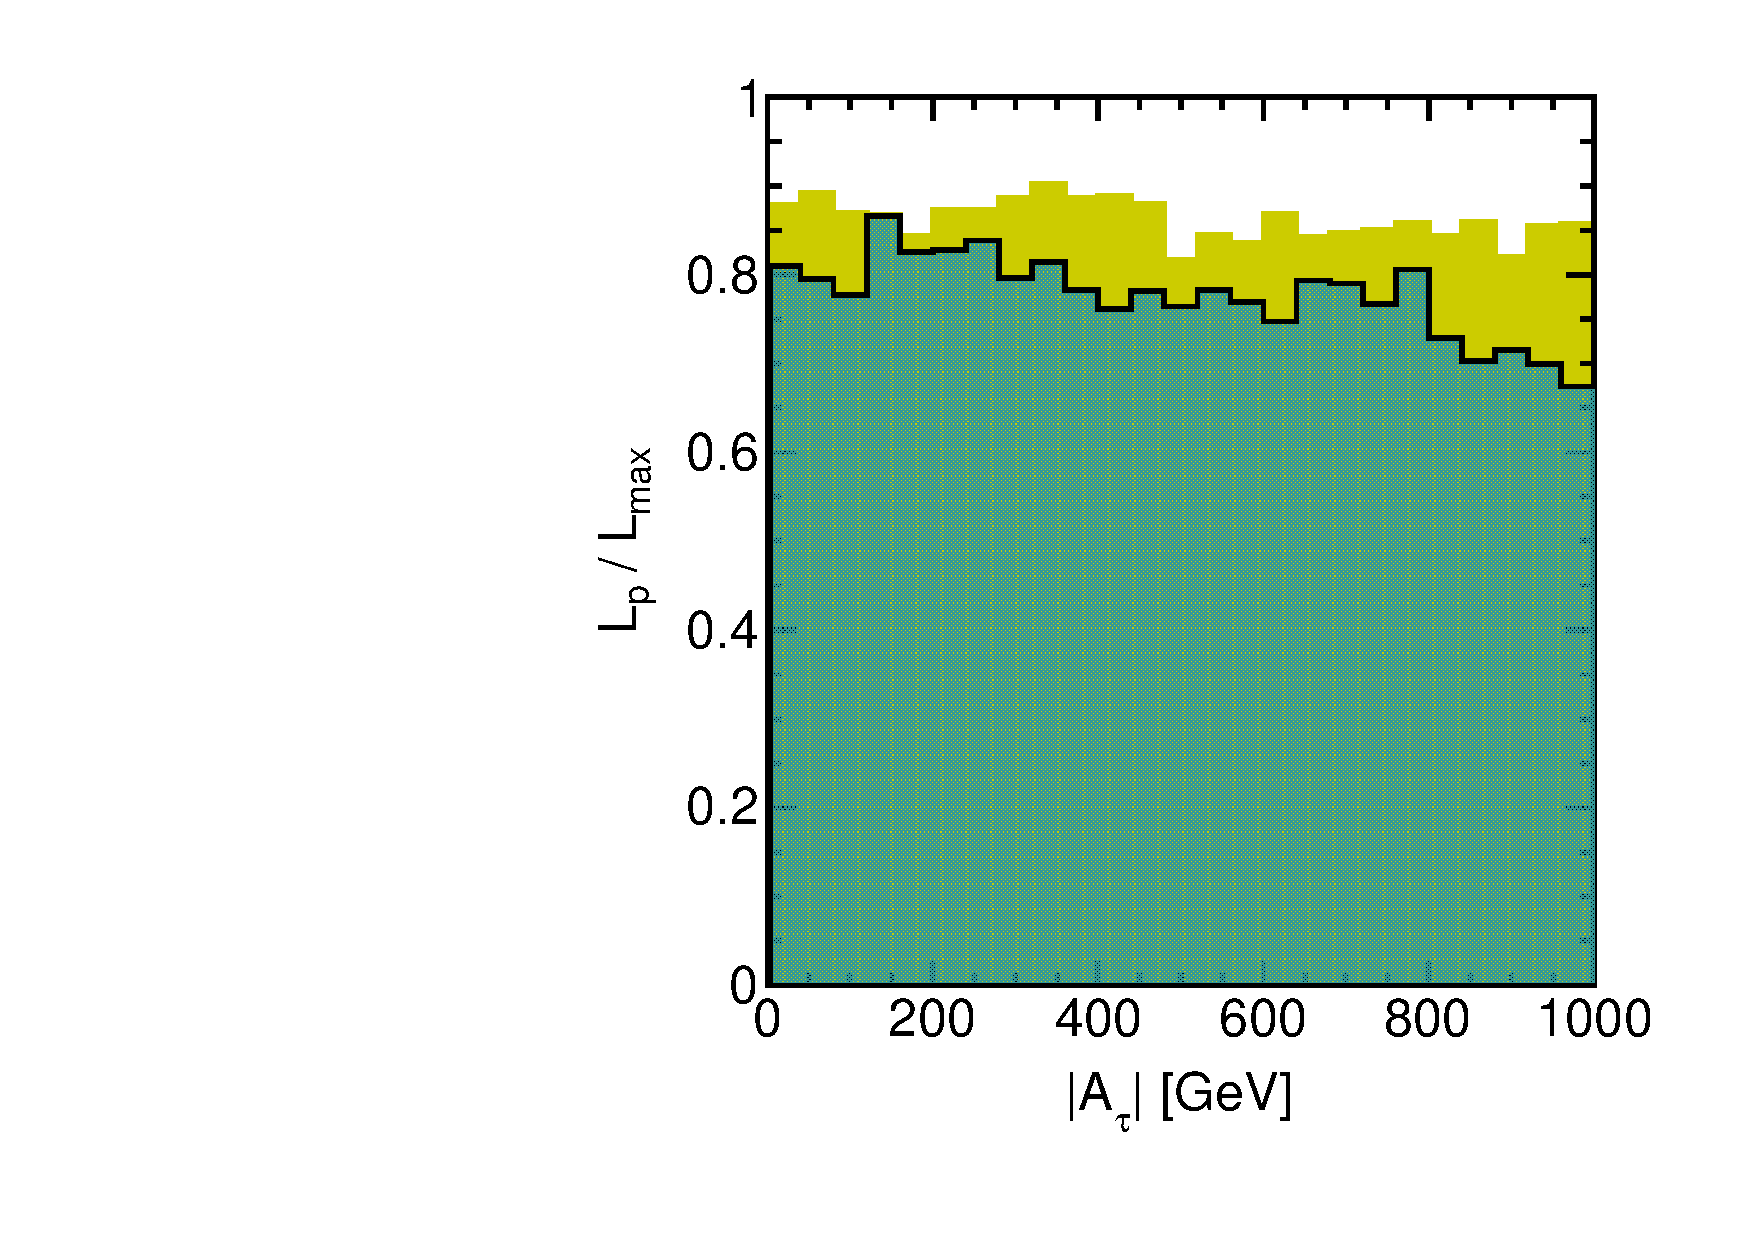
\includegraphics[height=5.5cm]{figs/fig_A_tau.pdf}
\caption{Ratios of profile likelihood $L_p$ to maximum likelihood $L_{max}$ shown for trilinear couplings at SUSY scale.  The colored and shaded histograms show the distributions before and after the inclusion of the CMS results.}
\label{fig:LRwcms_A}
\end{center}
\end{figure}

\begin{figure}[htbp]
\begin{center}
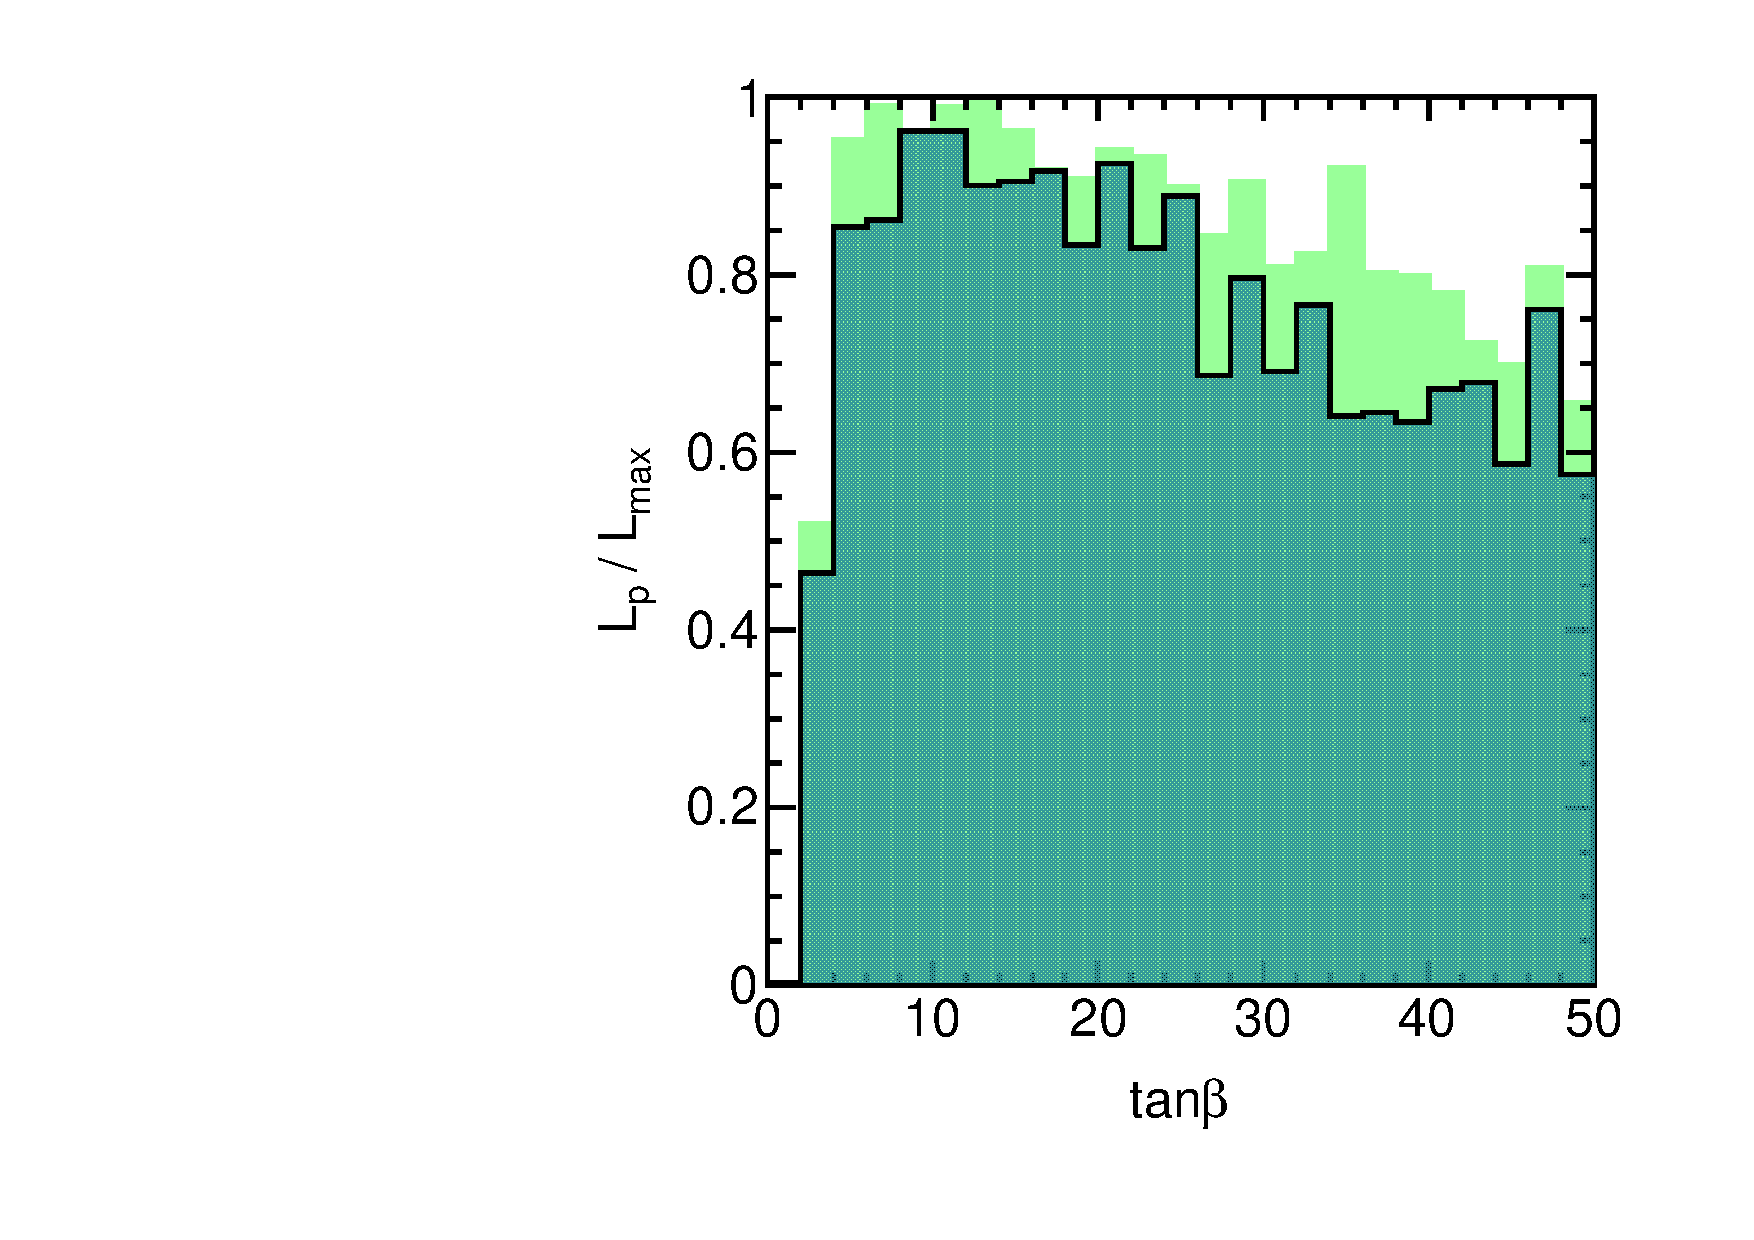
\includegraphics[height=5.5cm]{figs/fig_tanbeta.pdf} 
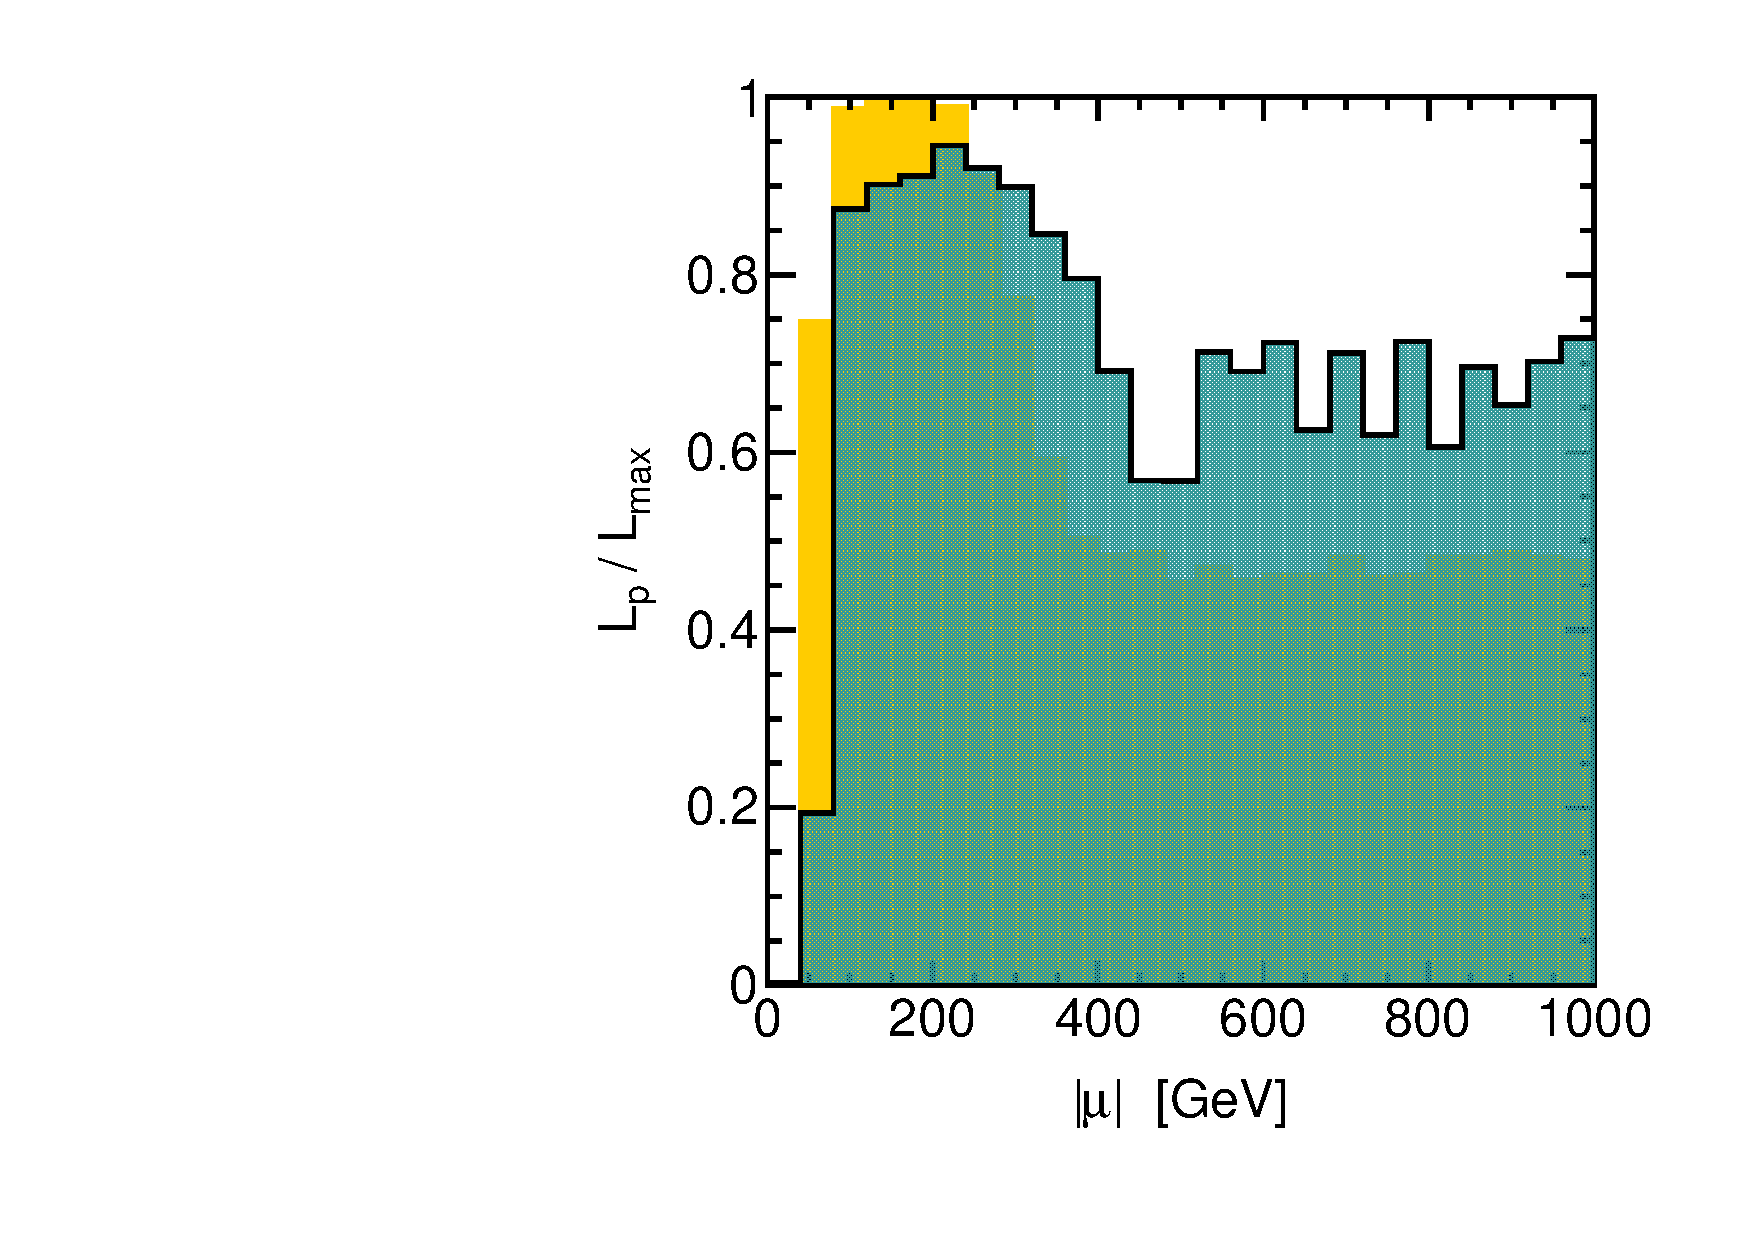
\includegraphics[height=5.5cm]{figs/fig_mu.pdf} 
\caption{Ratios of profile likelihood $L_p$ to maximum likelihood $L_{max}$ shown for $\tan\beta$ and $\mu$ parameter at SUSY scale.  The colored and shaded histograms show the distributions before and after the inclusion of the CMS results.}
\label{fig:LRwcms_tbmu}
\end{center}
\end{figure}



\begin{figure}[htbp]
\begin{center}
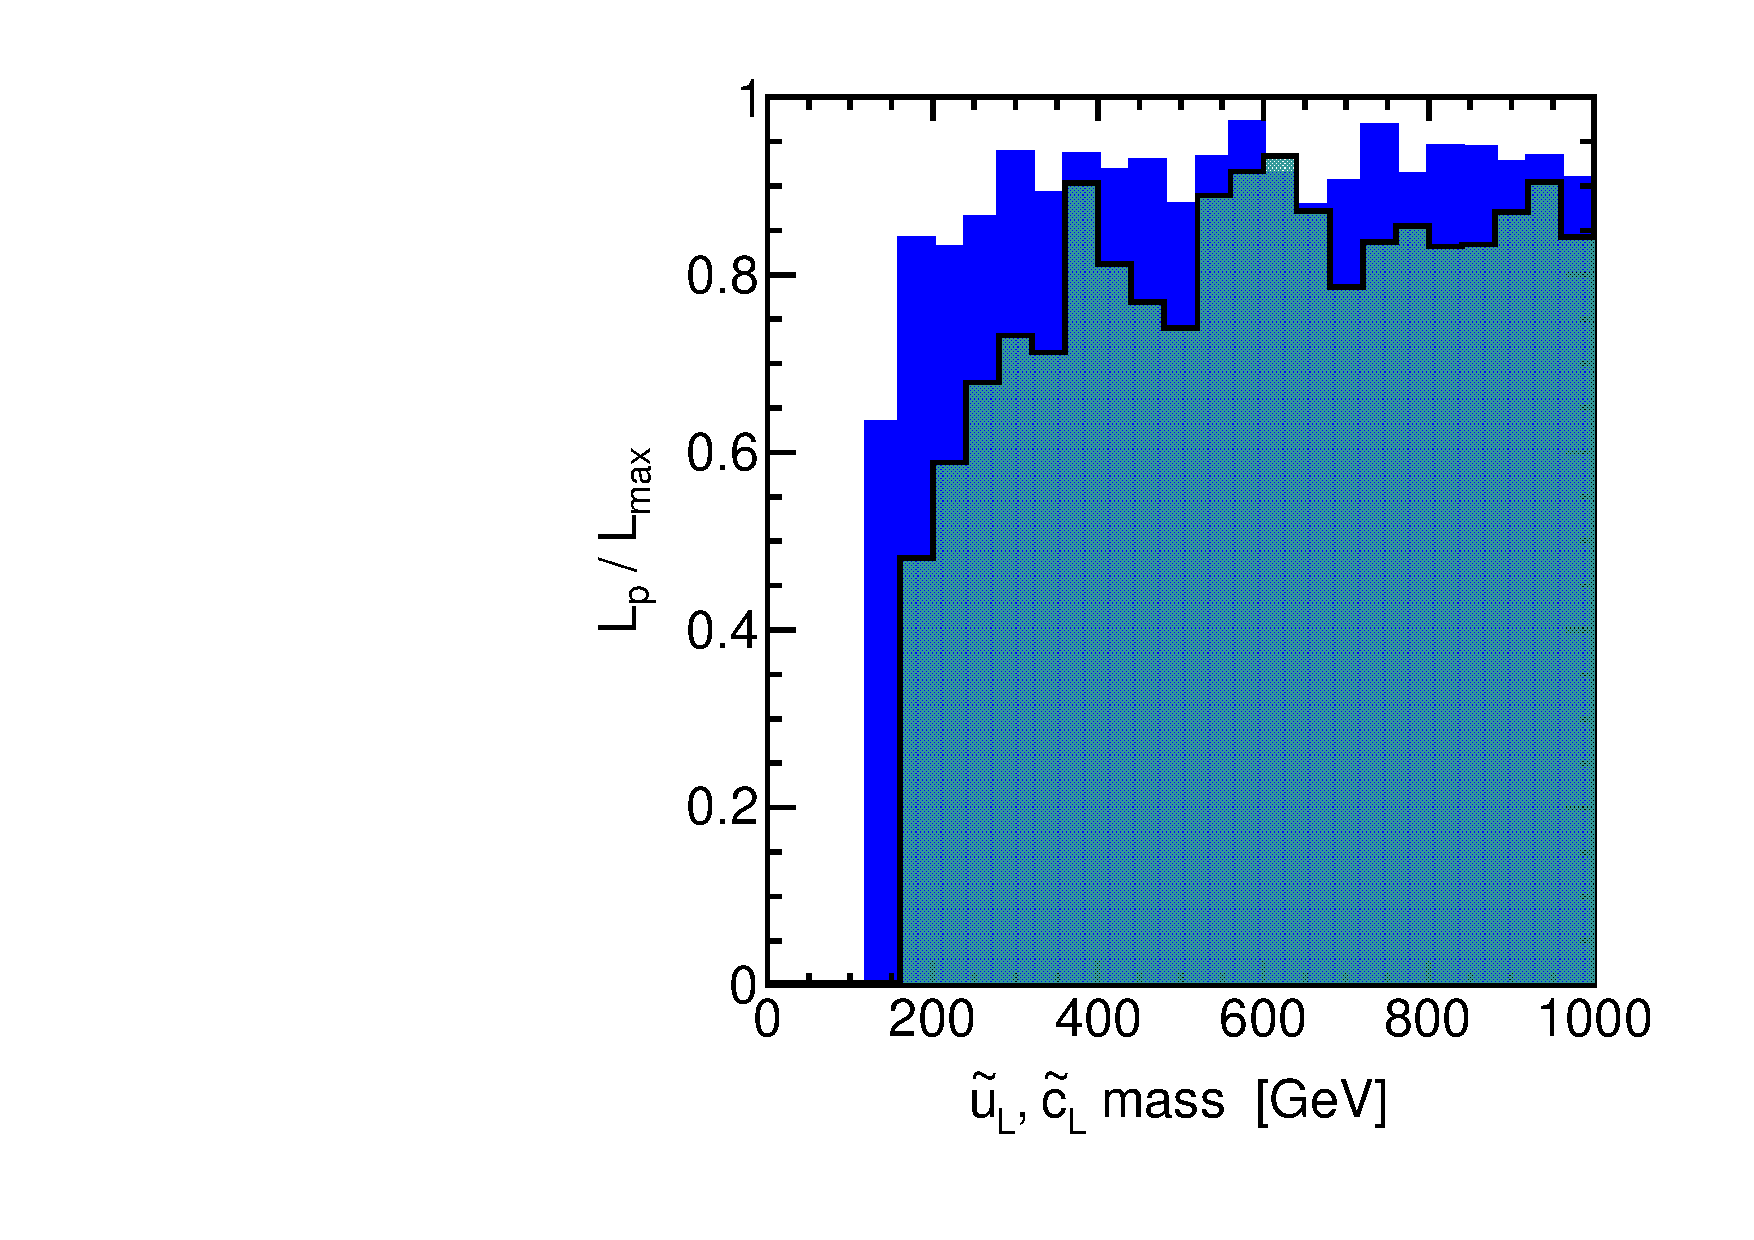
\includegraphics[height=5.5cm]{figs/fig_u_L.pdf} 
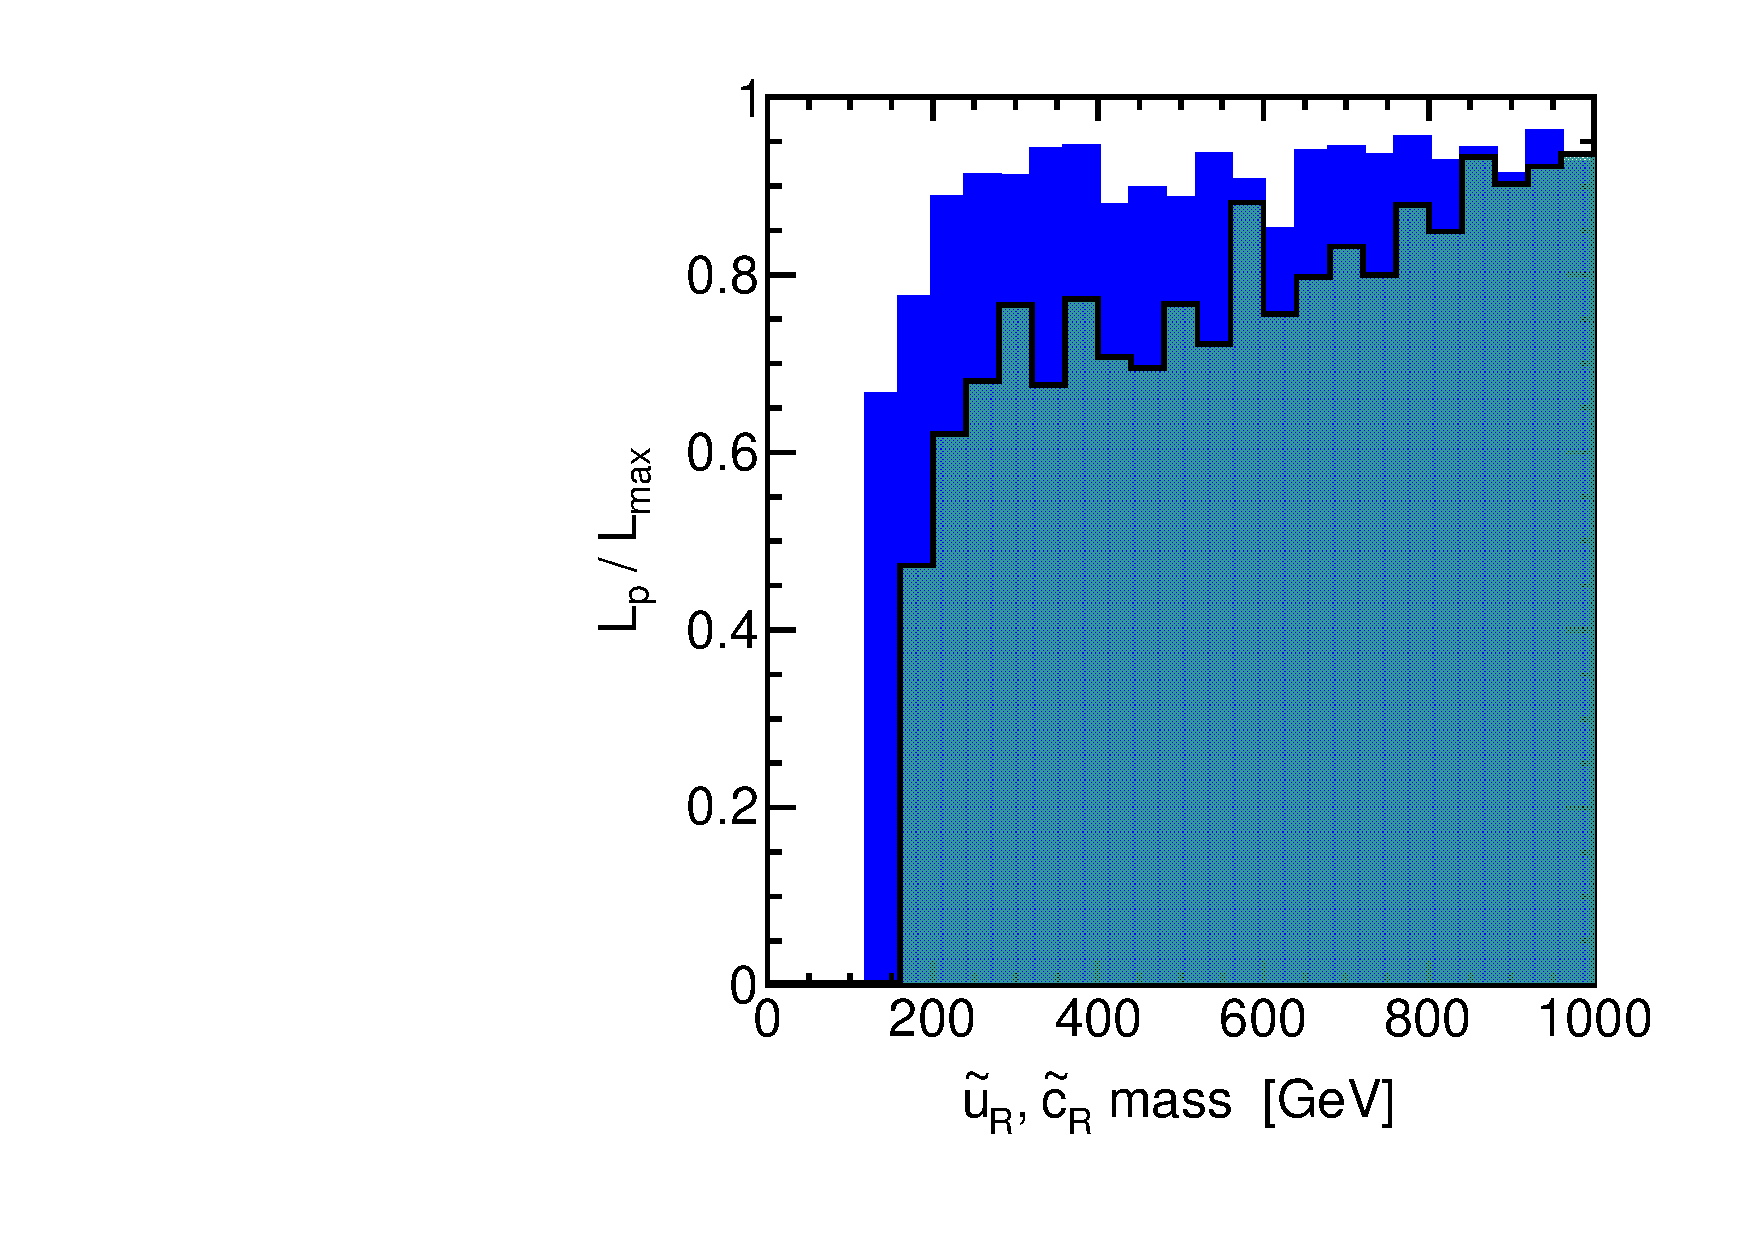
\includegraphics[height=5.5cm]{figs/fig_u_R.pdf} \\
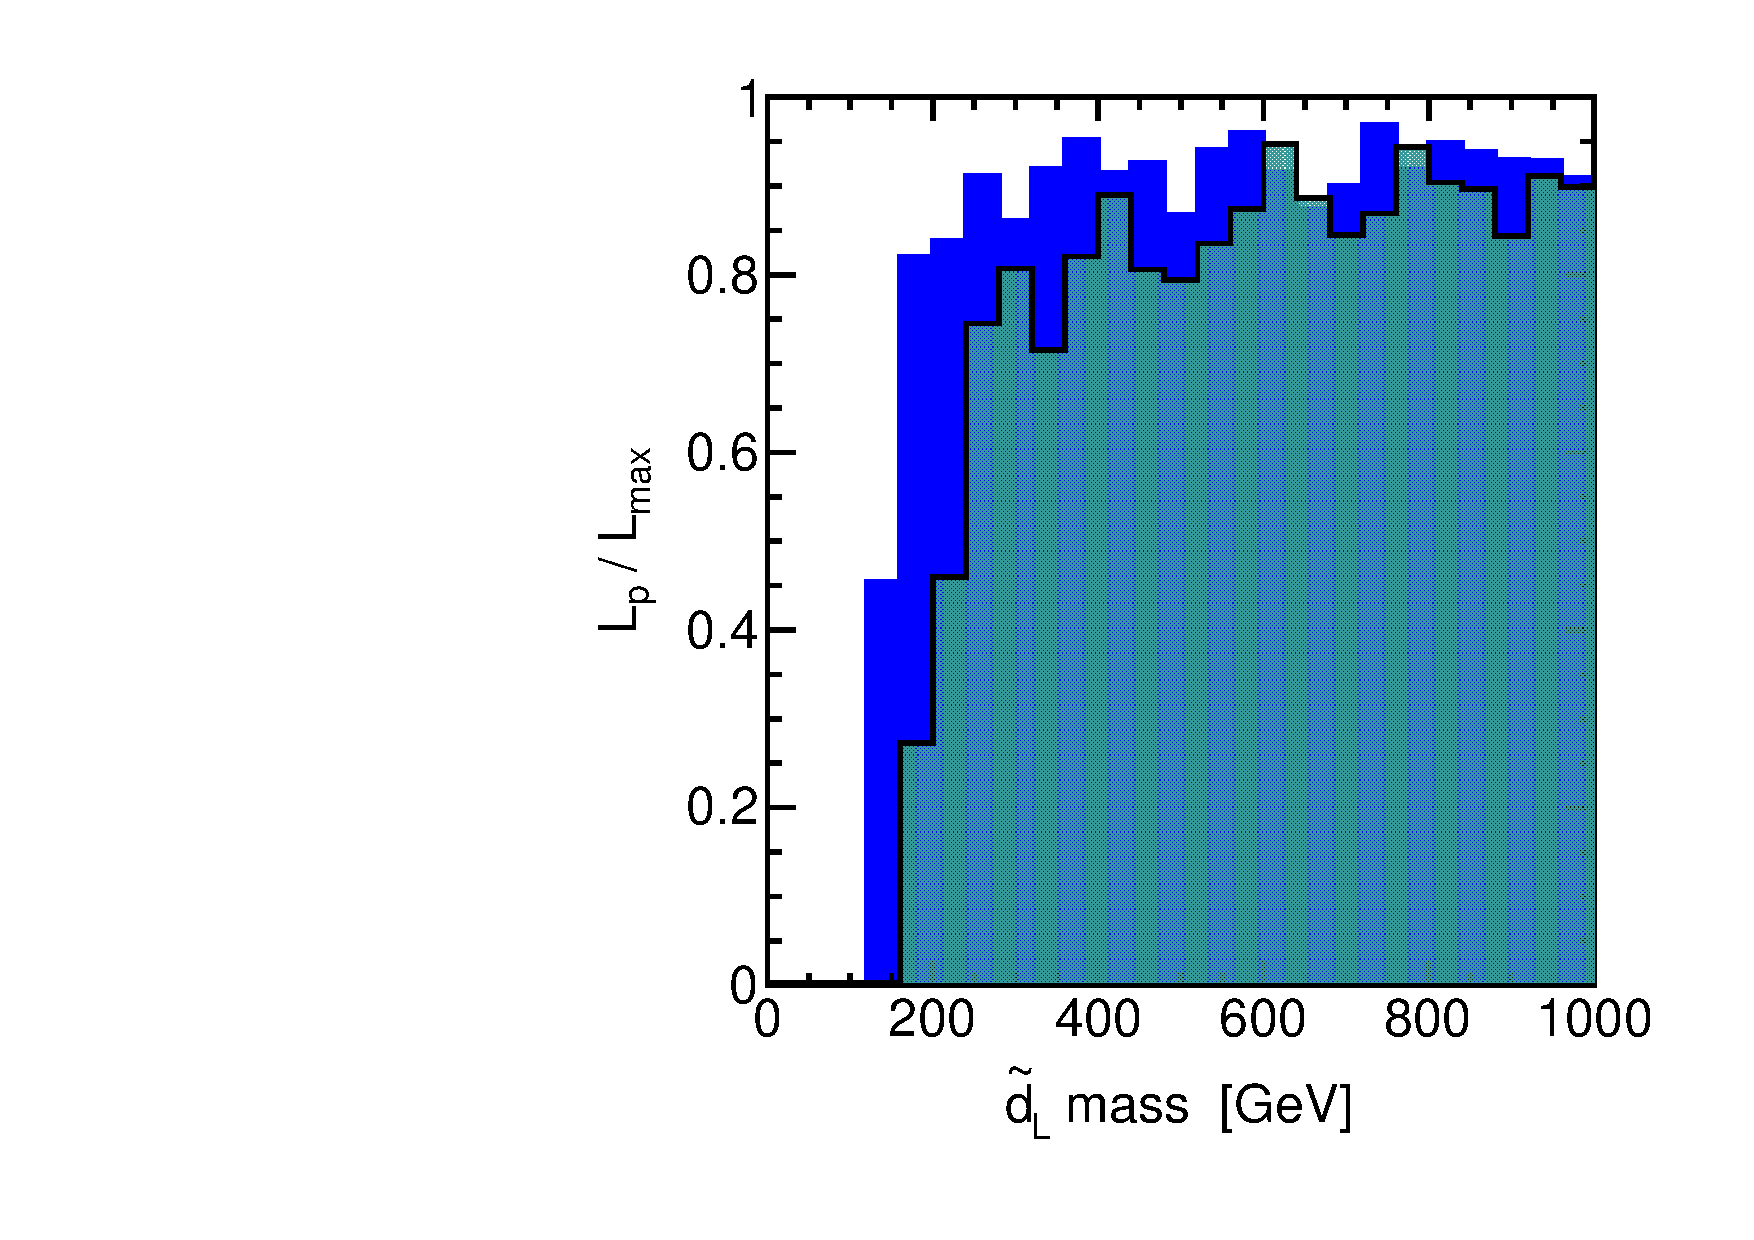
\includegraphics[height=5.5cm]{figs/fig_d_L.pdf} 
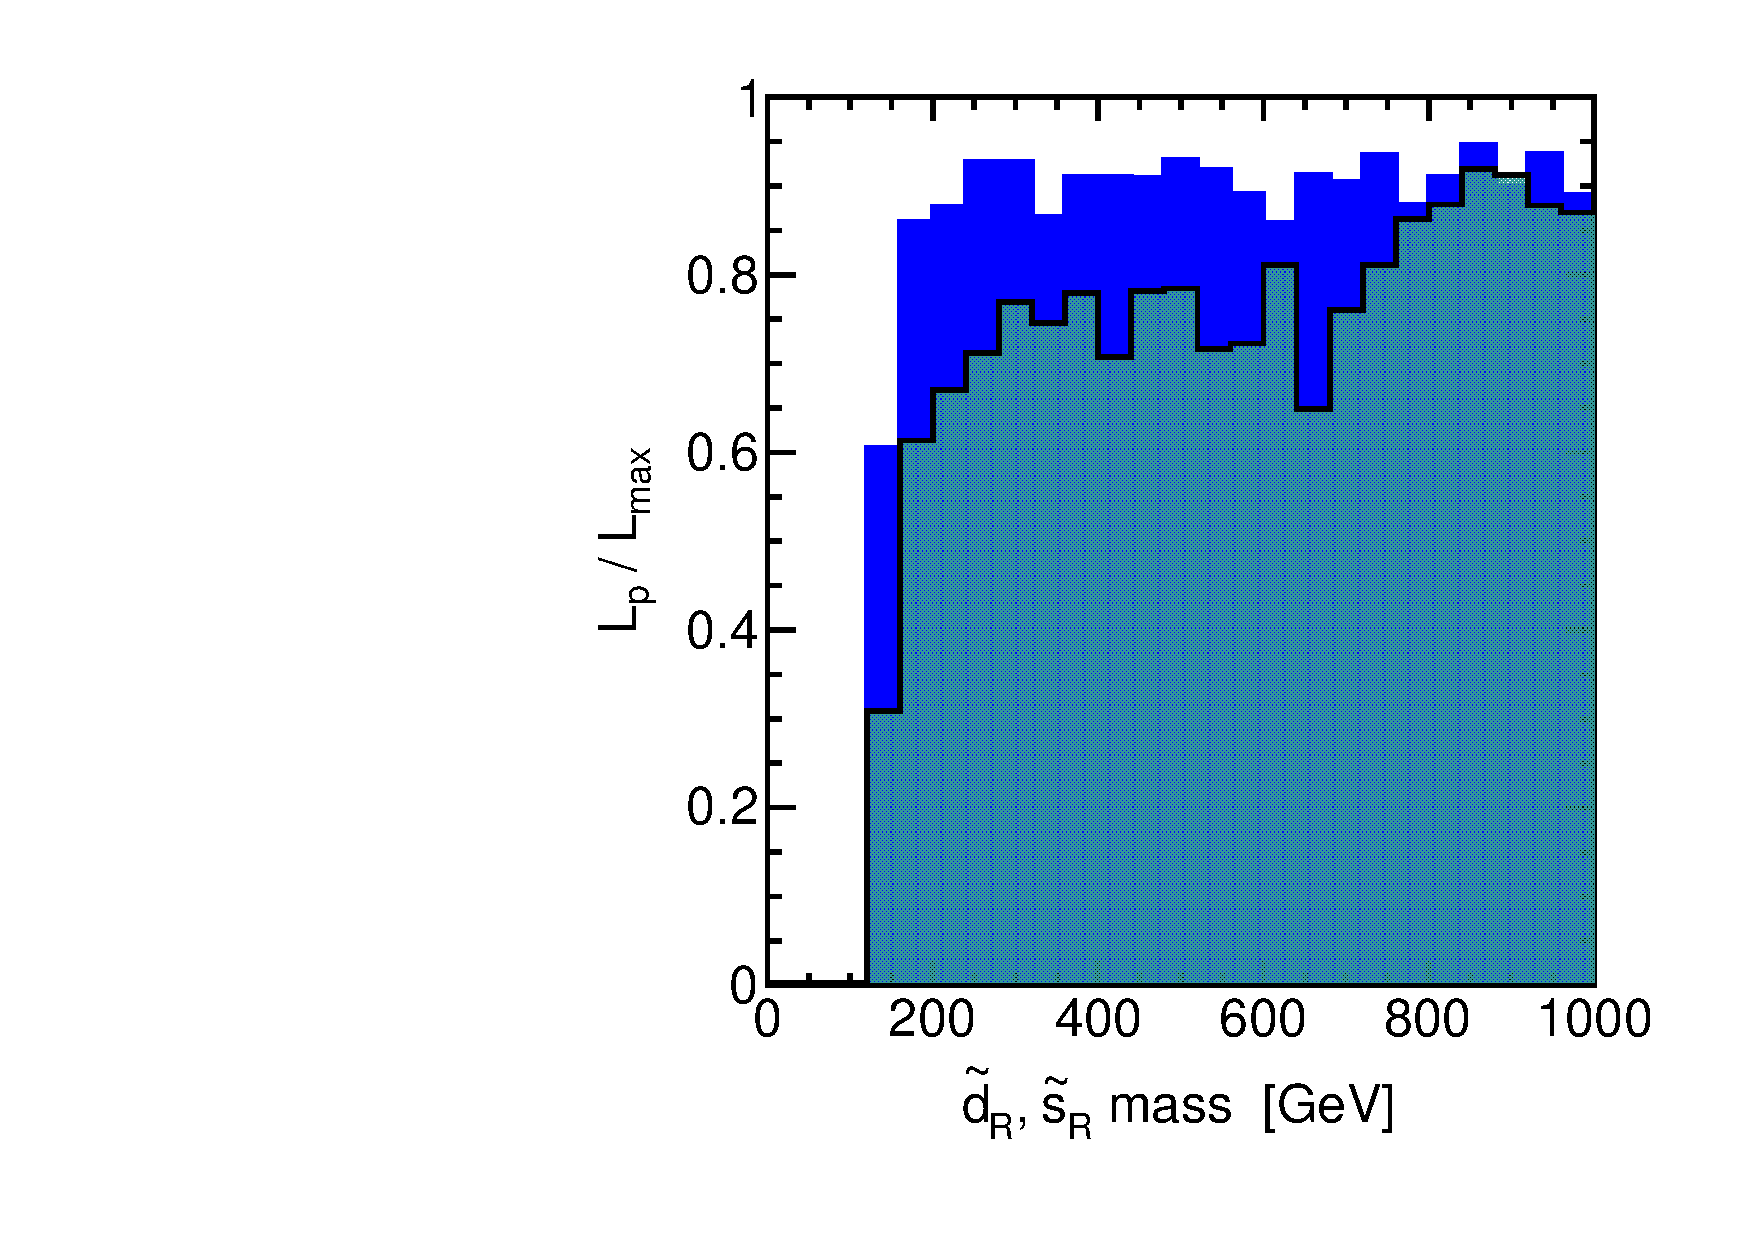
\includegraphics[height=5.5cm]{figs/fig_d_R.pdf} \\
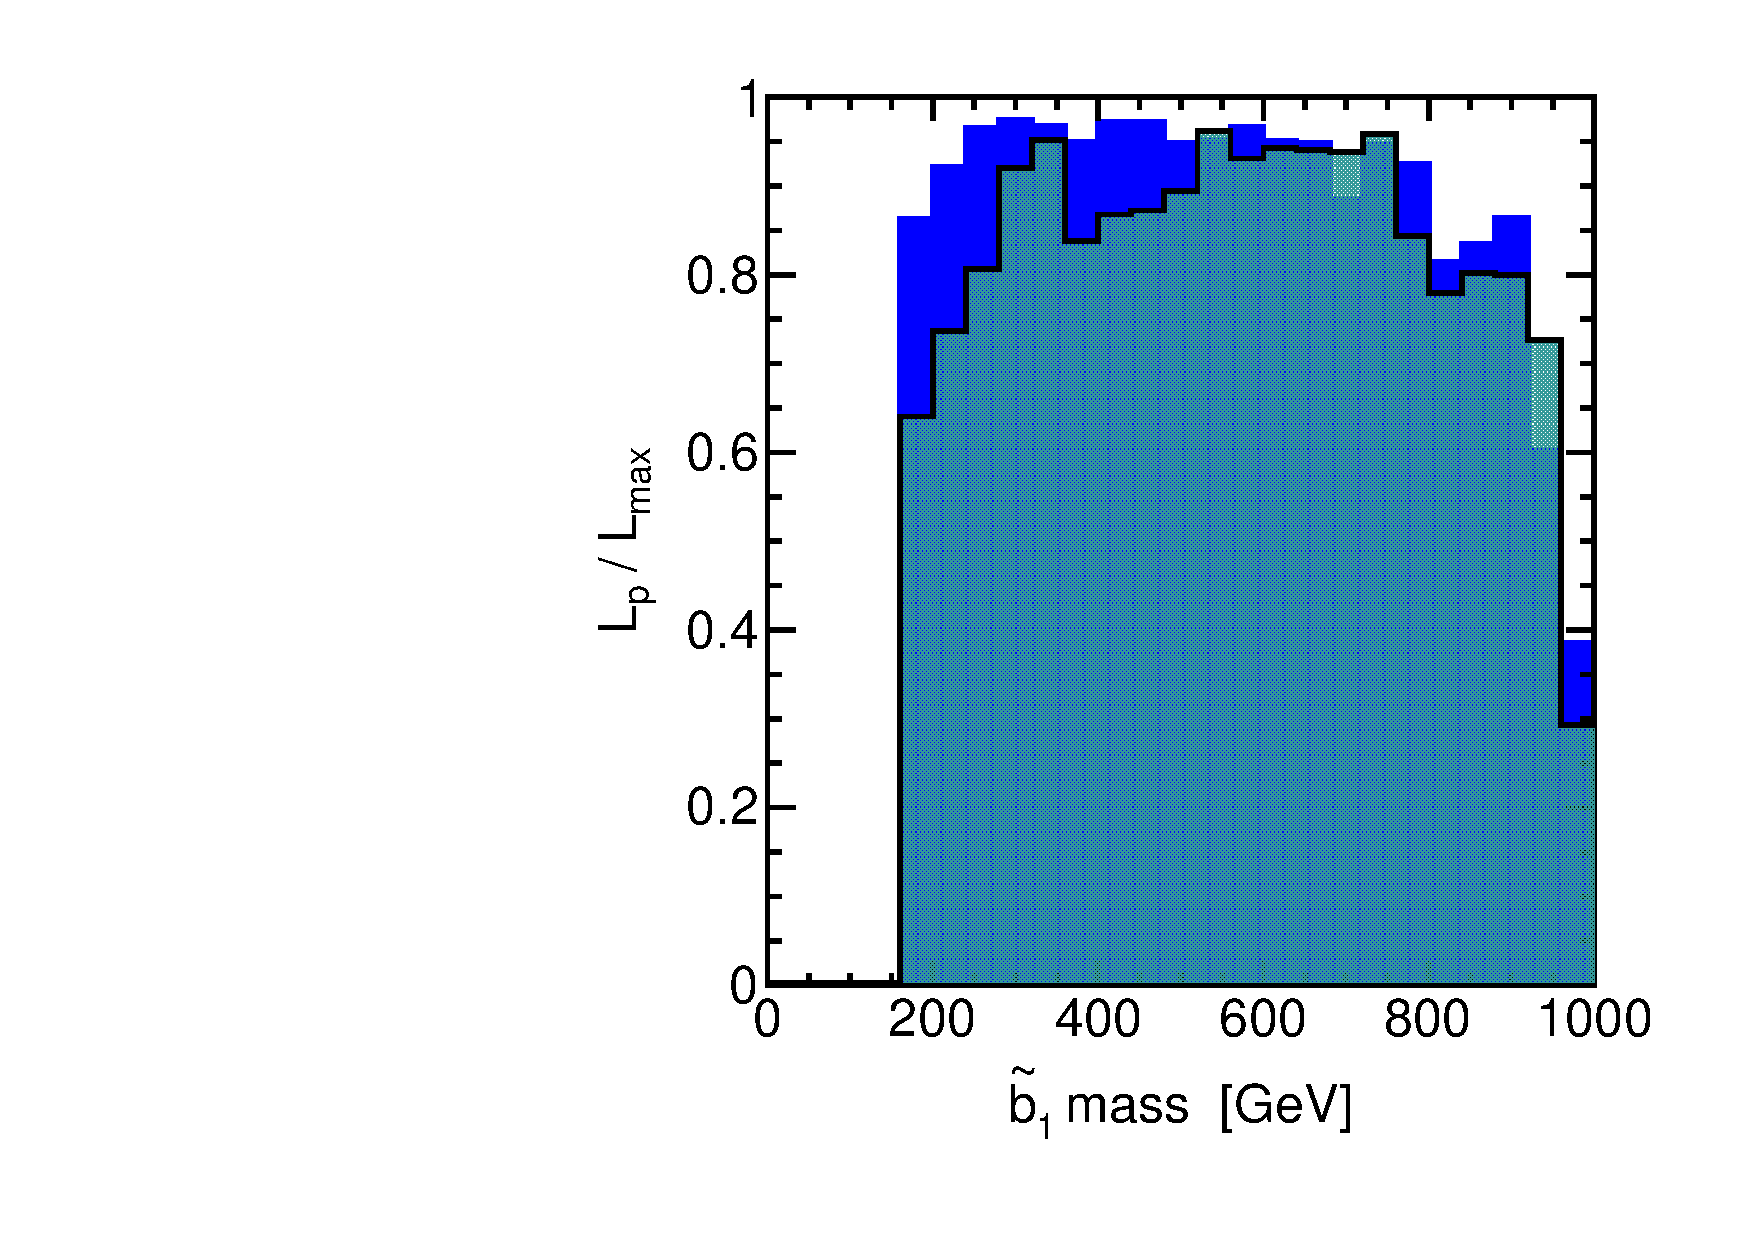
\includegraphics[height=5.5cm]{figs/fig_b_1.pdf} 
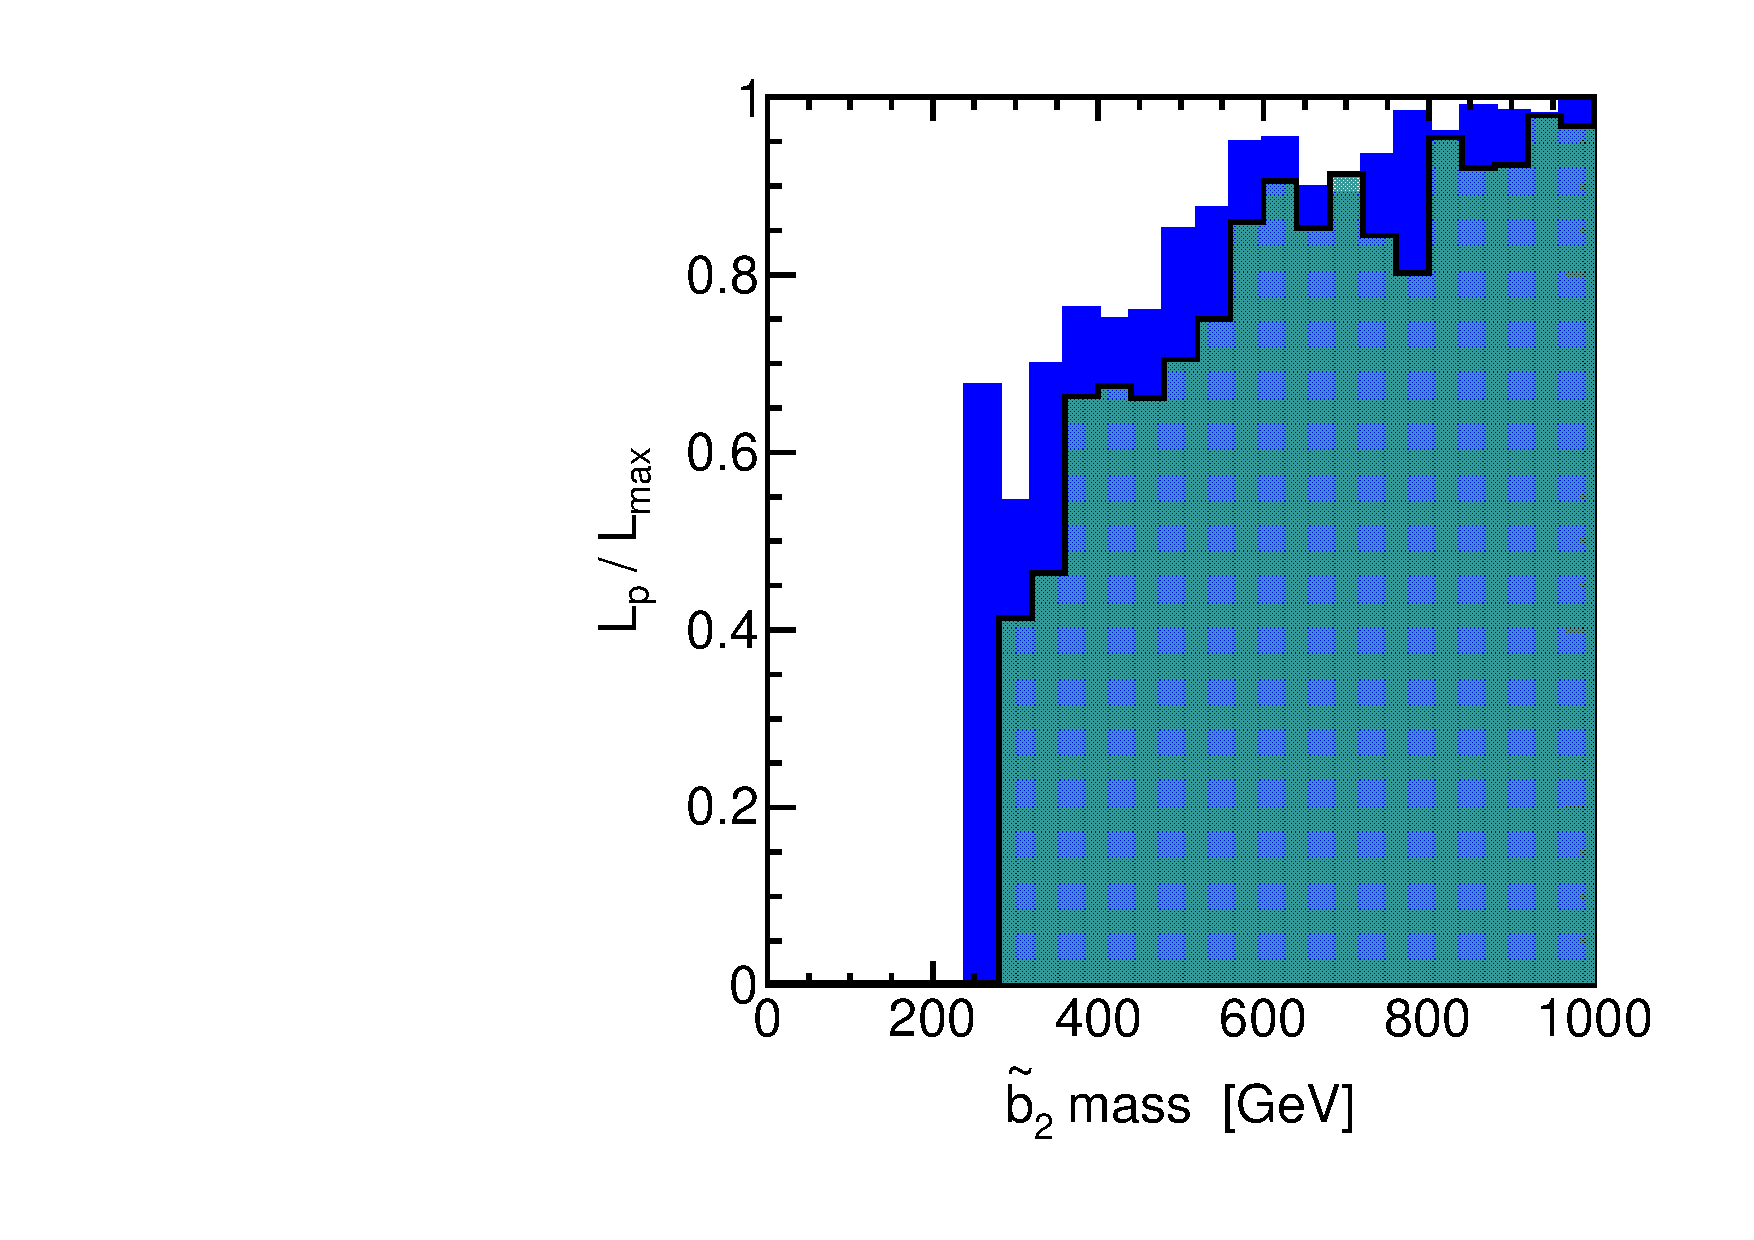
\includegraphics[height=5.5cm]{figs/fig_b_2.pdf} \\
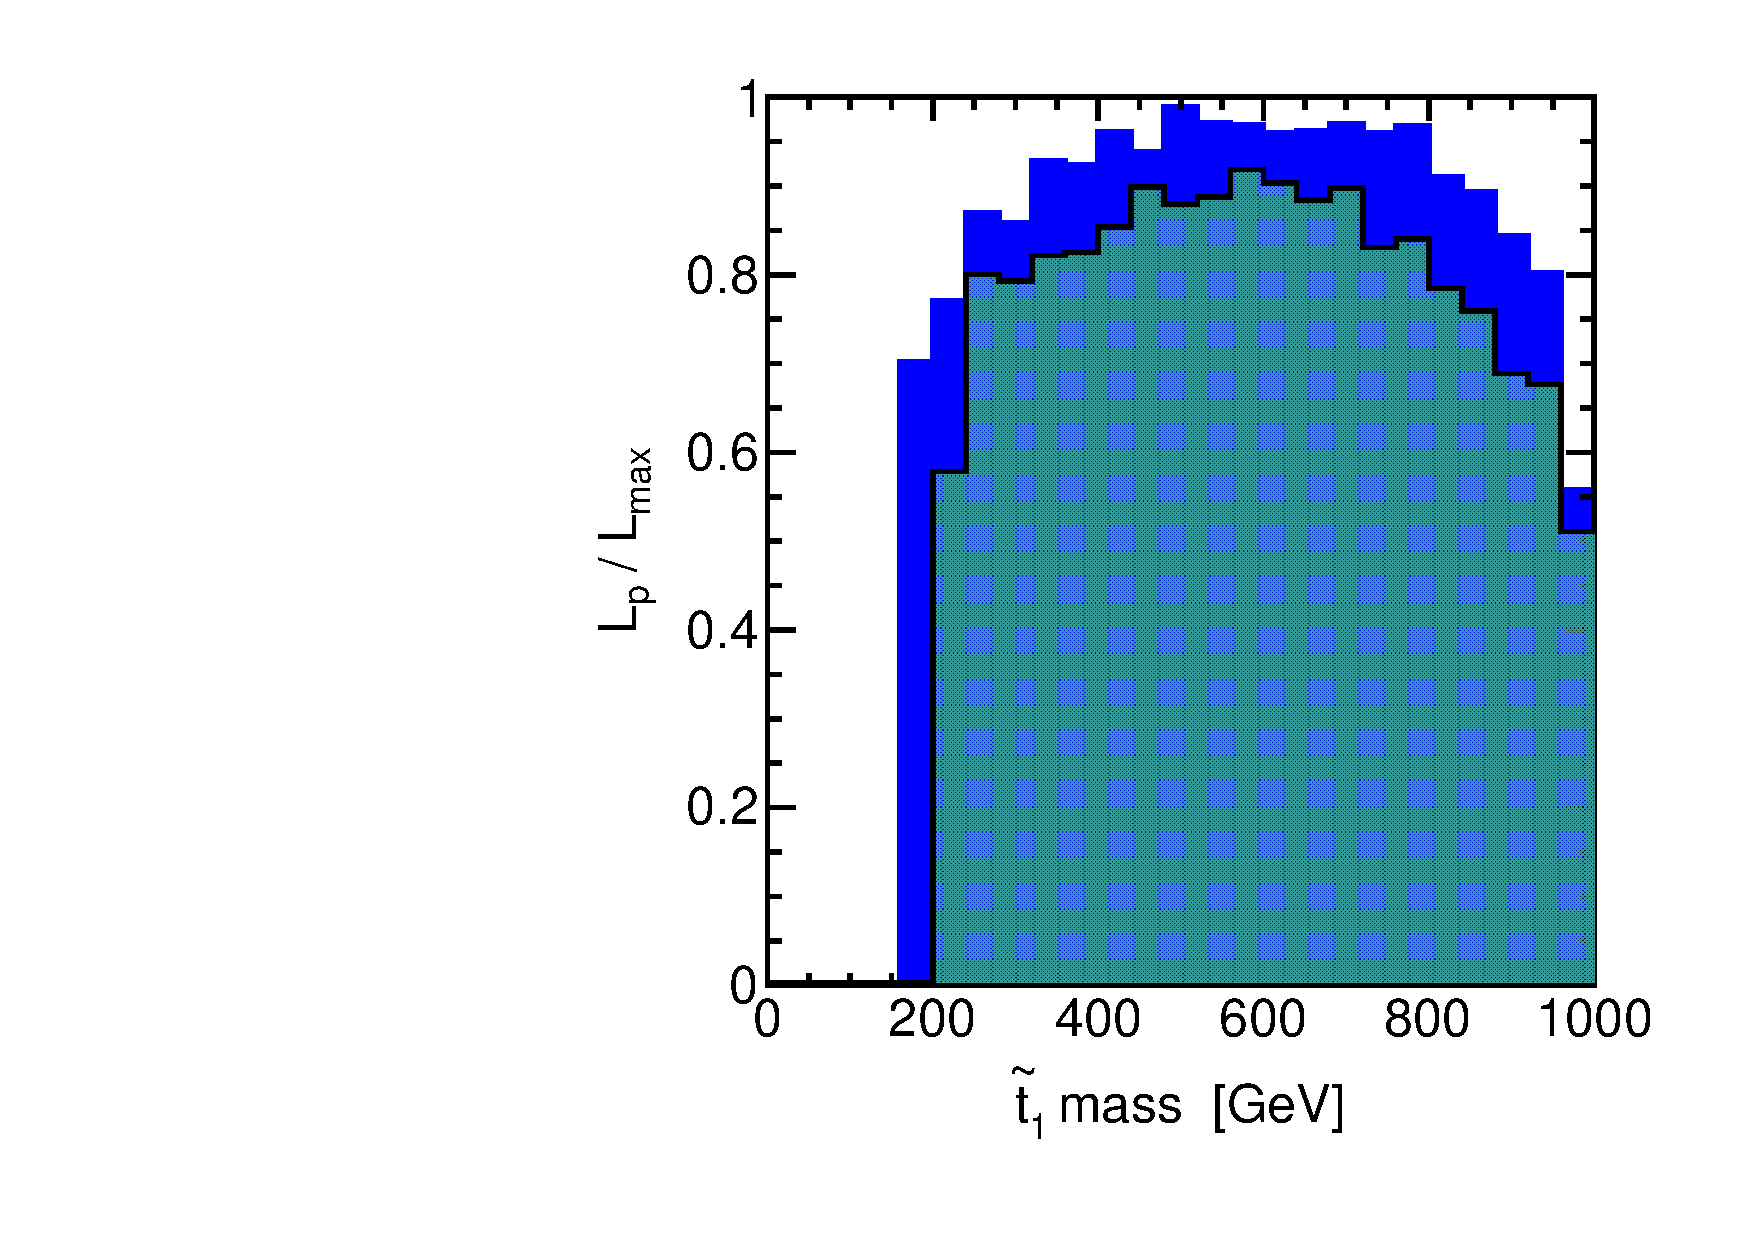
\includegraphics[height=5.5cm]{figs/fig_t_1.pdf} 
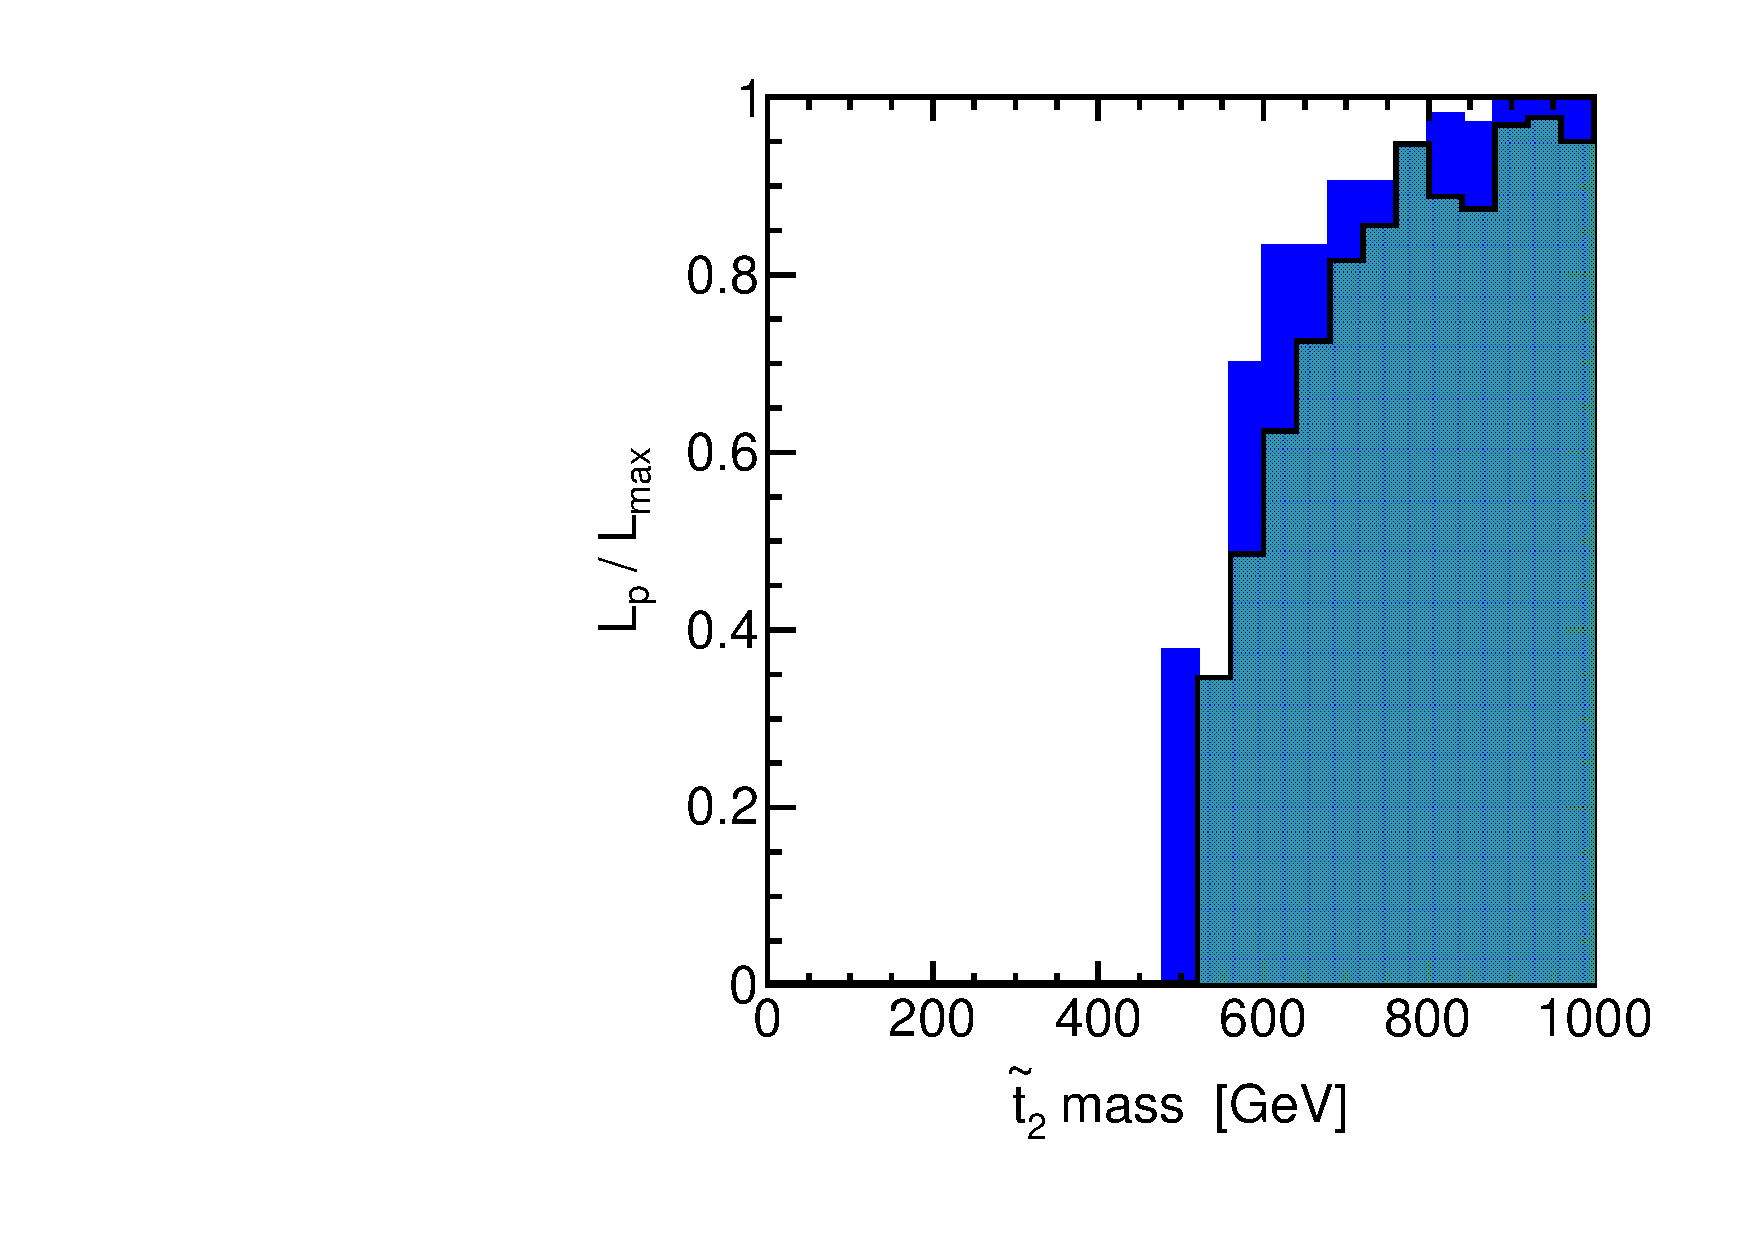
\includegraphics[height=5.5cm]{figs/fig_t_2.pdf} \\
\caption{Ratios of profile likelihood $L_p$ to maximum likelihood $L_{max}$ shown for squark masses.  The colored and shaded histograms show the distributions before and after the inclusion of the CMS results.}
\label{fig:LRwcms_sq}
\end{center}
\end{figure}


\begin{figure}[htbp]
\begin{center}
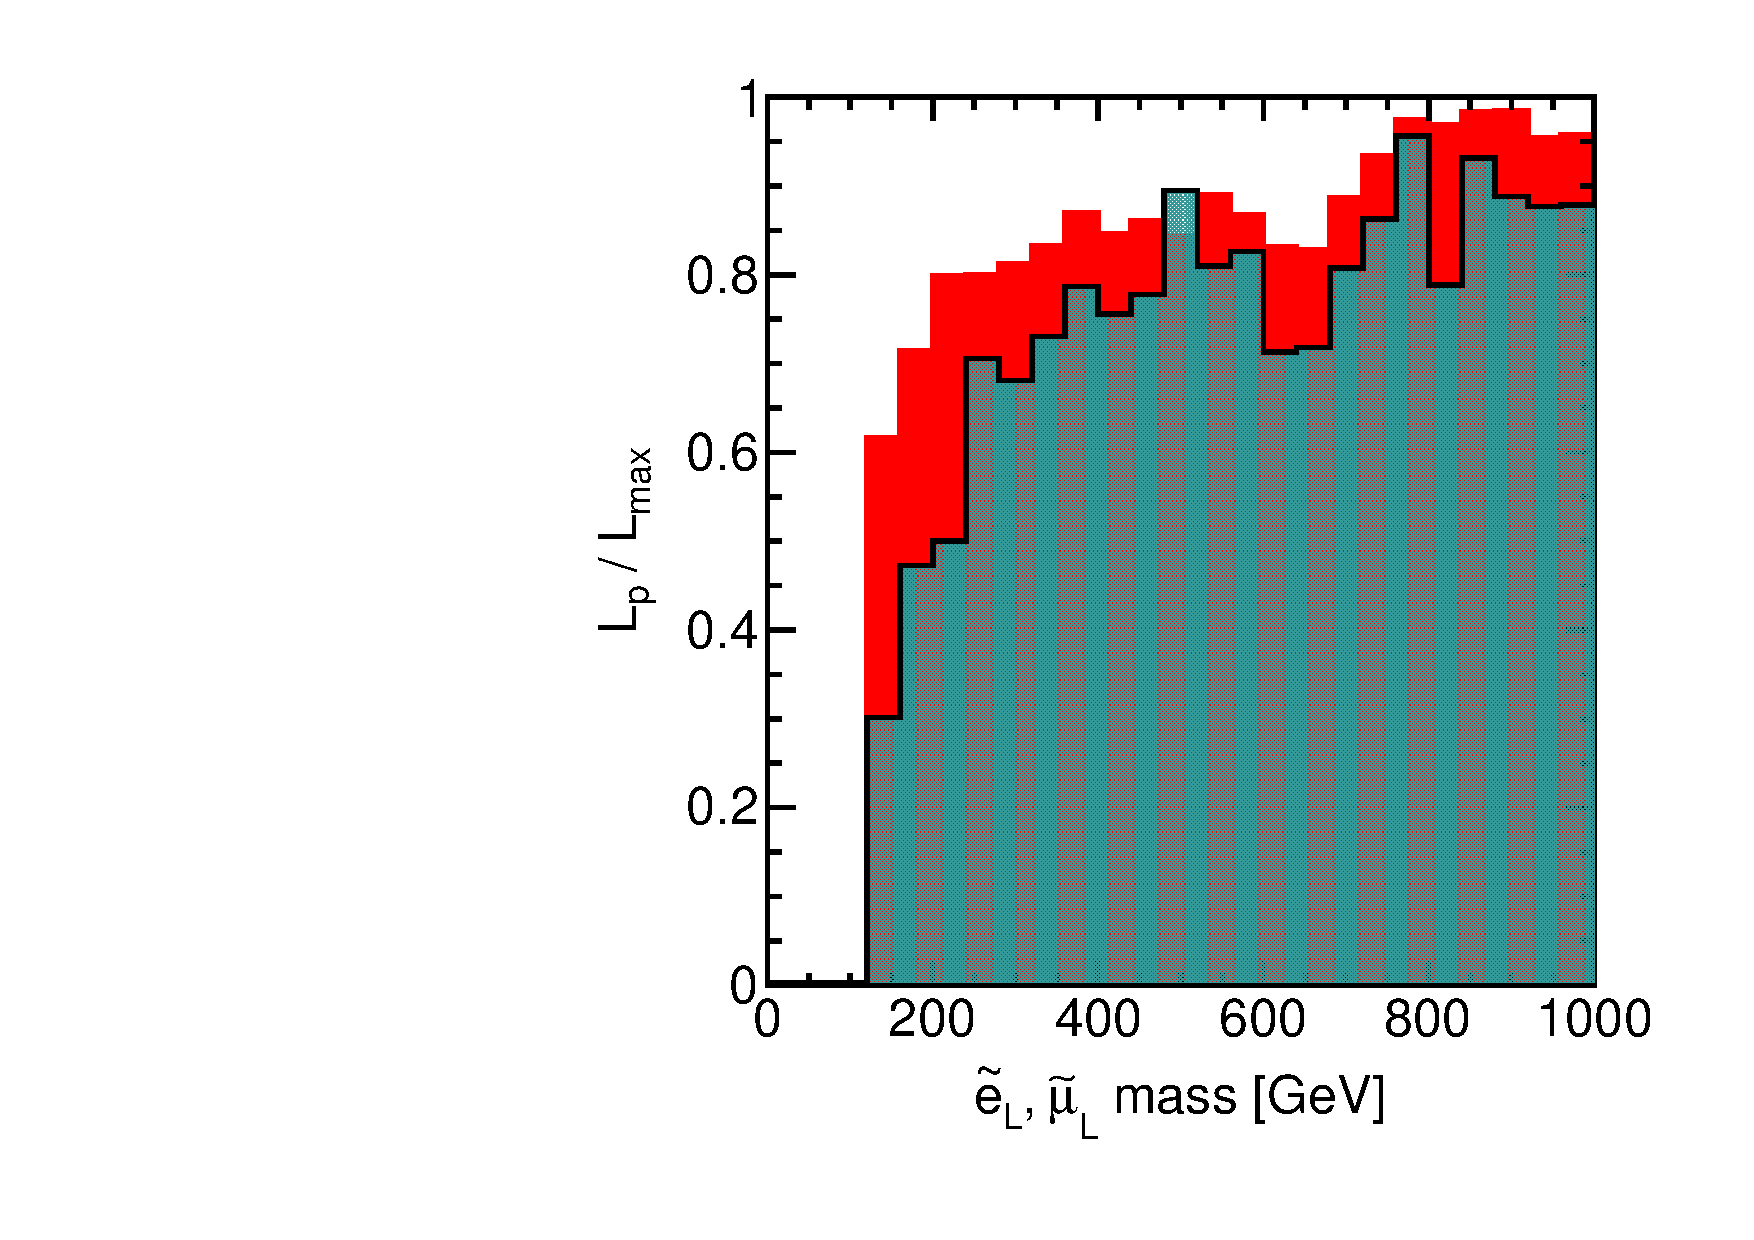
\includegraphics[height=5.5cm]{figs/fig_e_L.pdf} 
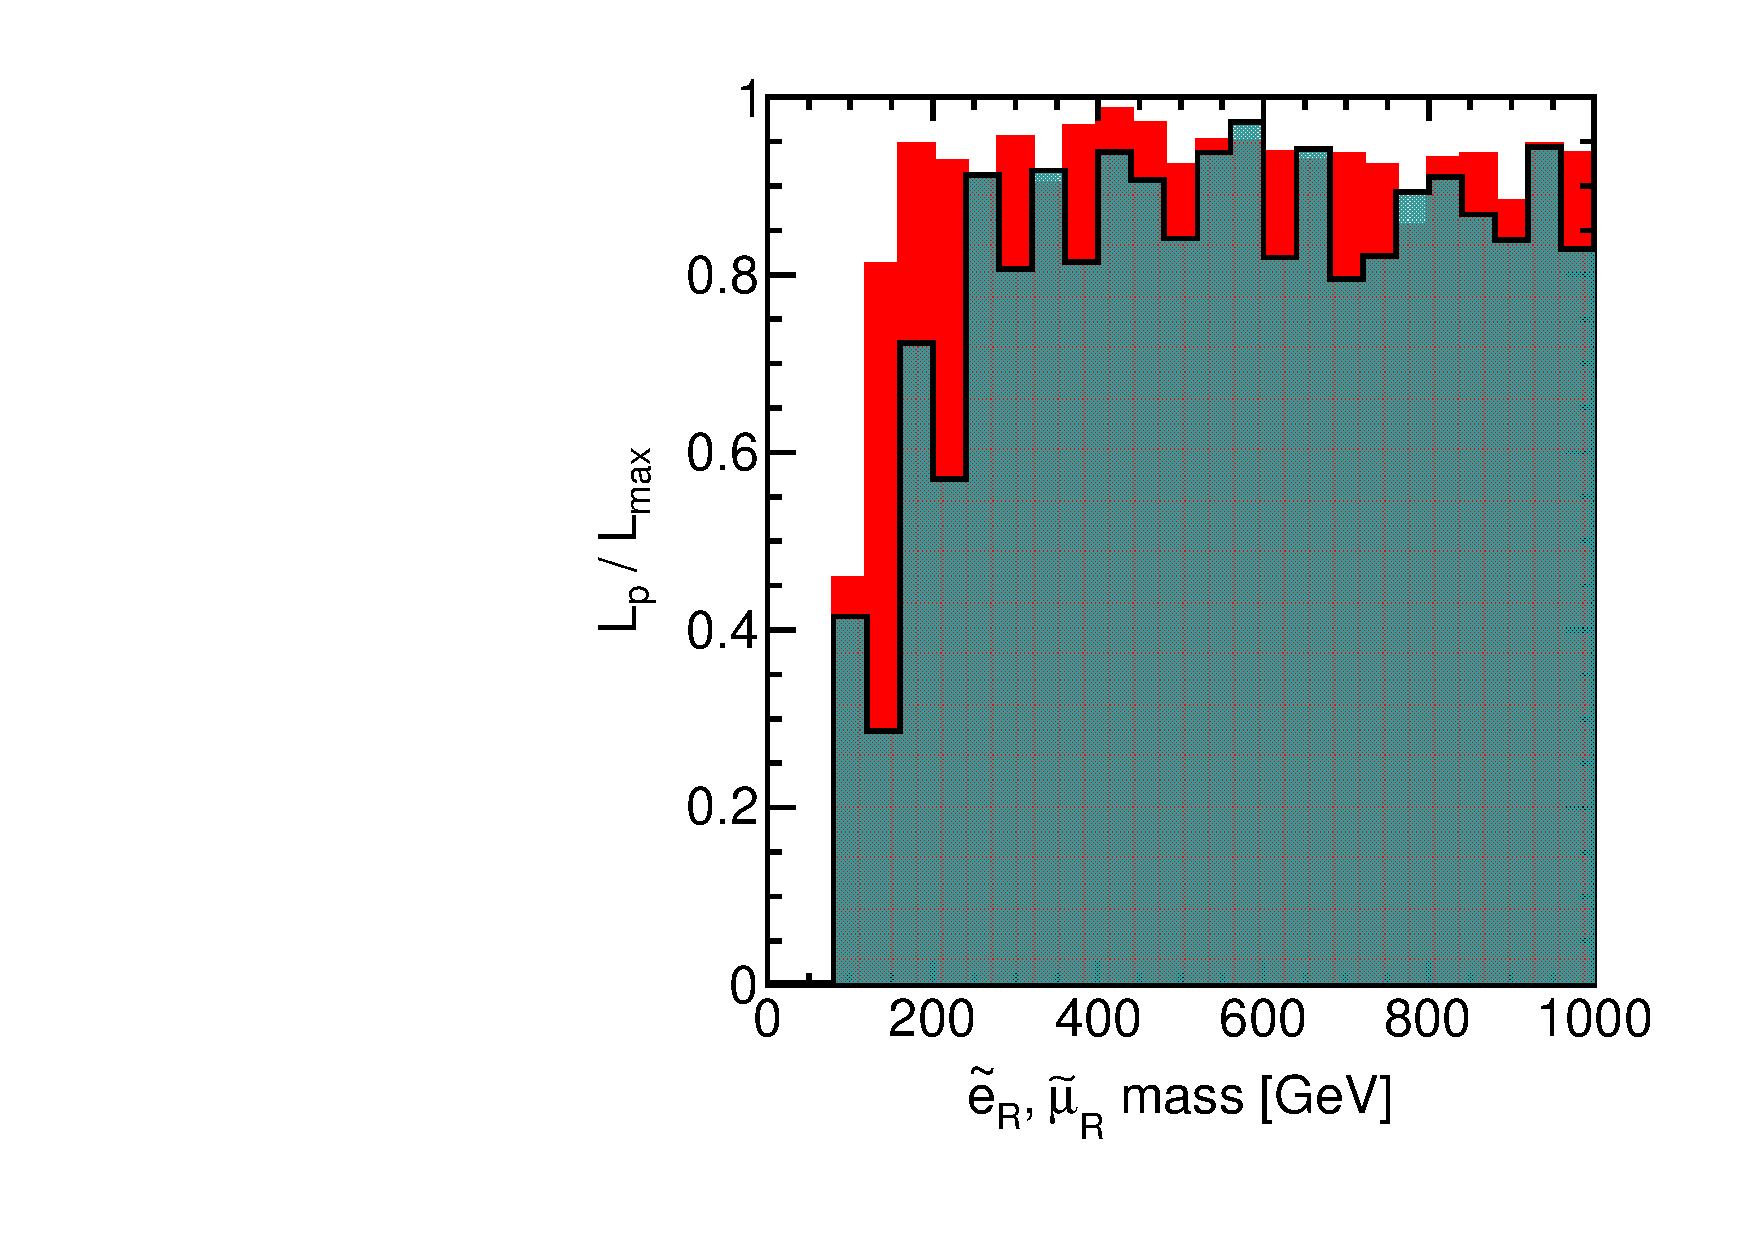
\includegraphics[height=5.5cm]{figs/fig_e_R.pdf} \\
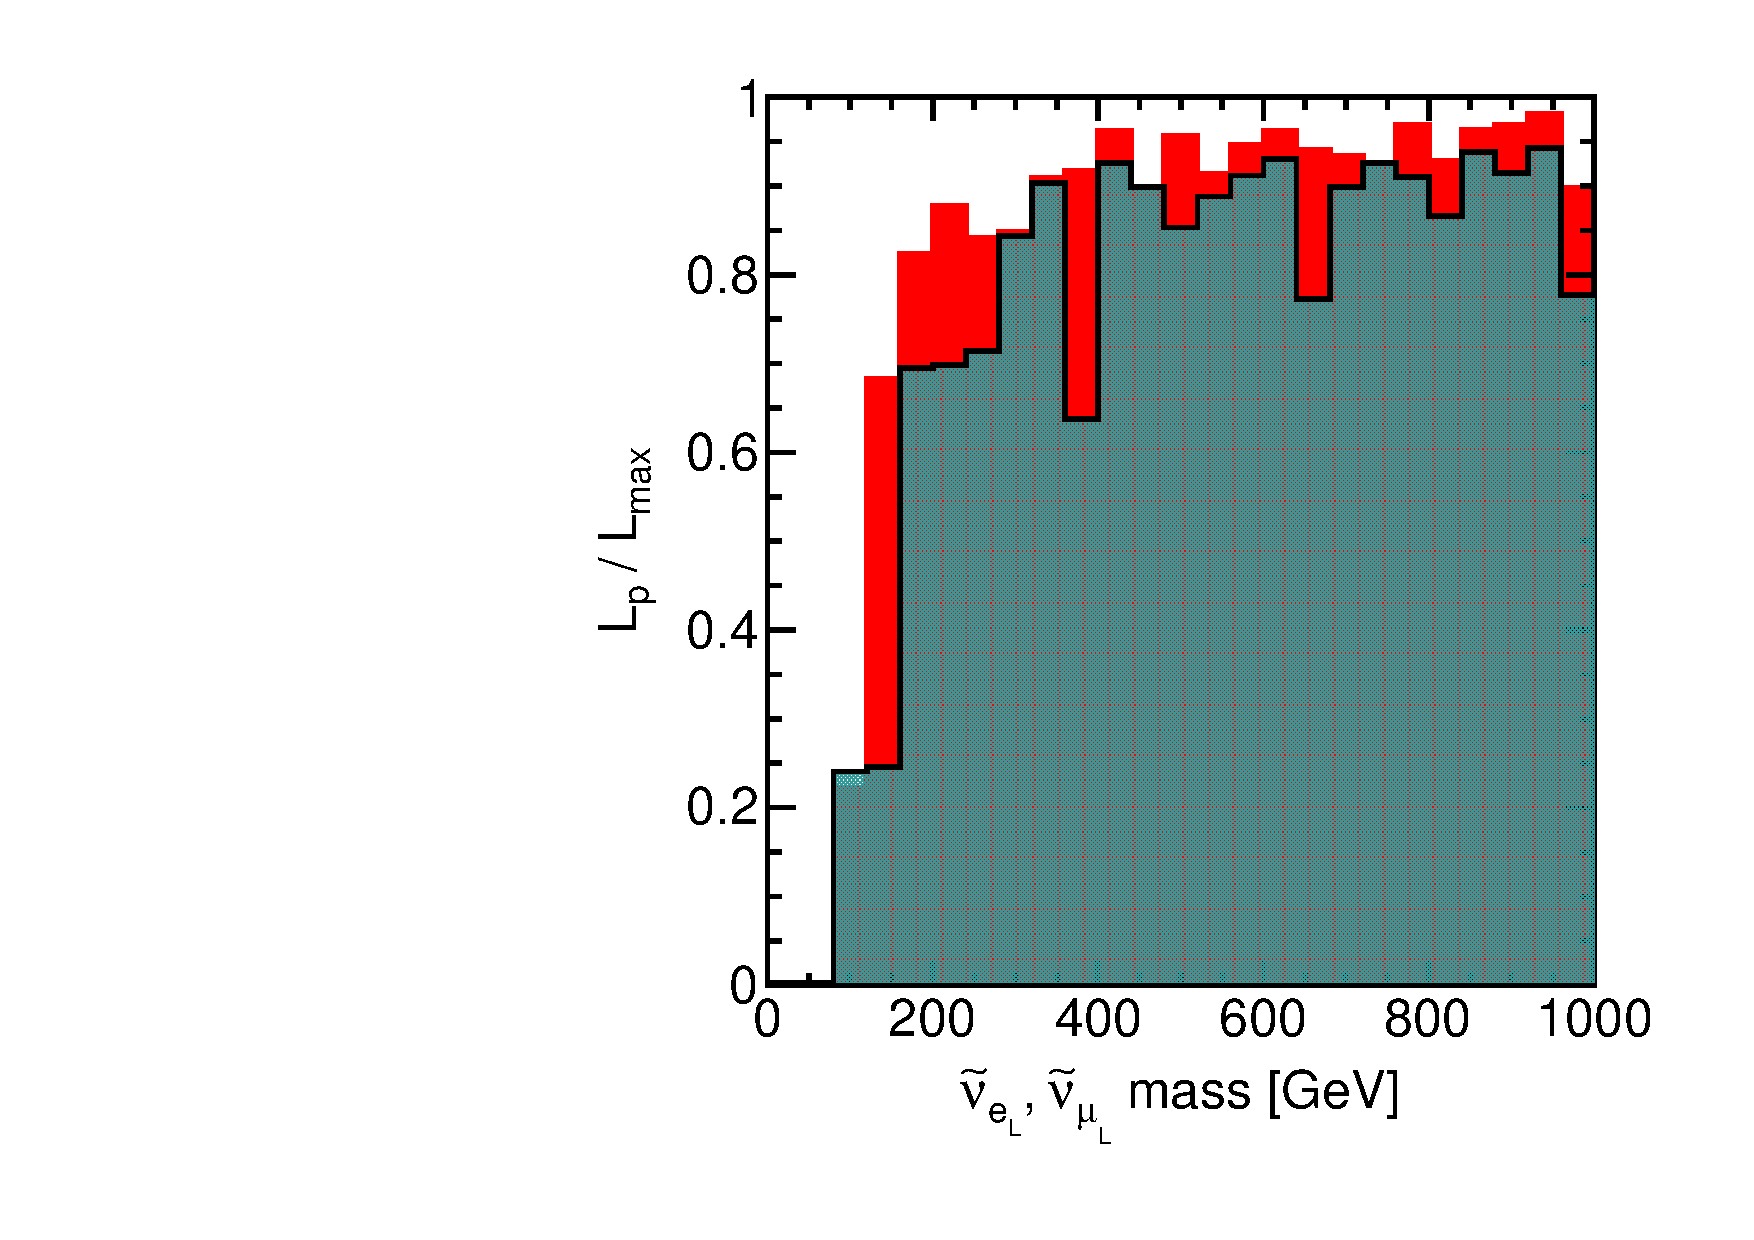
\includegraphics[height=5.5cm]{figs/fig_nu_e_L.pdf} 
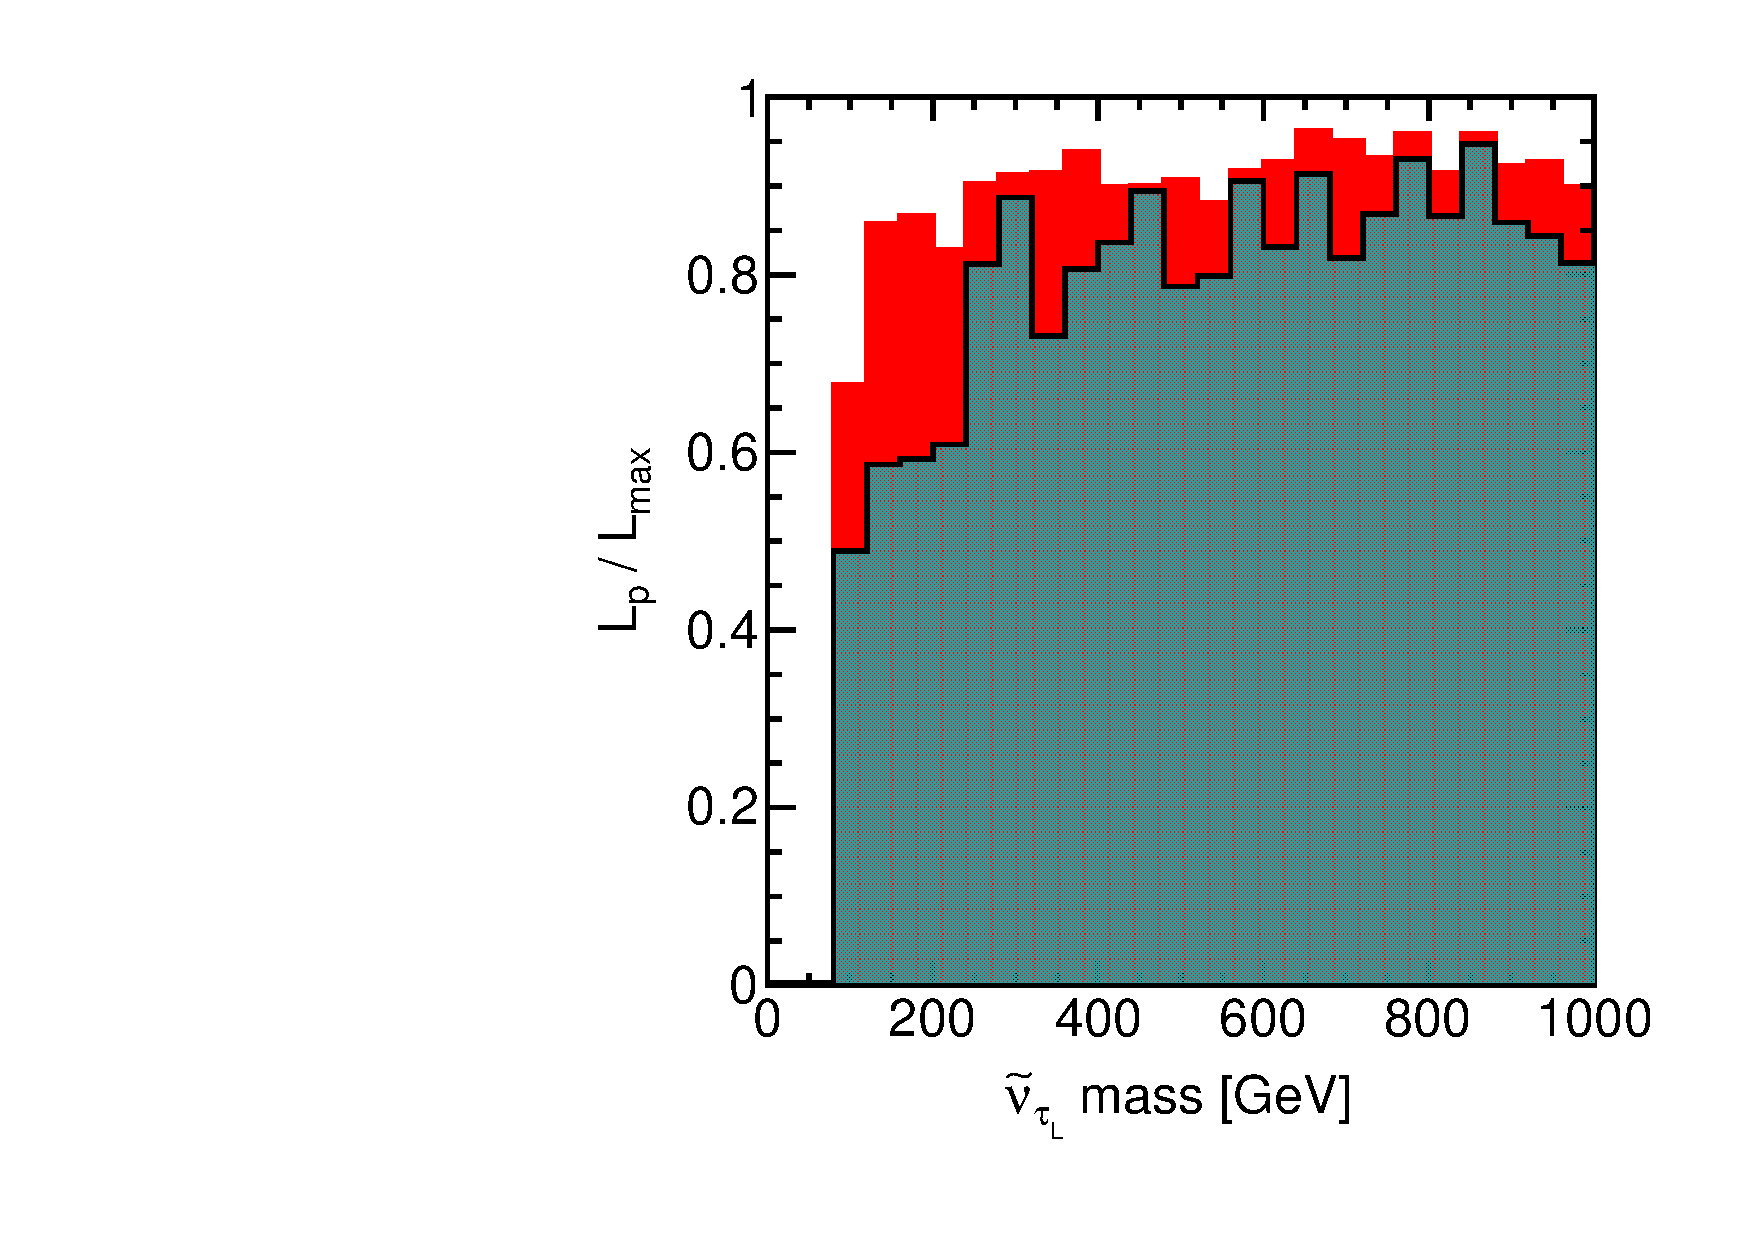
\includegraphics[height=5.5cm]{figs/fig_nu_tau_L.pdf} \\
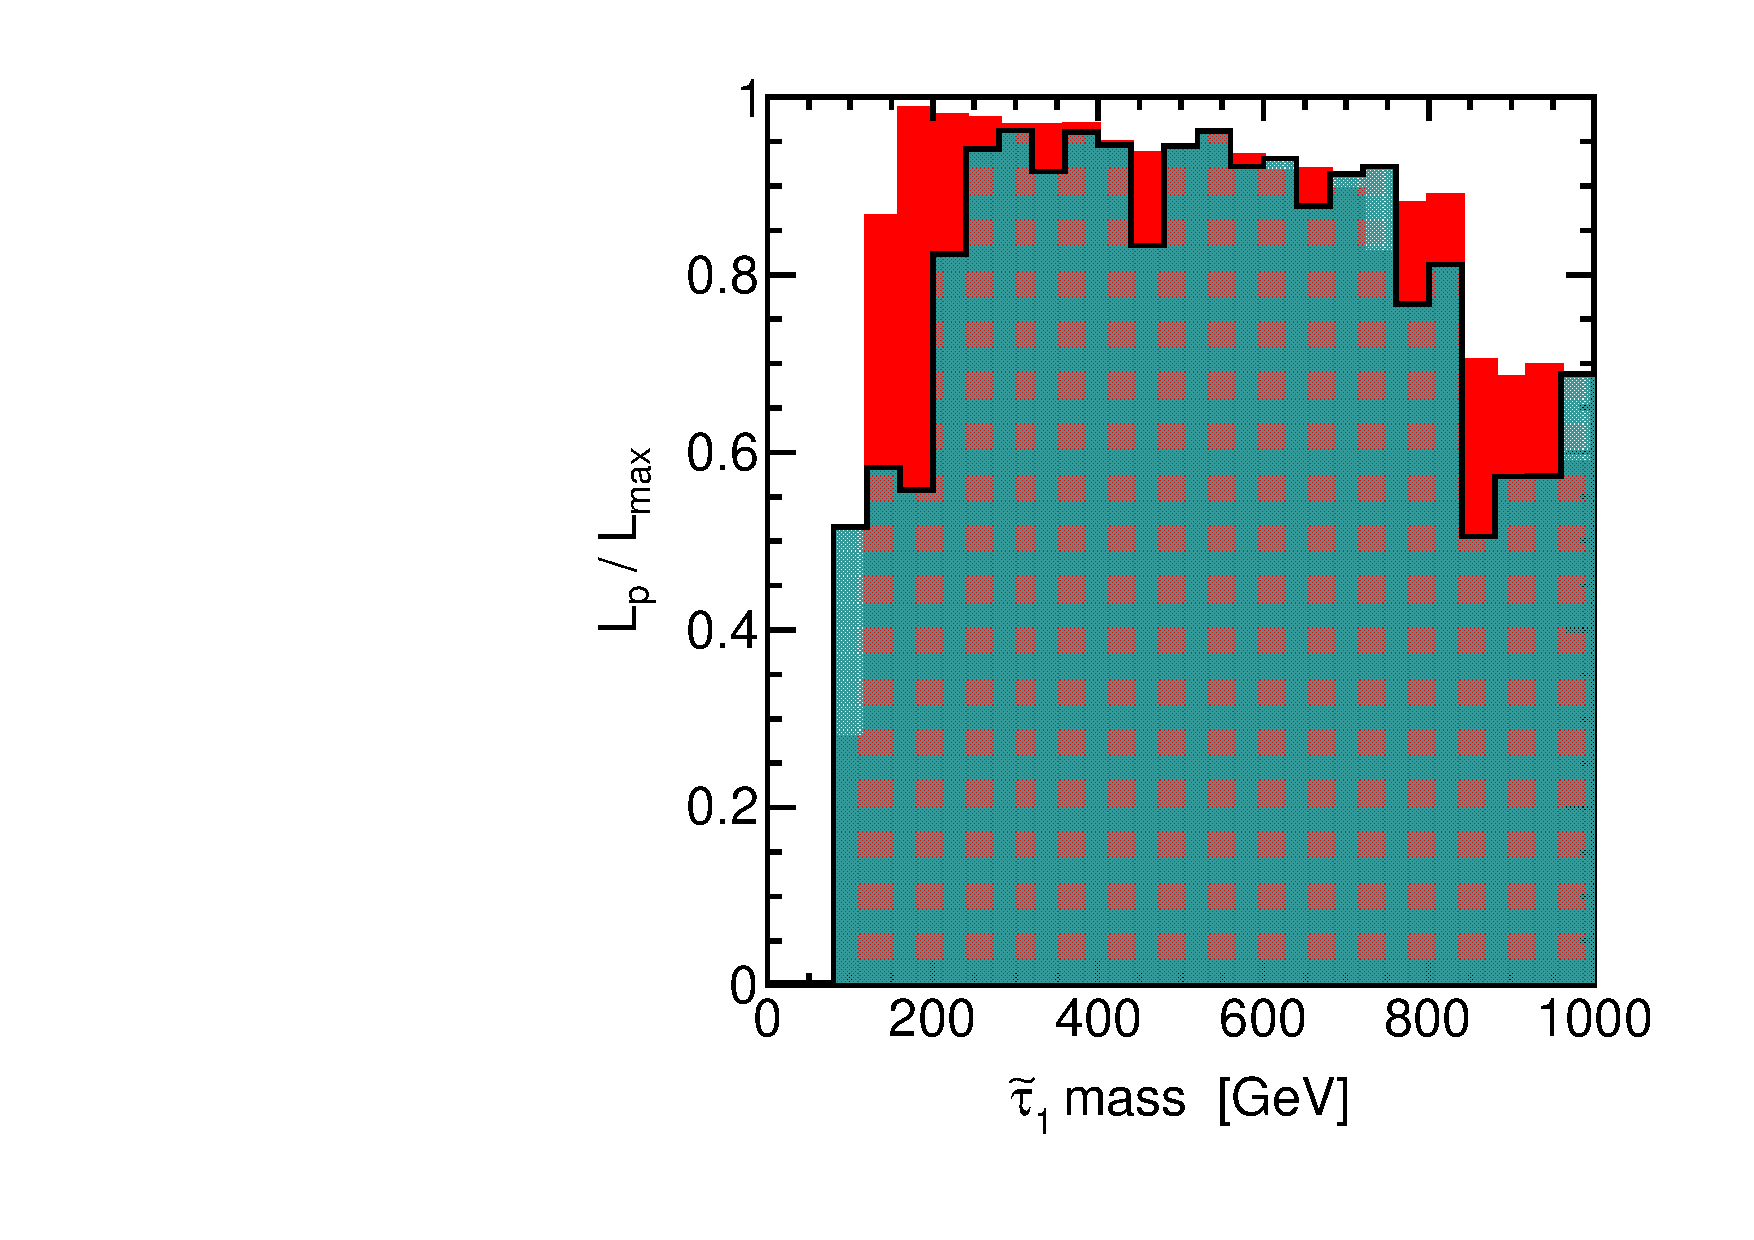
\includegraphics[height=5.5cm]{figs/fig_tau_1.pdf} 
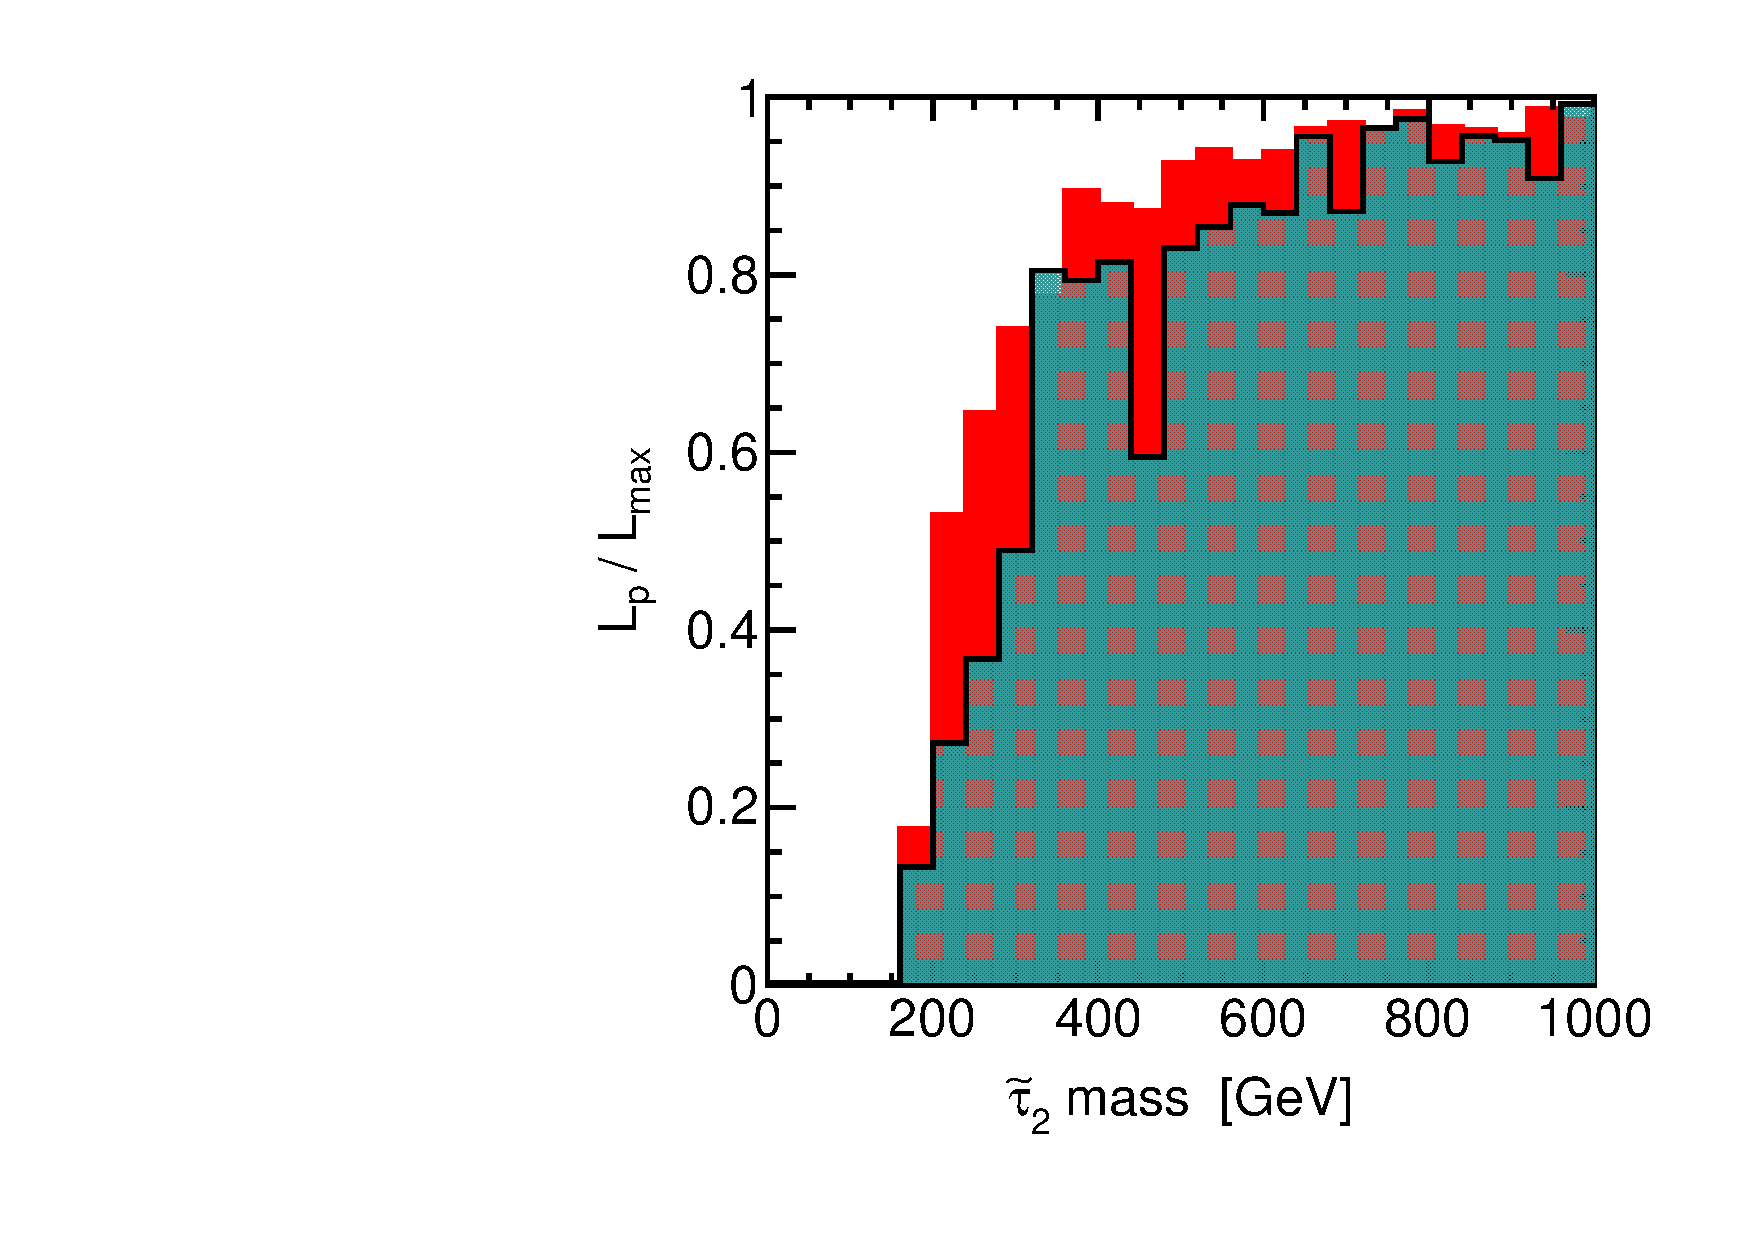
\includegraphics[height=5.5cm]{figs/fig_tau_2.pdf}
\caption{Ratios of profile likelihood $L_p$ to maximum likelihood $L_{max}$ shown for predictions for slepton masses.  The colored and shaded histograms show the distributions before and after the inclusion of the CMS results.}
\label{fig:LRwcms:sl}
\end{center}
\end{figure}

\begin{figure}[htbp]
\begin{center}
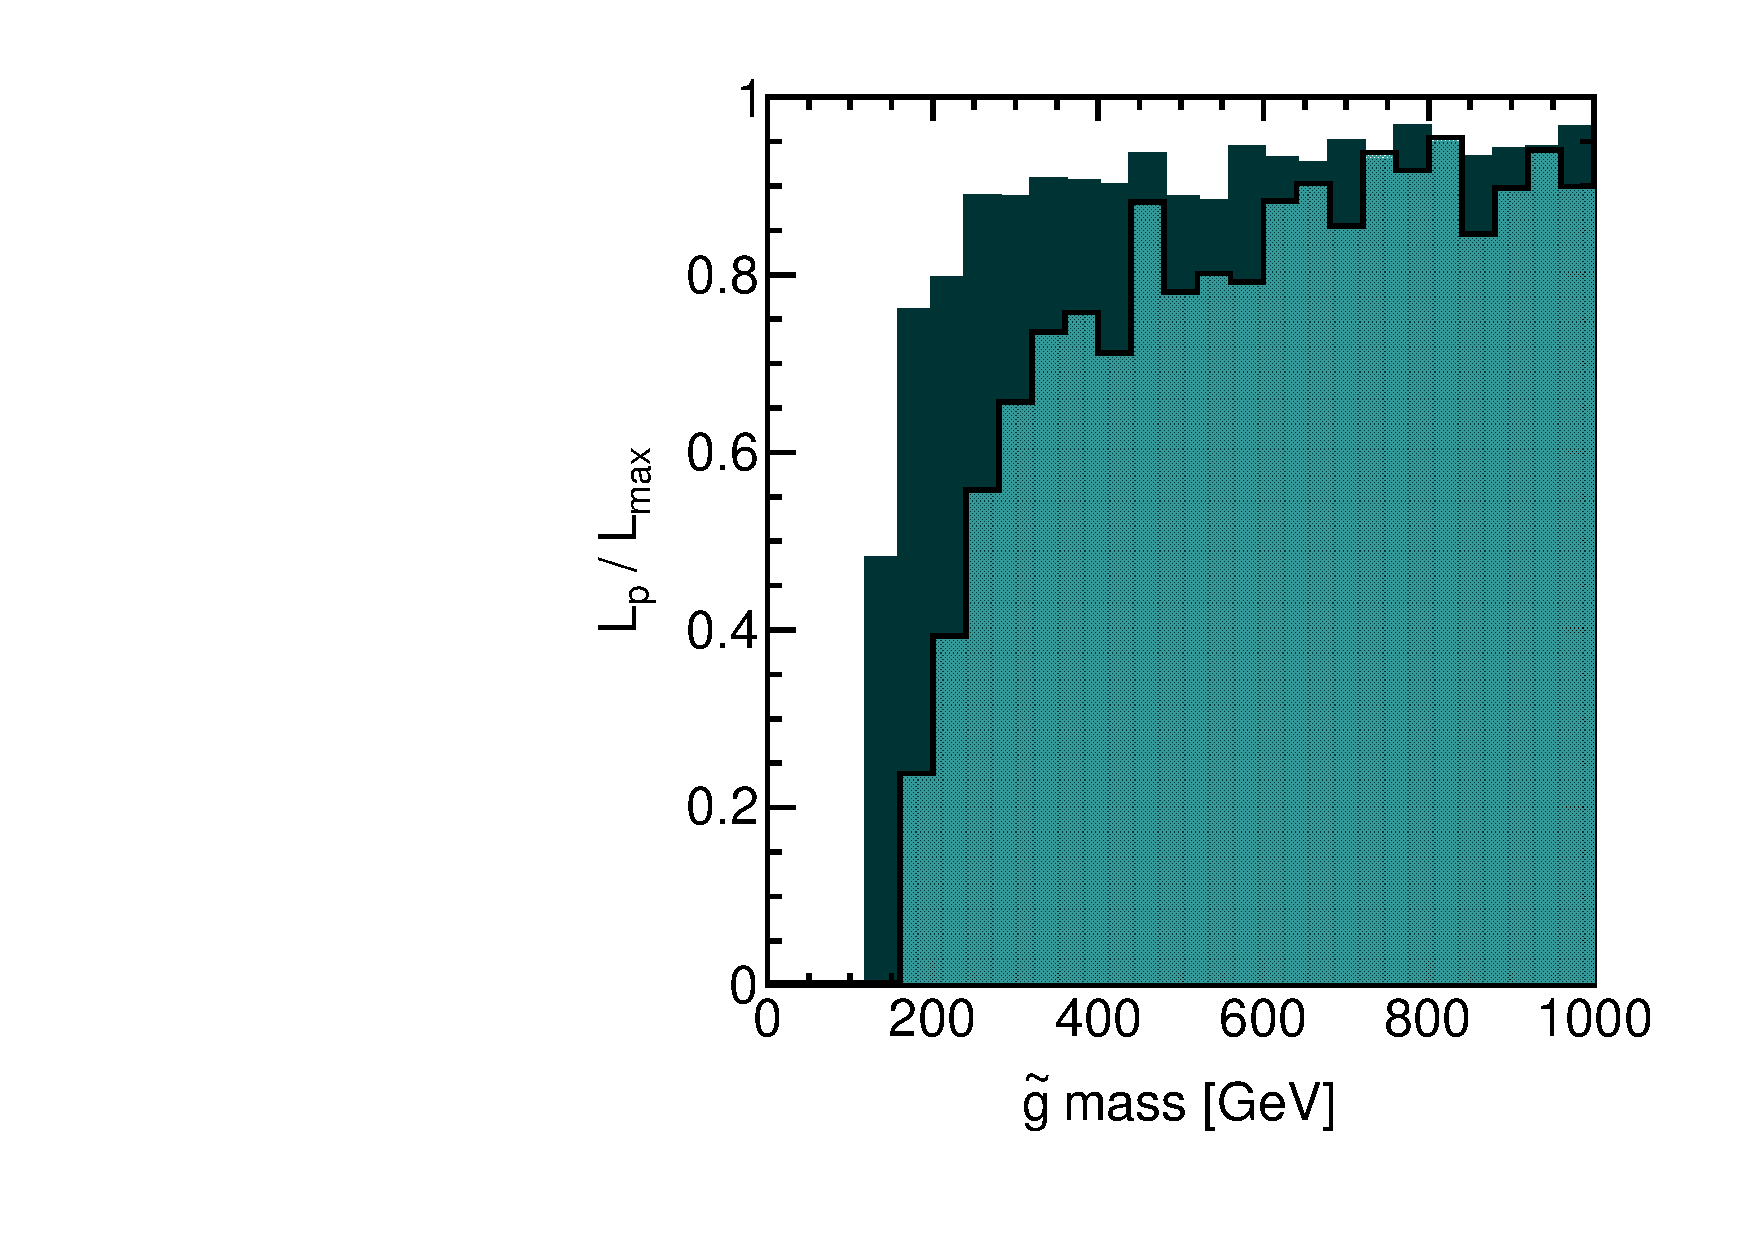
\includegraphics[height=5.5cm]{figs/fig_g.pdf} 
\caption{Ratios of profile likelihood $L_p$ to maximum likelihood $L_{max}$ shown for the gluino mass.  The colored and shaded histograms show the distributions before and after the inclusion of the CMS results.}
\label{fig:LRwcms:g}
\end{center}
\end{figure}


\begin{figure}[htbp]
\begin{center}
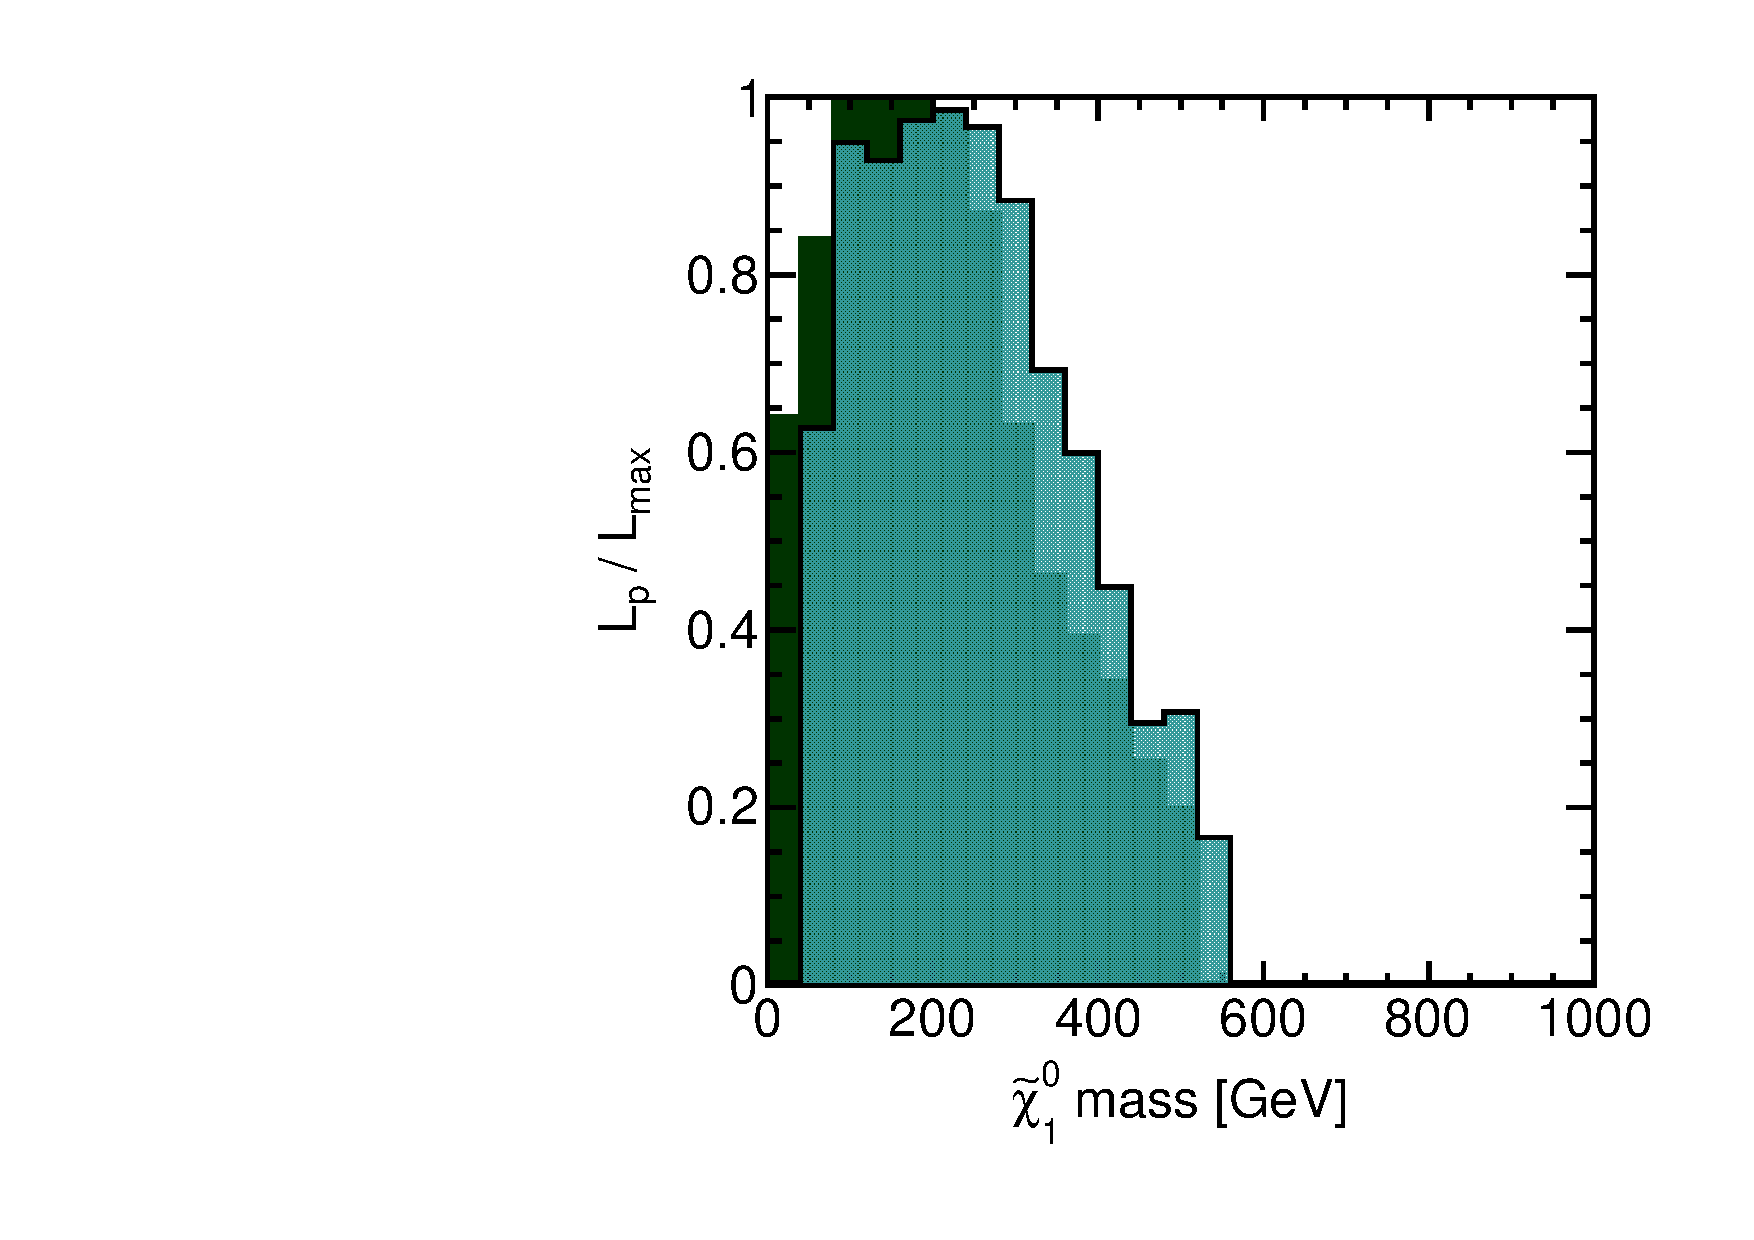
\includegraphics[height=5.5cm]{figs/fig_chi_1_0.pdf} 
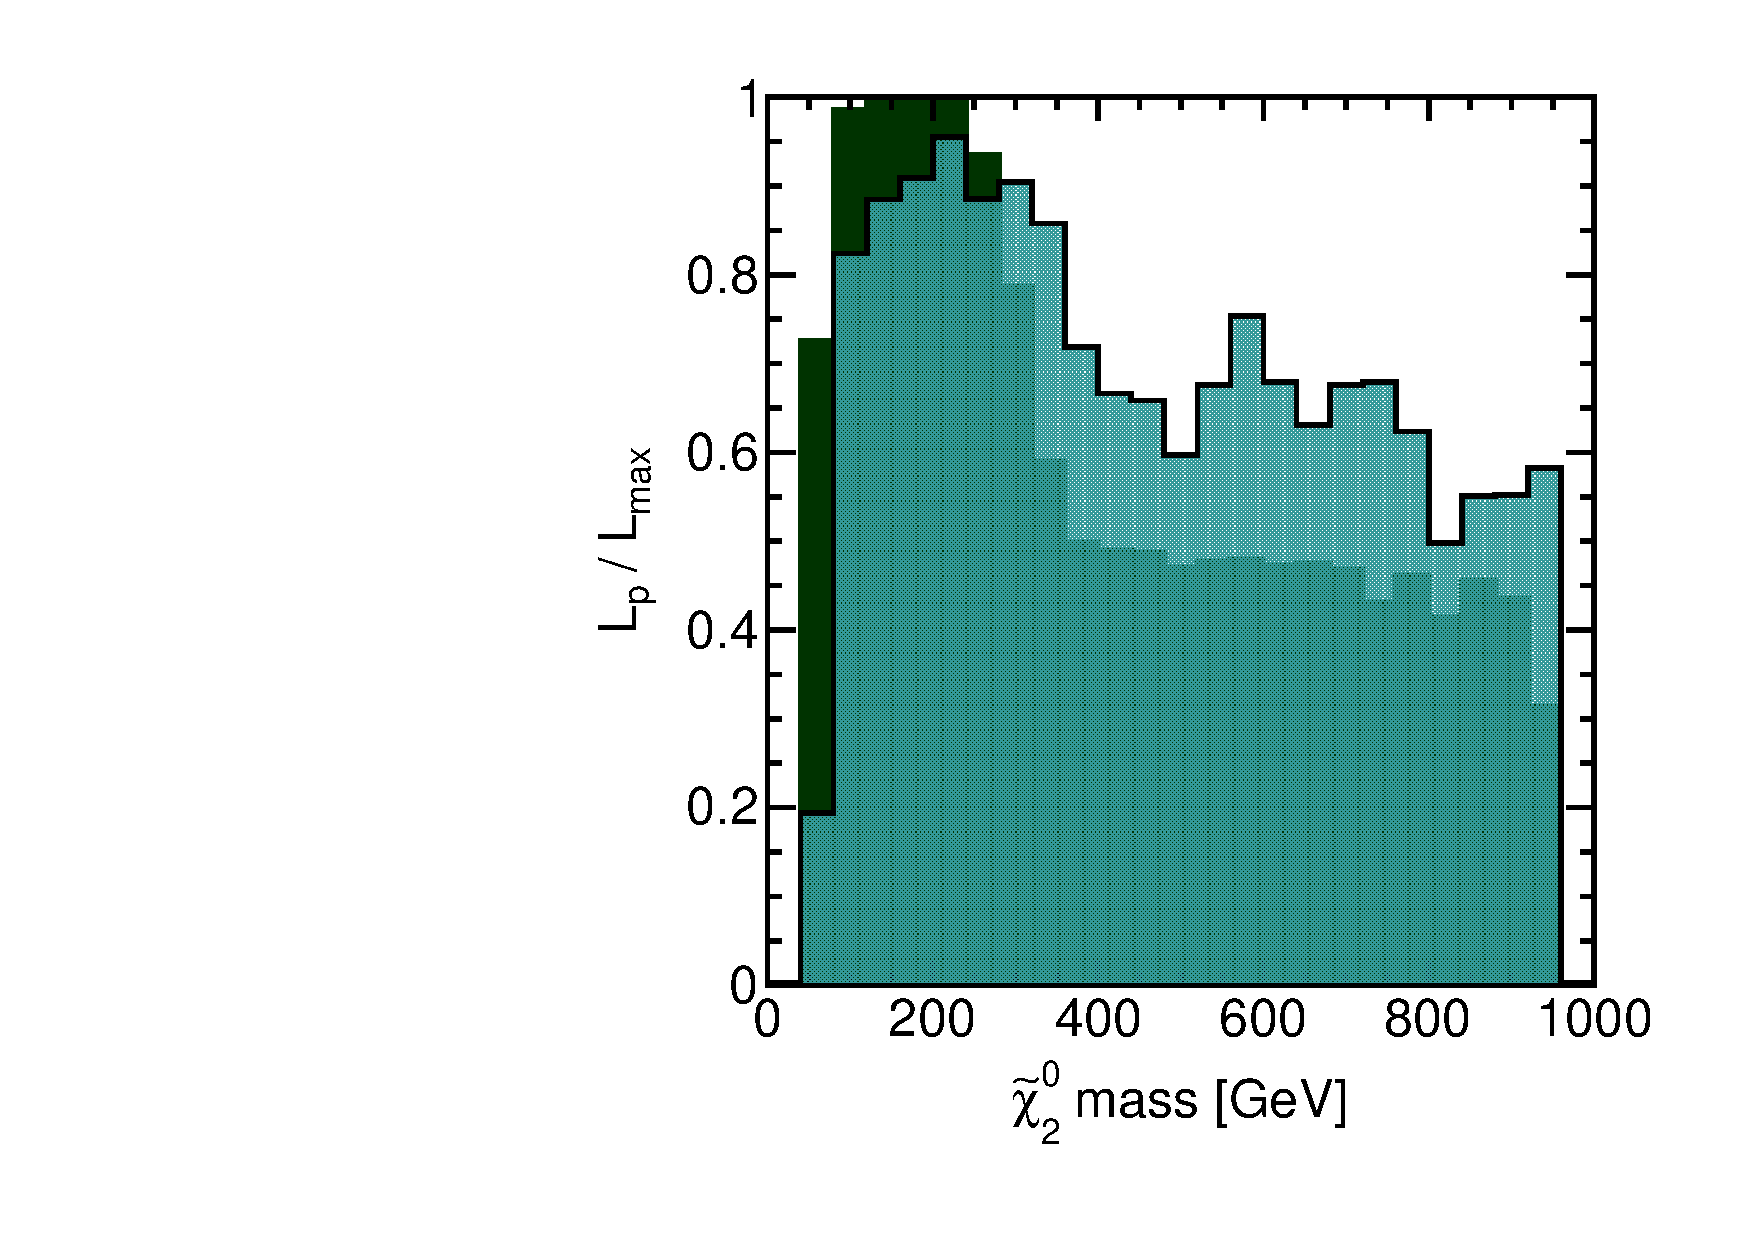
\includegraphics[height=5.5cm]{figs/fig_chi_2_0.pdf} \\
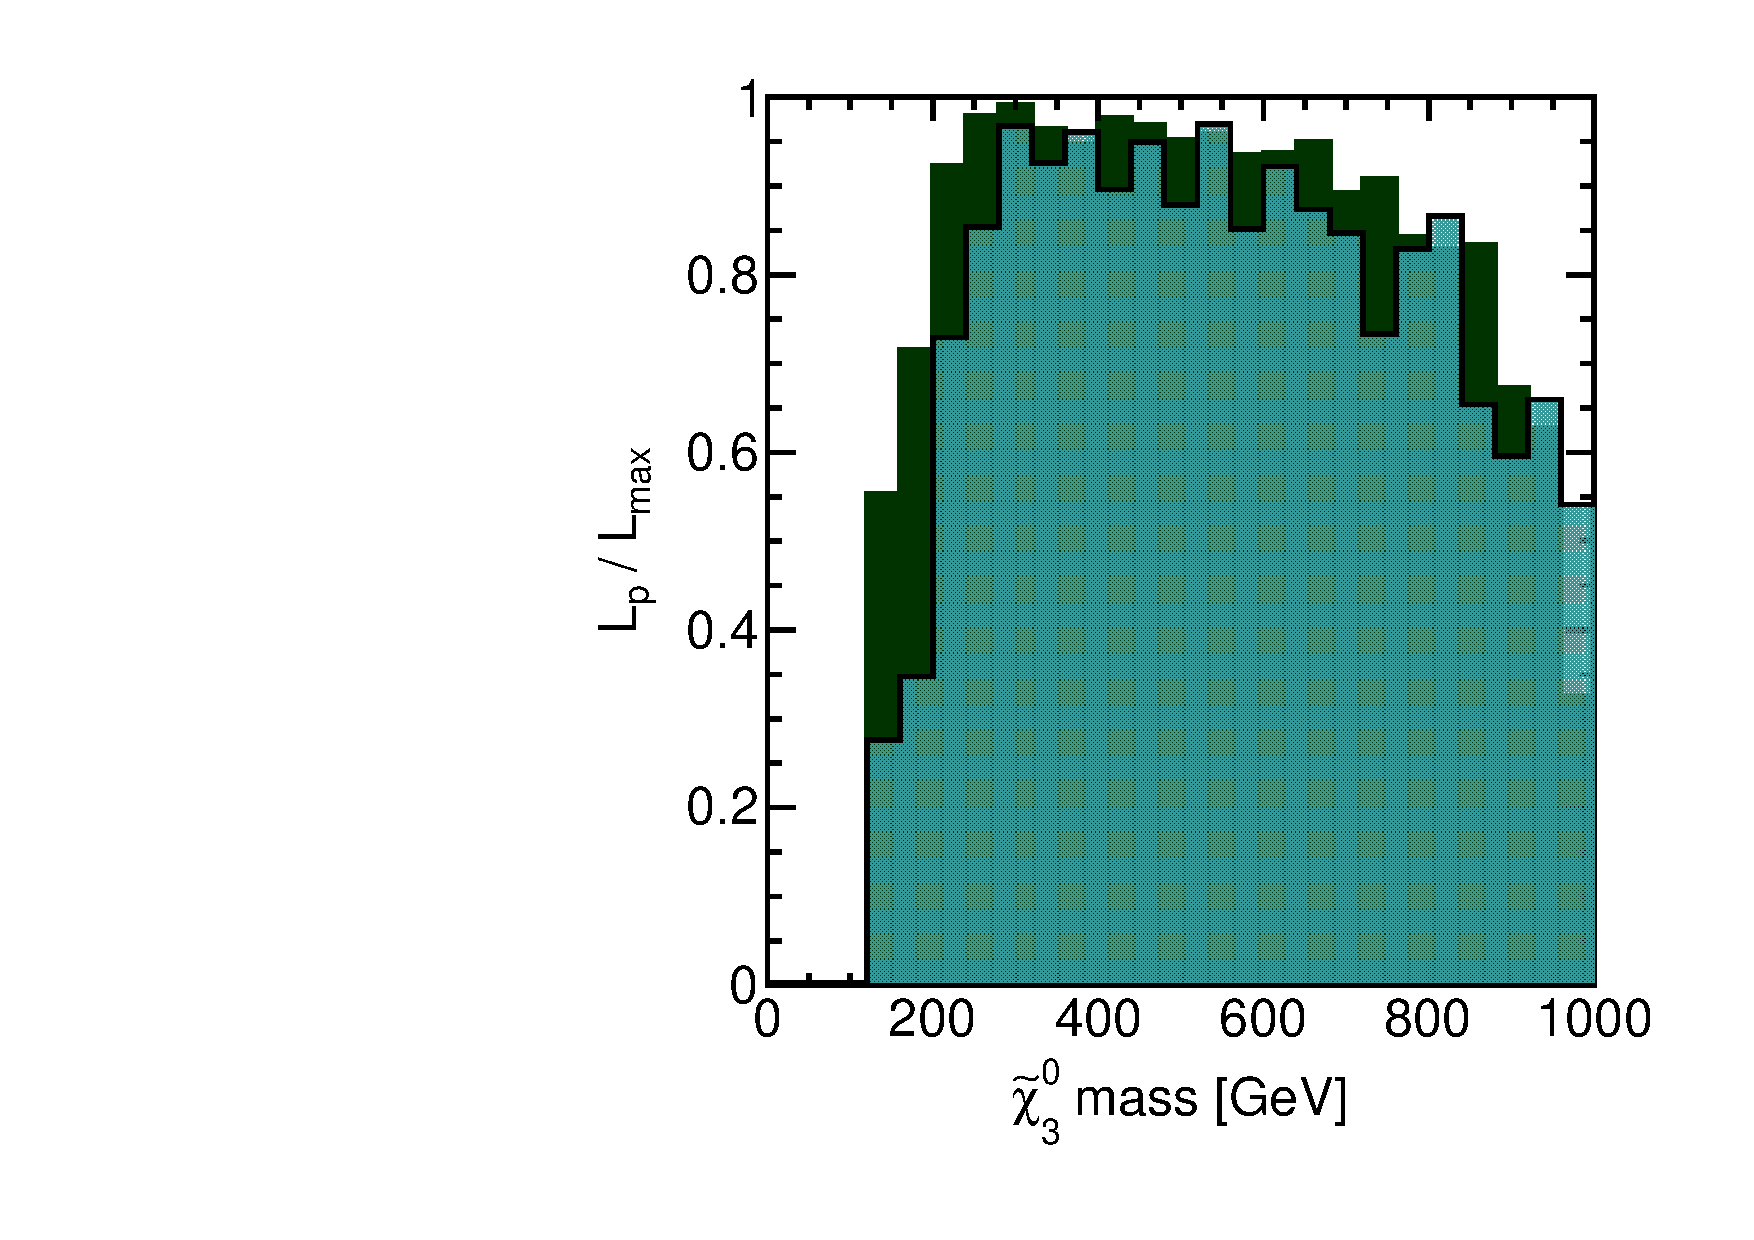
\includegraphics[height=5.5cm]{figs/fig_chi_3_0.pdf} 
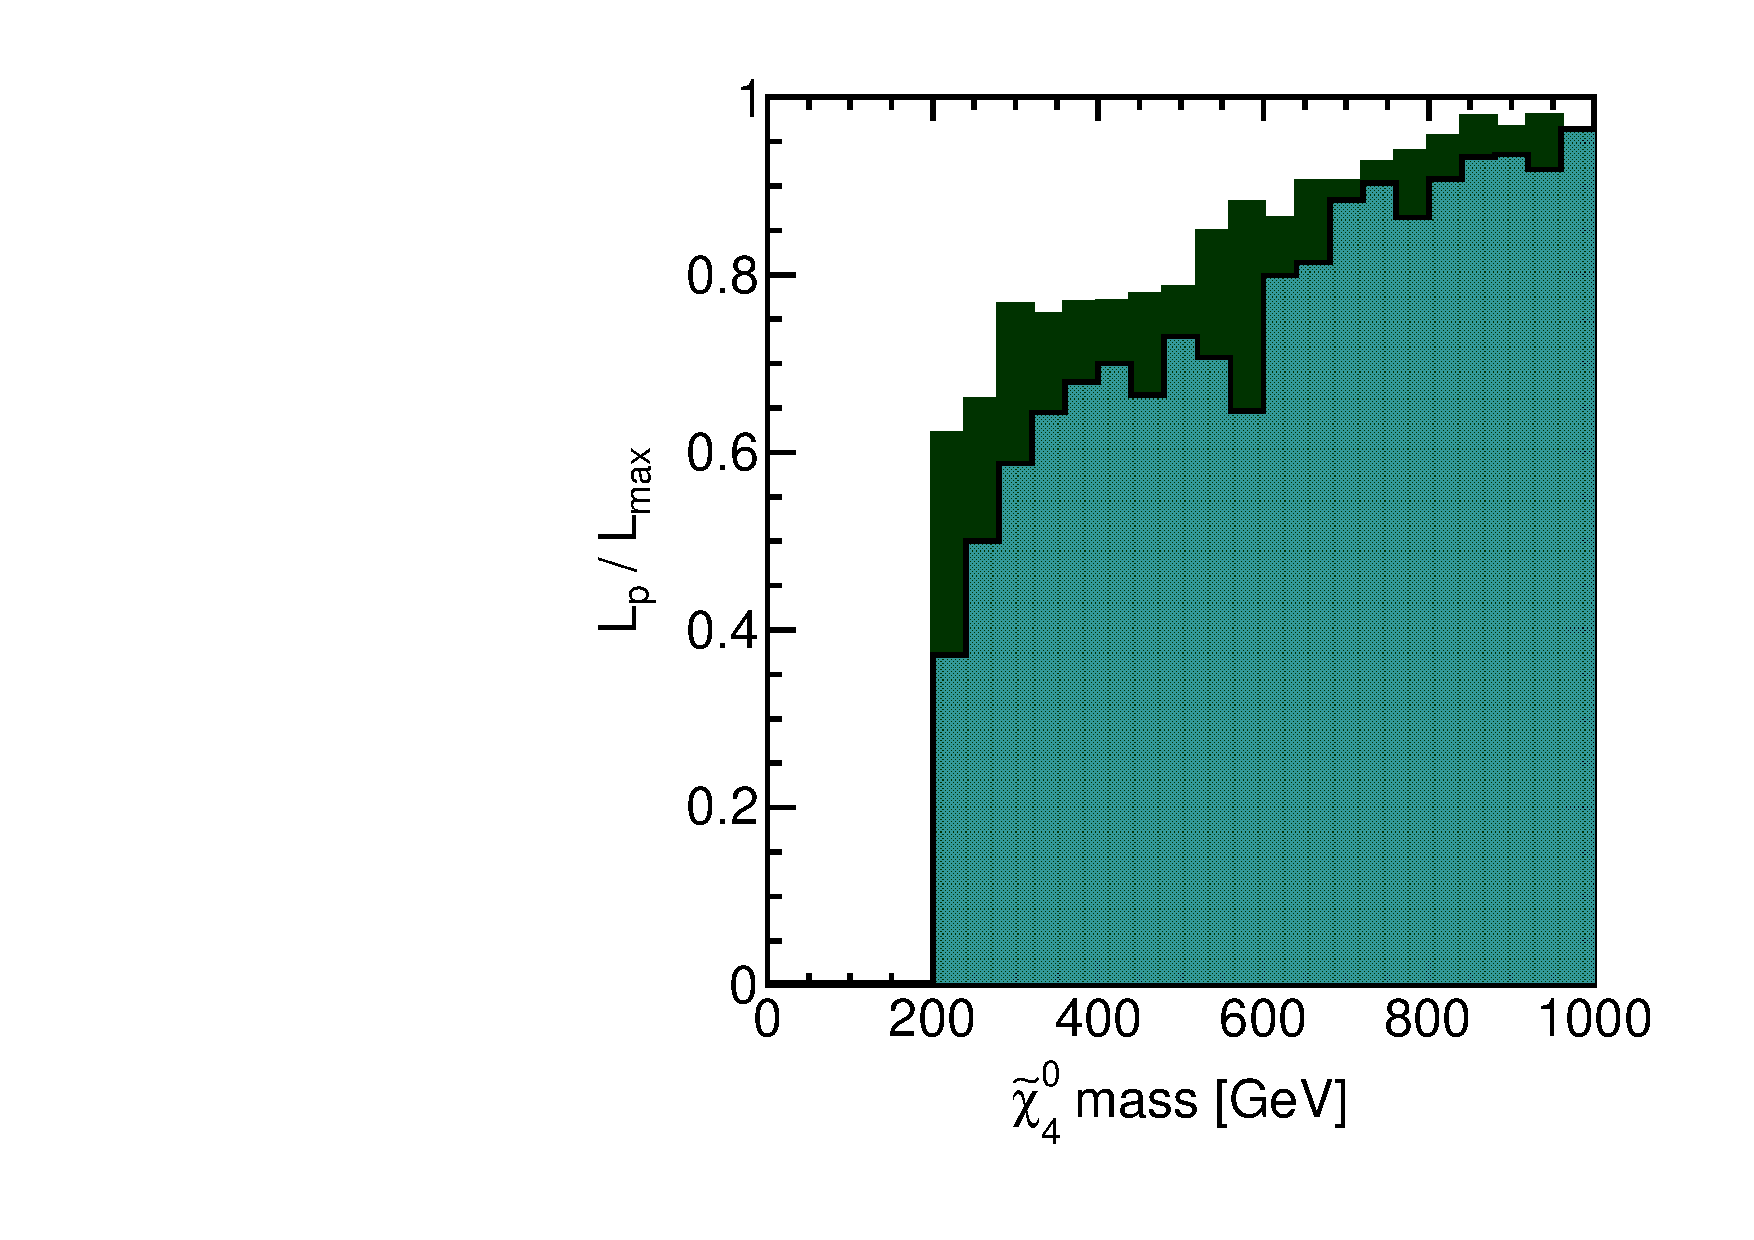
\includegraphics[height=5.5cm]{figs/fig_chi_4_0.pdf} 
\caption{Ratios of profile likelihood $L_p$ to maximum likelihood $L_{max}$ shown for the neutralino masses.  The colored and shaded histograms show the distributions before and after the inclusion of the CMS results.}
\label{fig:LRwcms_chi0}
\end{center}
\end{figure}

\begin{figure}[htbp]
\begin{center}
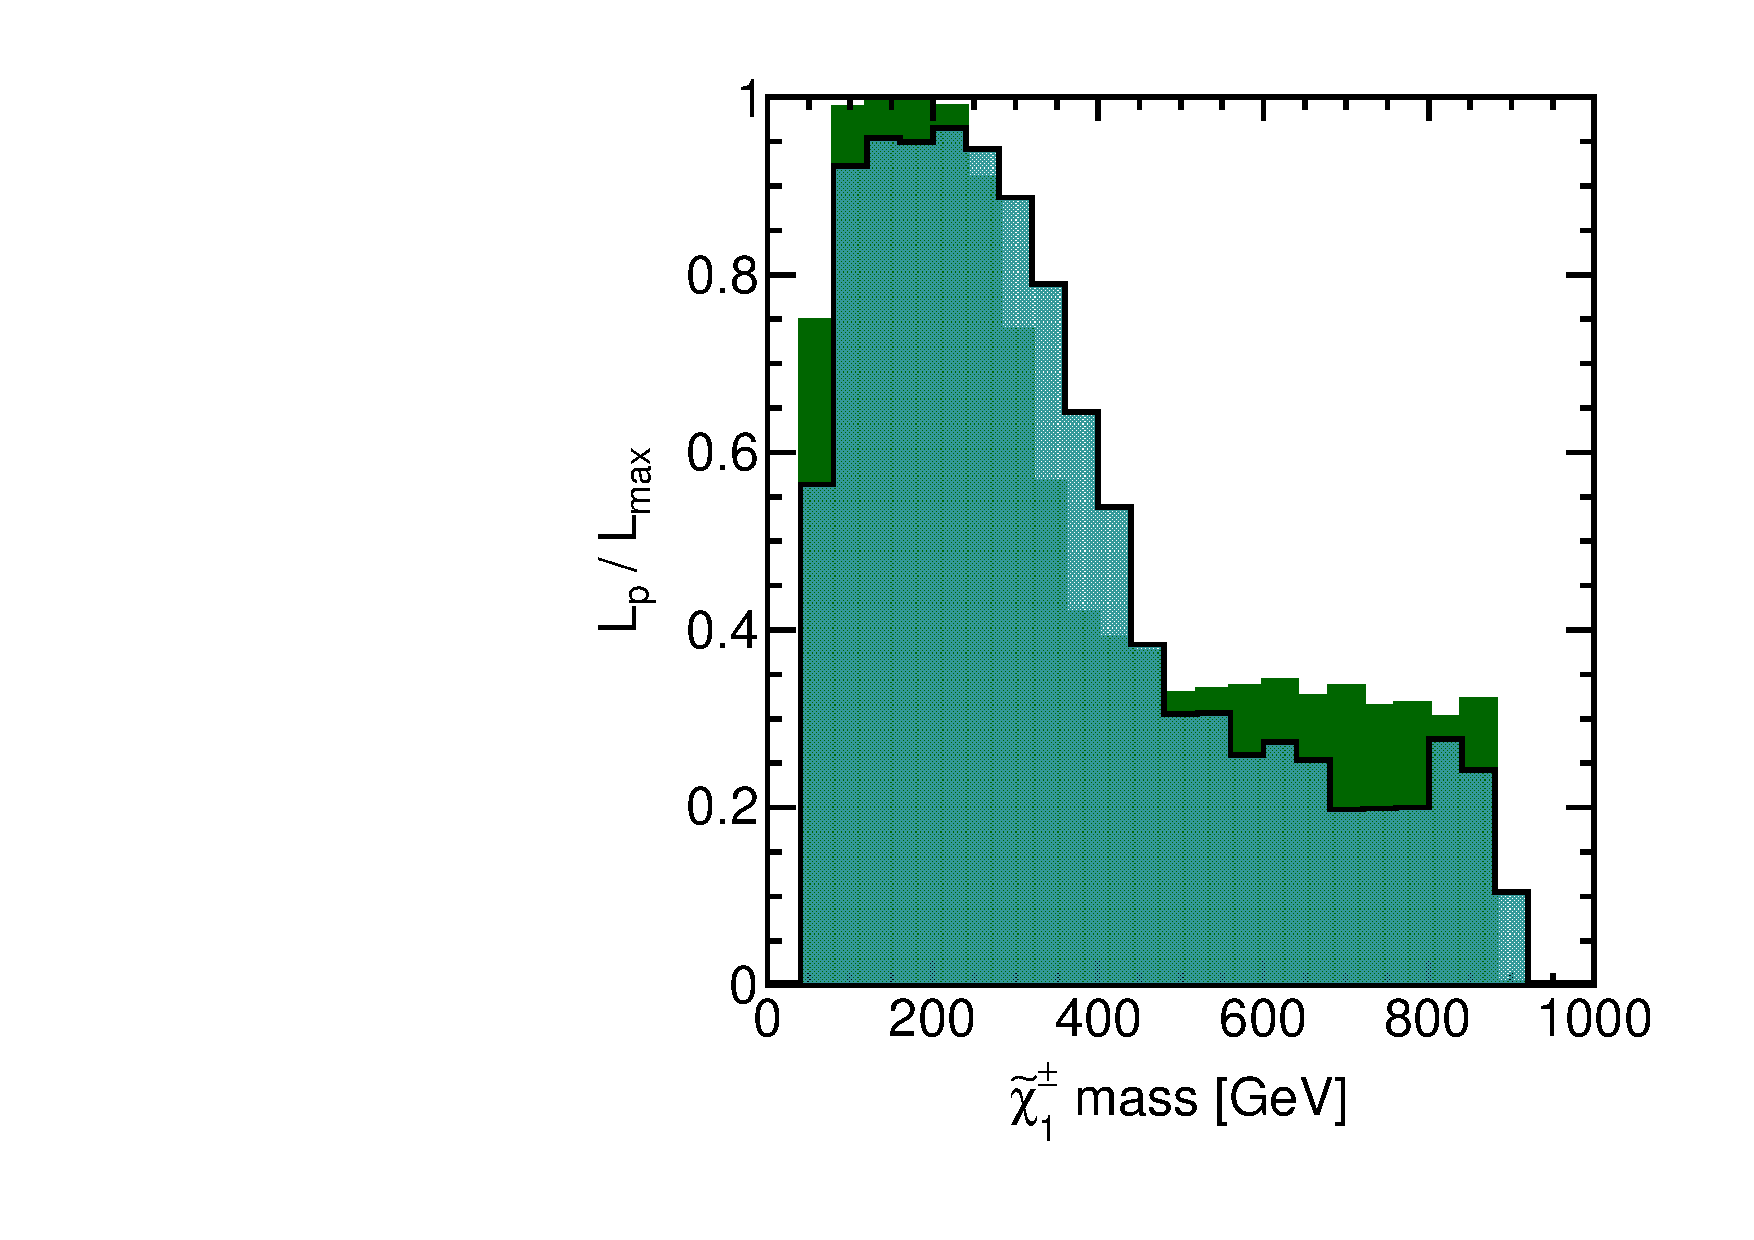
\includegraphics[height=5.5cm]{figs/fig_chi_1_pm.pdf} 
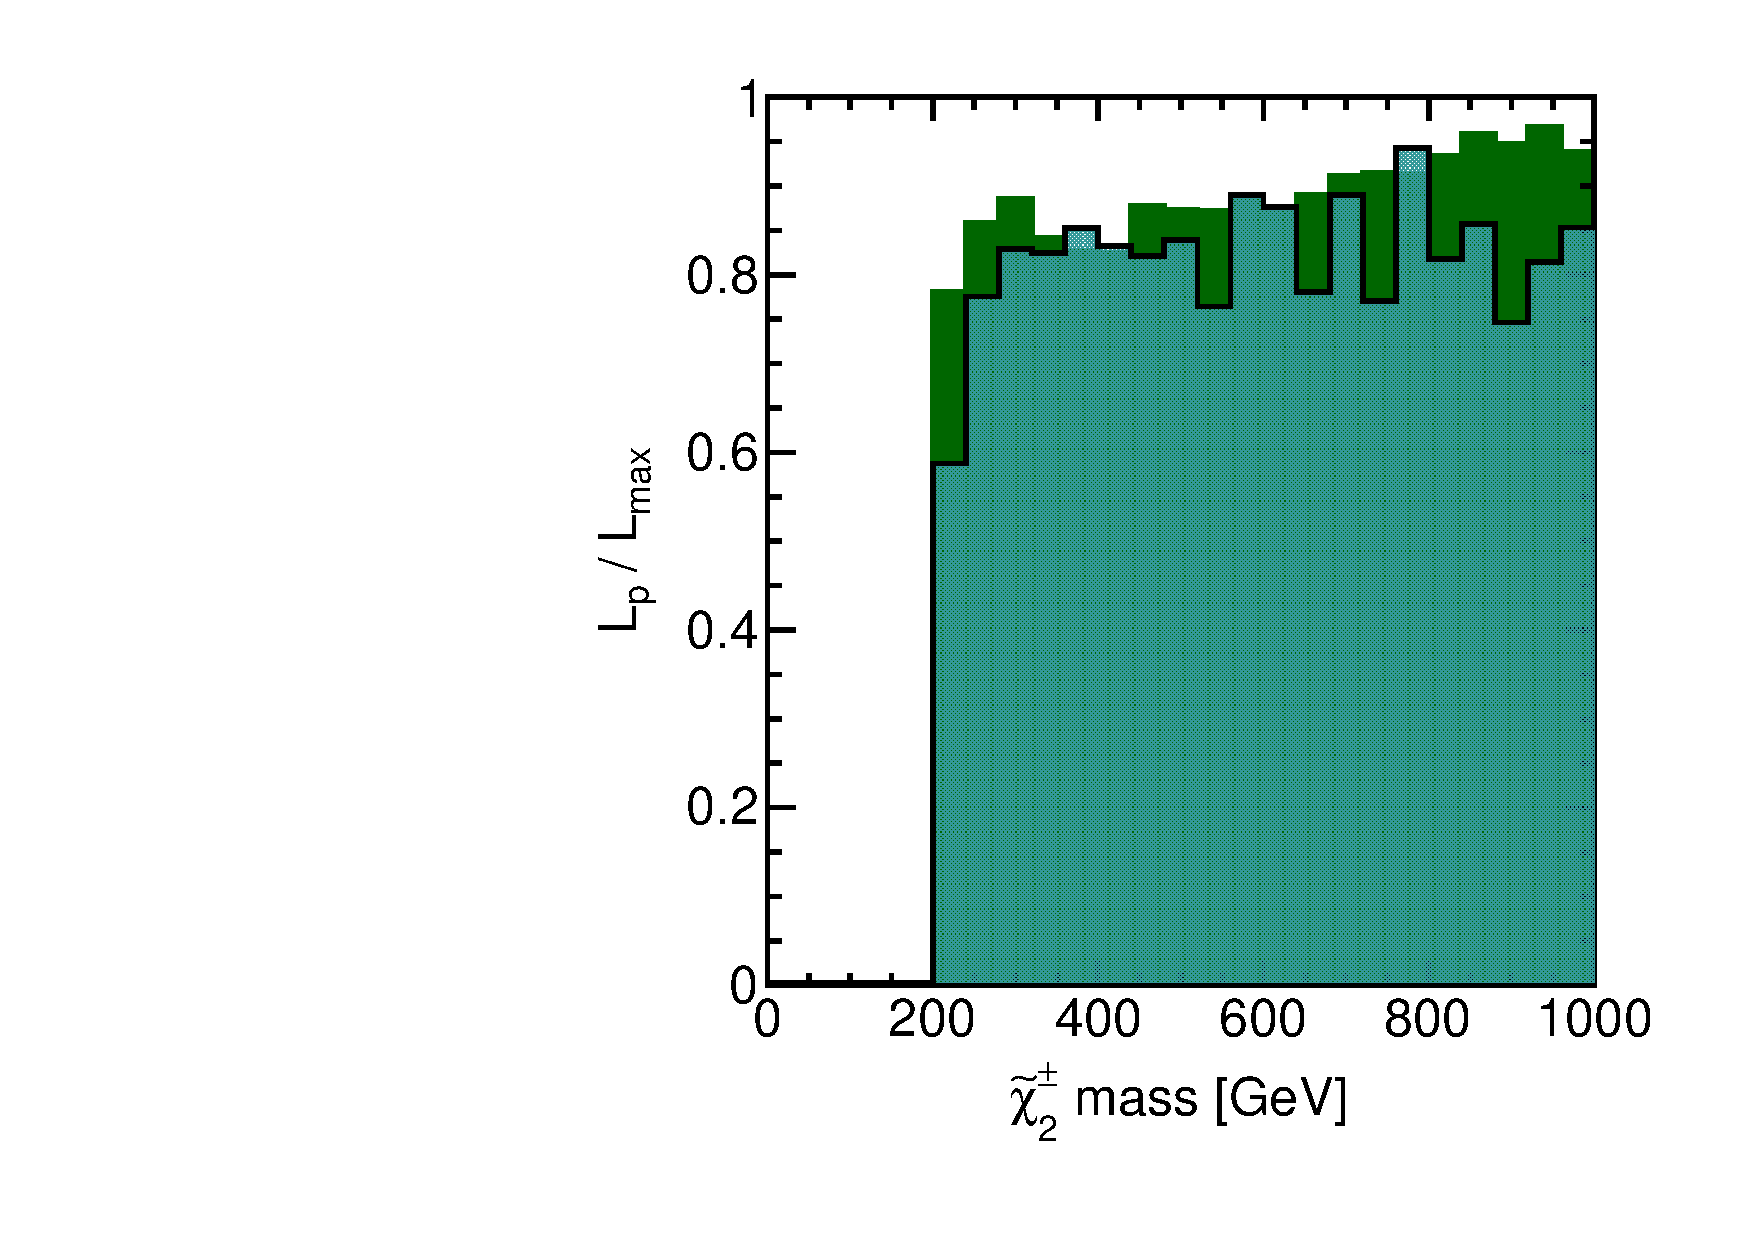
\includegraphics[height=5.5cm]{figs/fig_chi_2_pm.pdf}
\caption{Ratios of profile likelihood $L_p$ to maximum likelihood $L_{max}$ shown for chargino masses.  The colored and shaded histograms show the distributions before and after the inclusion of the CMS results.}
\label{fig:LRwcms_chipm}
\end{center}
\end{figure}


\begin{figure}[htbp]
\begin{center}
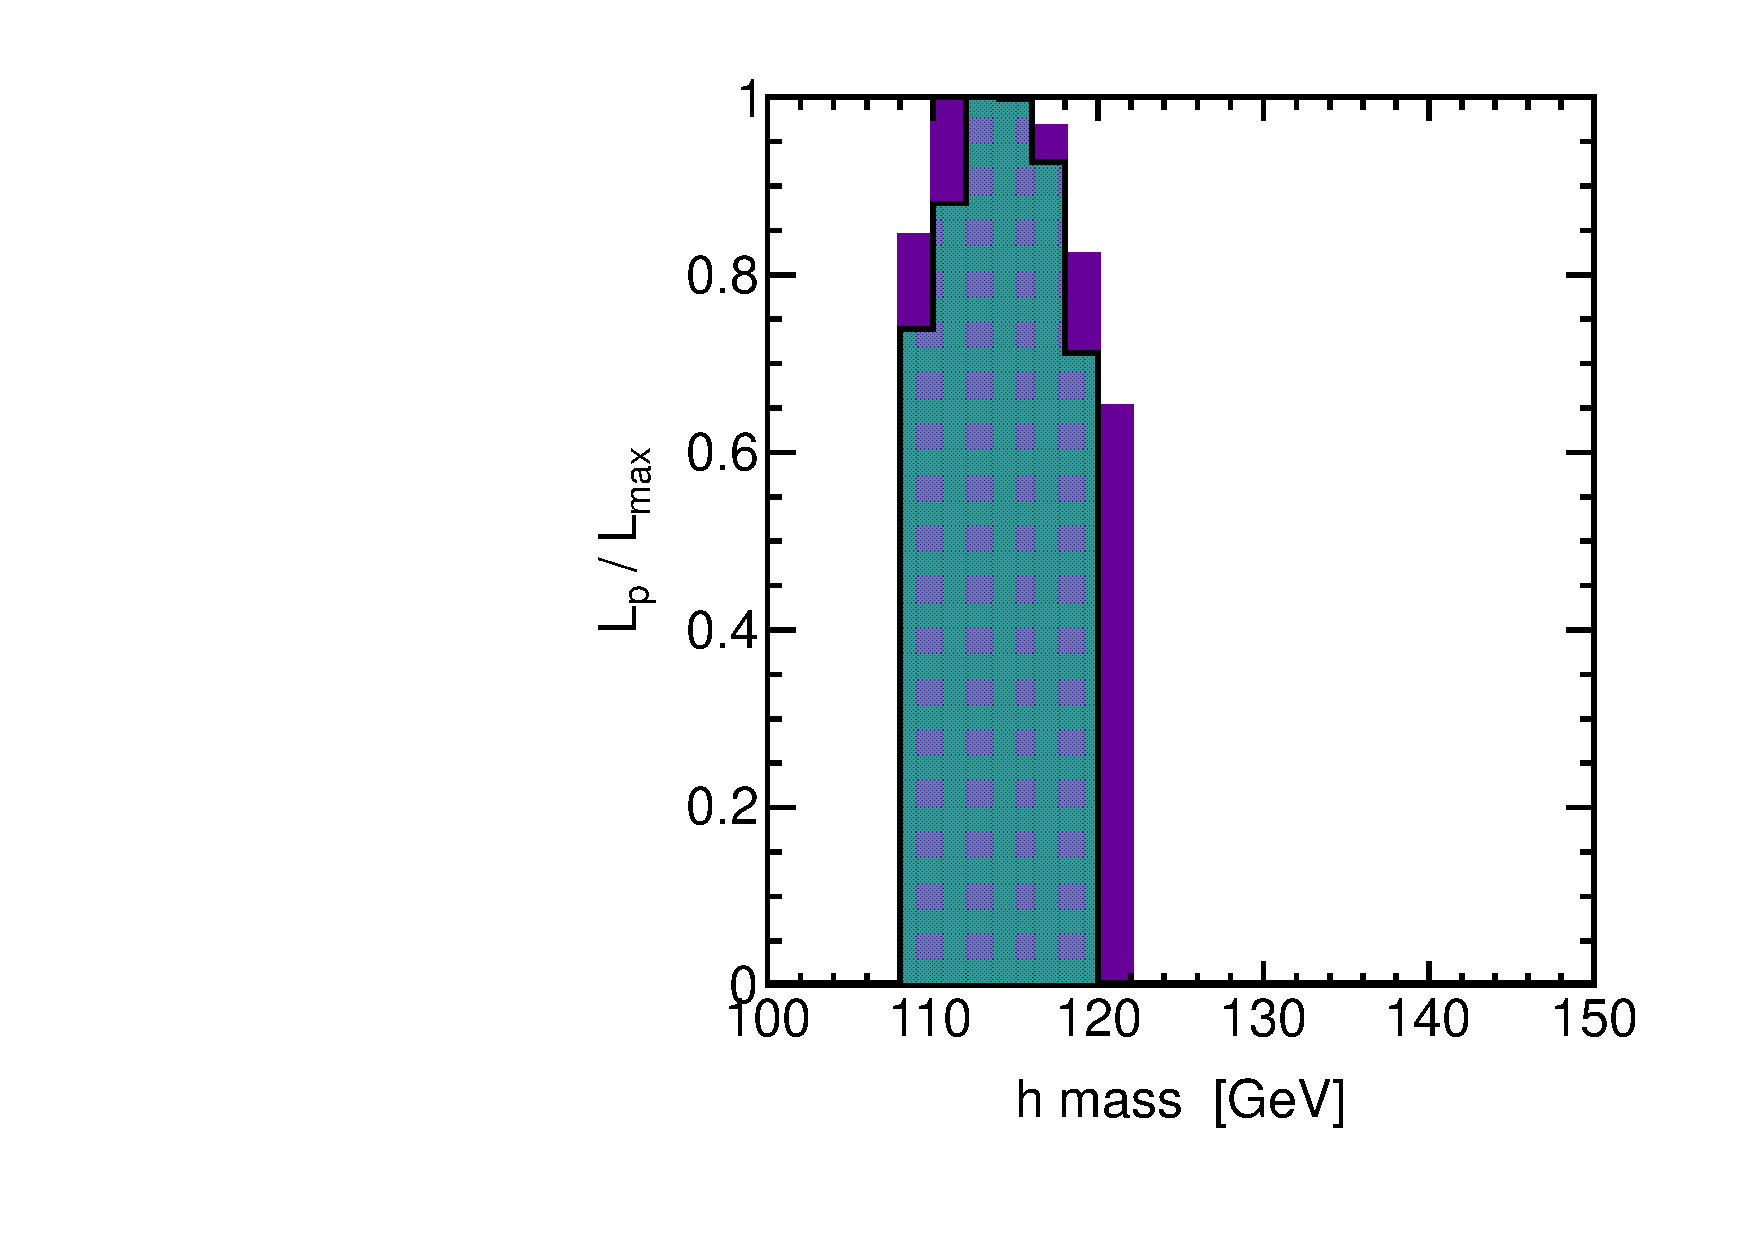
\includegraphics[height=5.5cm]{figs/fig_h.pdf} 
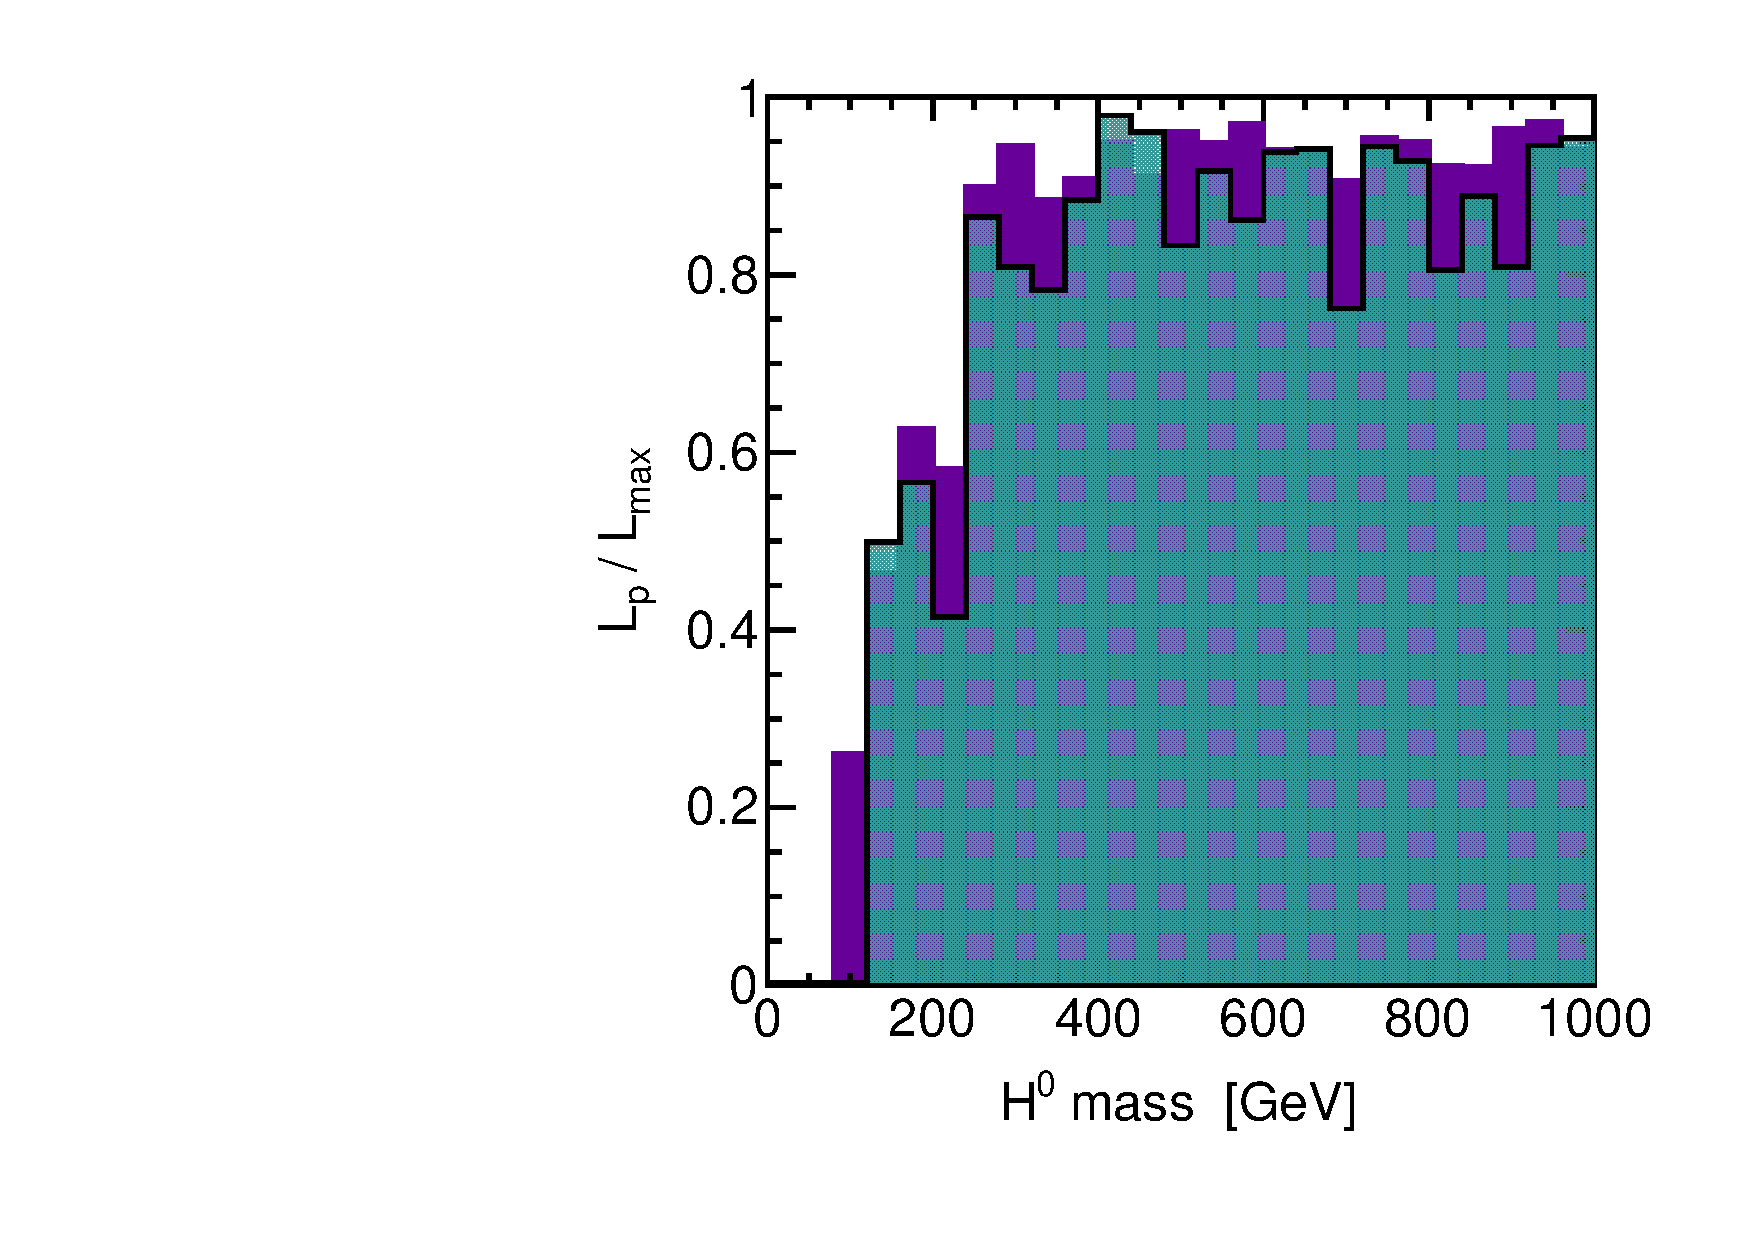
\includegraphics[height=5.5cm]{figs/fig_H0.pdf} \\
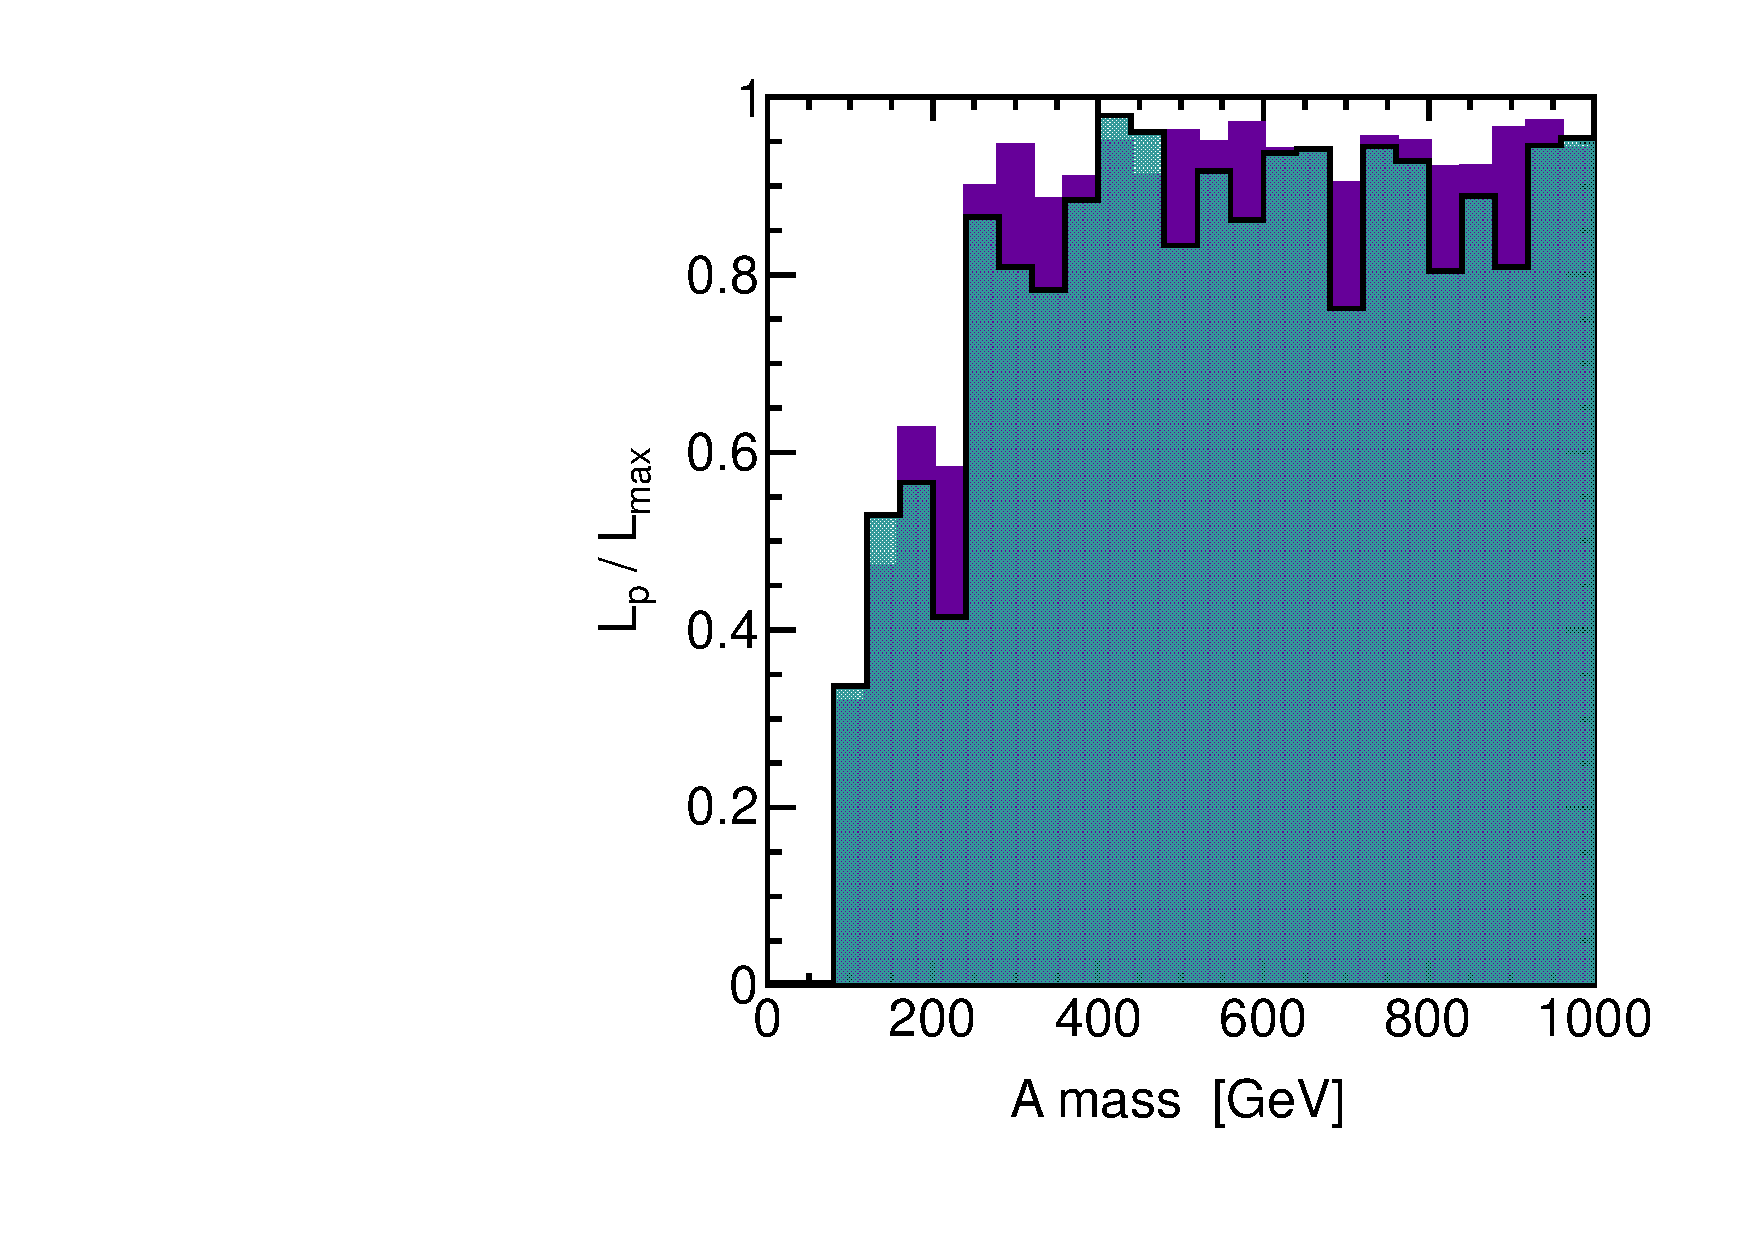
\includegraphics[height=5.5cm]{figs/fig_A.pdf} 
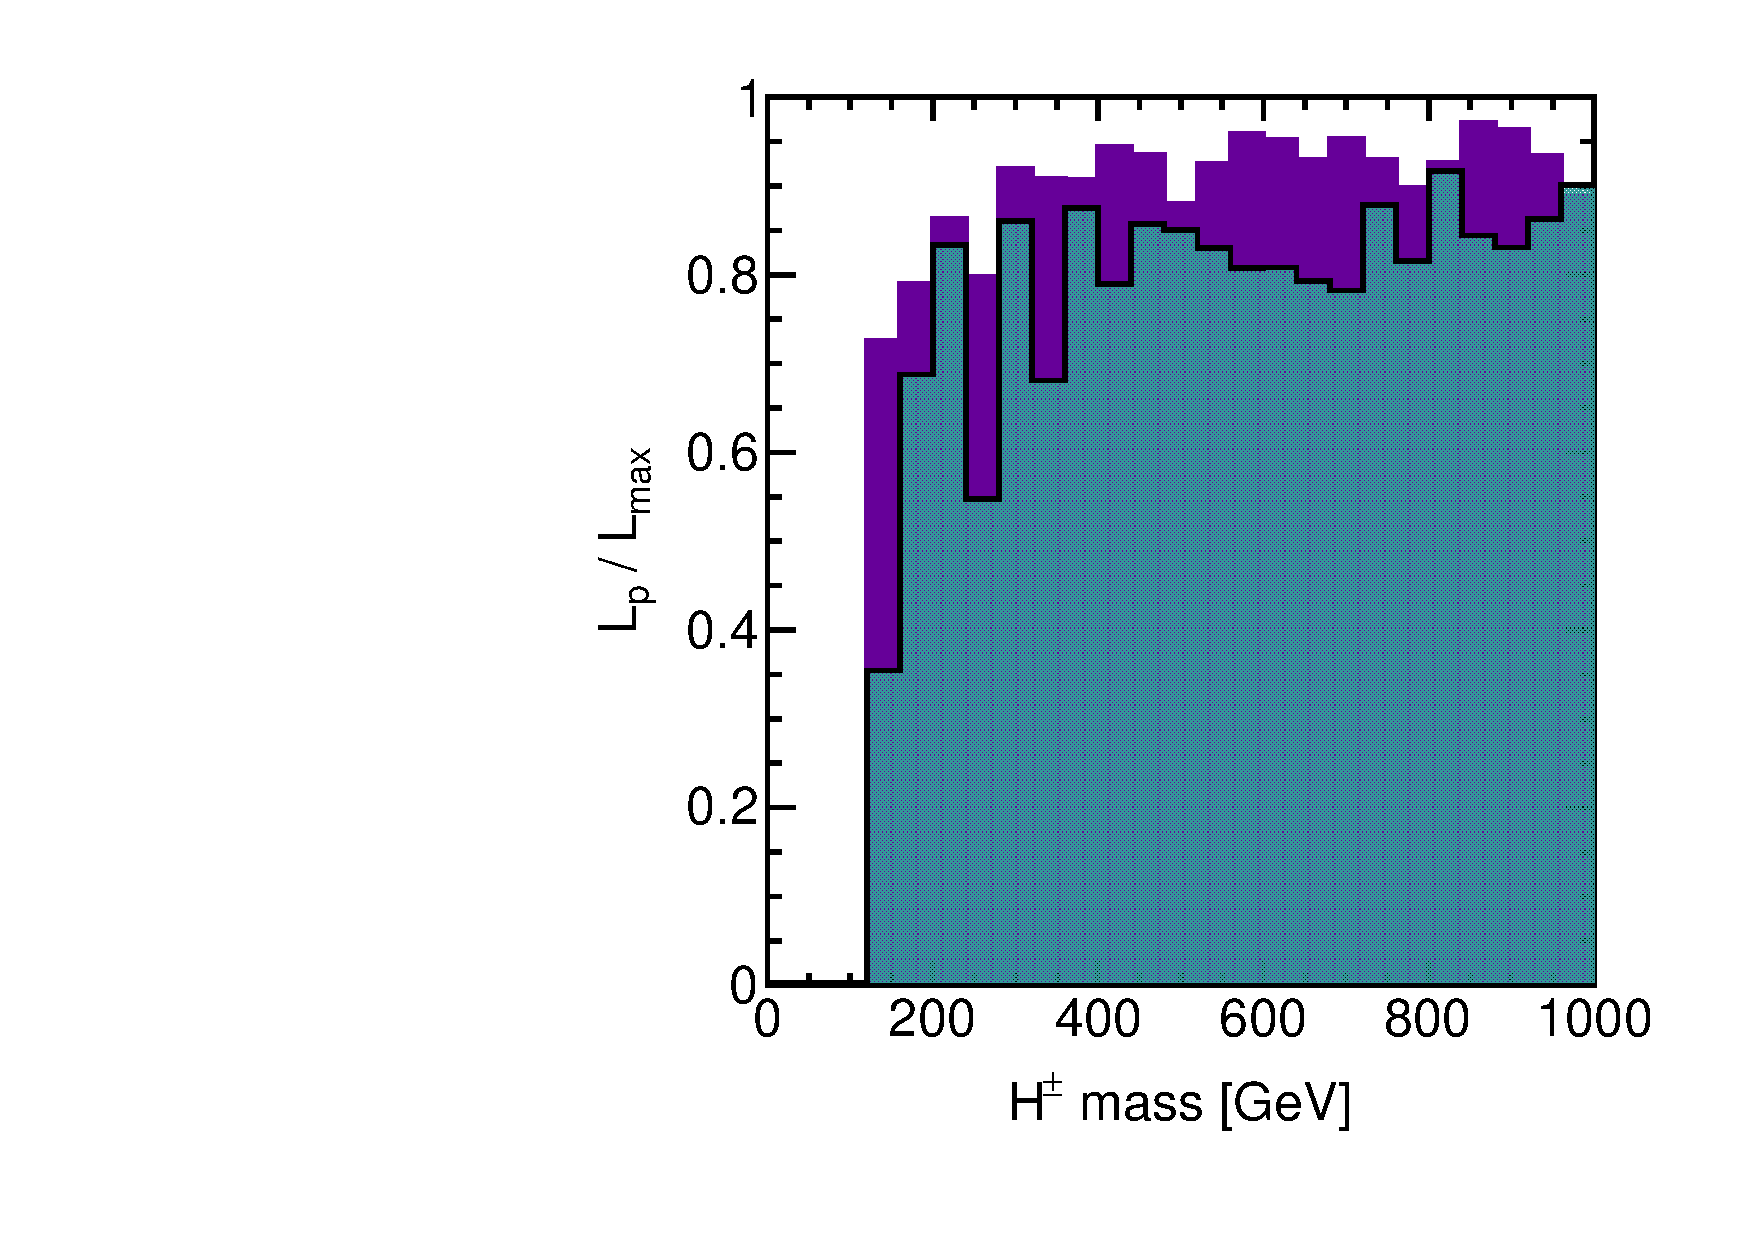
\includegraphics[height=5.5cm]{figs/fig_H_pm.pdf} 
\caption{Ratios of profile likelihood $L_p$ to maximum likelihood $L_{max}$ shown for the Higgs masses.  The colored and shaded histograms show the distributions before and after the inclusion of the CMS results.}
\label{fig:LRwcms_Higgs}
\end{center}
\end{figure}


\begin{figure}[htbp]
\begin{center}
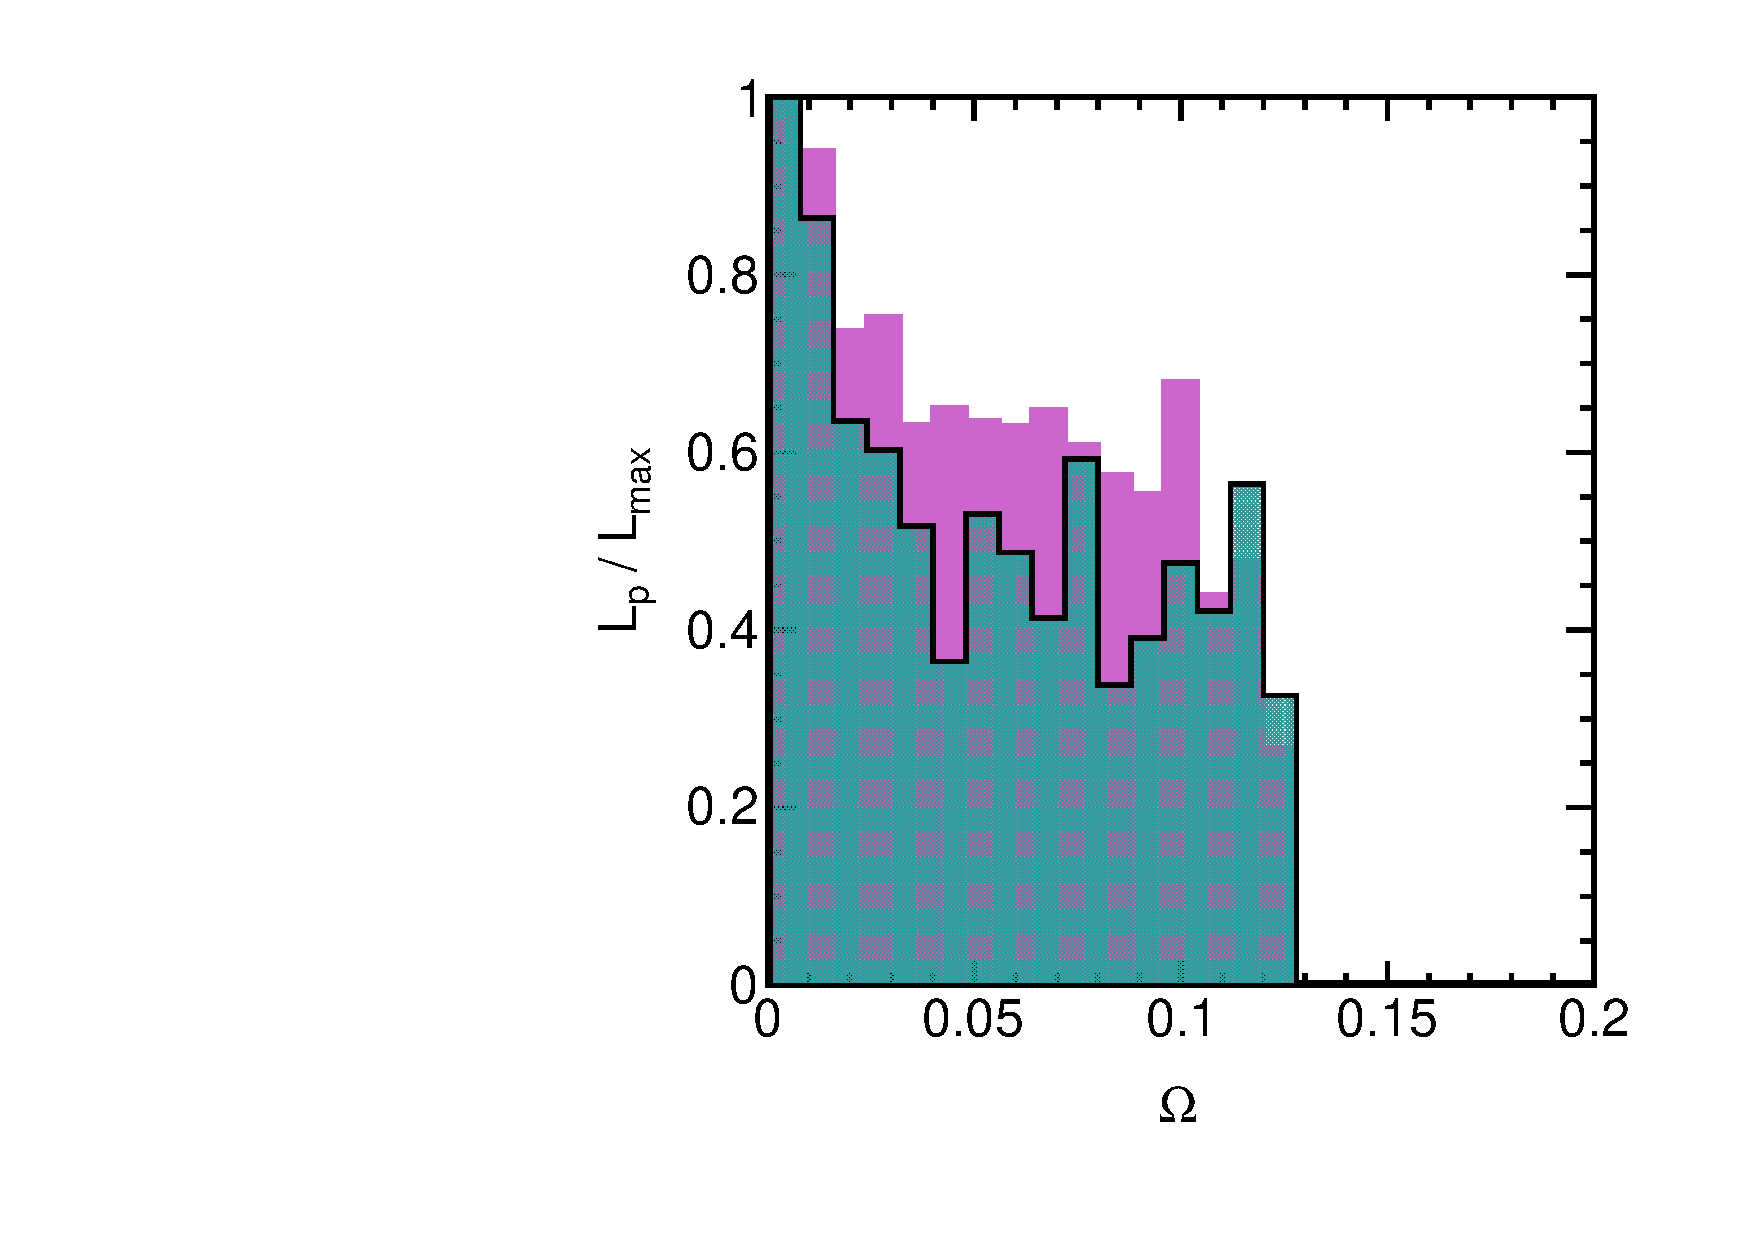
\includegraphics[height=5.5cm]{figs/fig_omega_m.pdf} 
\caption{Ratio of profile likelihood $L_p$ to maximum likelihood $L_{max}$ shown for lightest neutralino dark matter relic density.  The colored and shaded histograms show the distributions before and after the inclusion of the CMS results.}
\label{fig:LRwcms_omg}
\end{center}
\end{figure}


%\begin{figure}[htbp]
%\begin{center}
%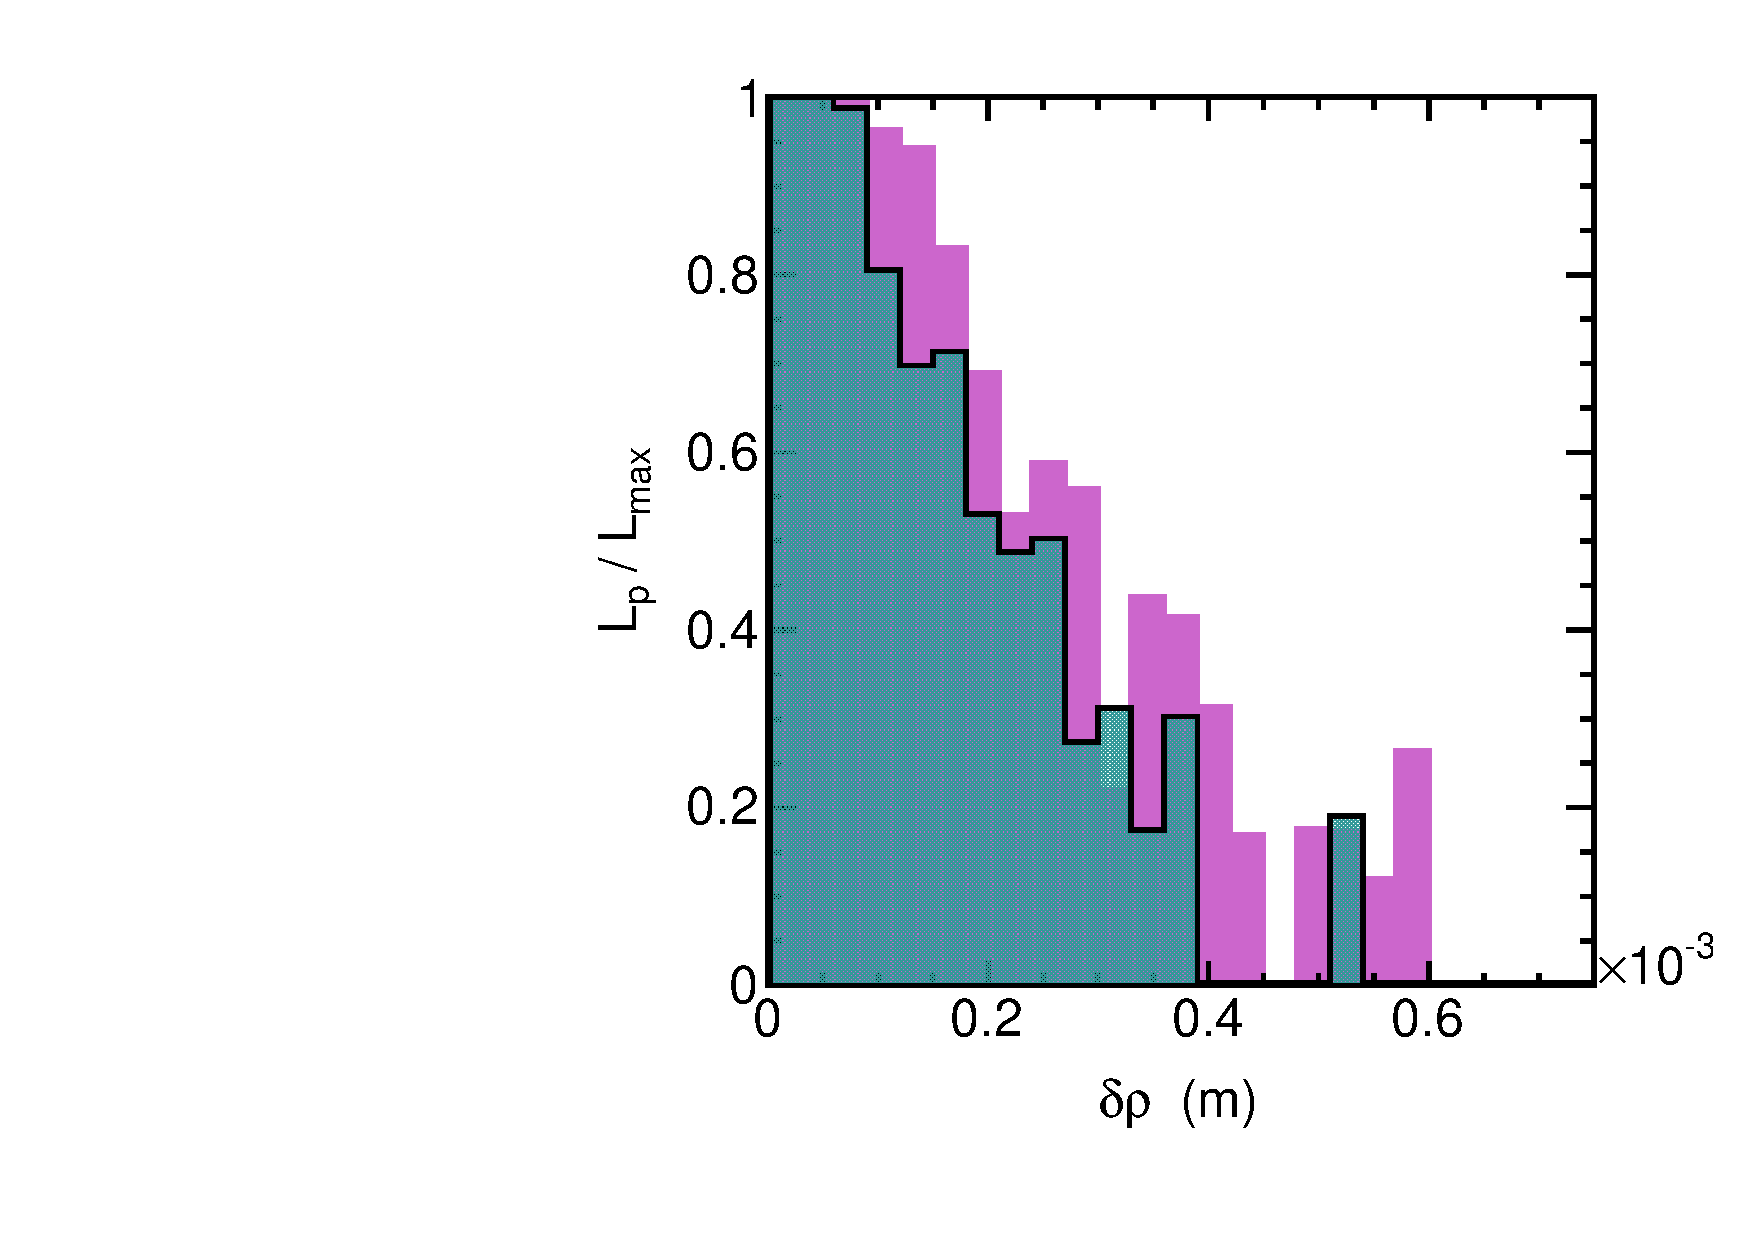
\includegraphics[height=5.5cm]{figs/fig_drho_m.pdf} 
%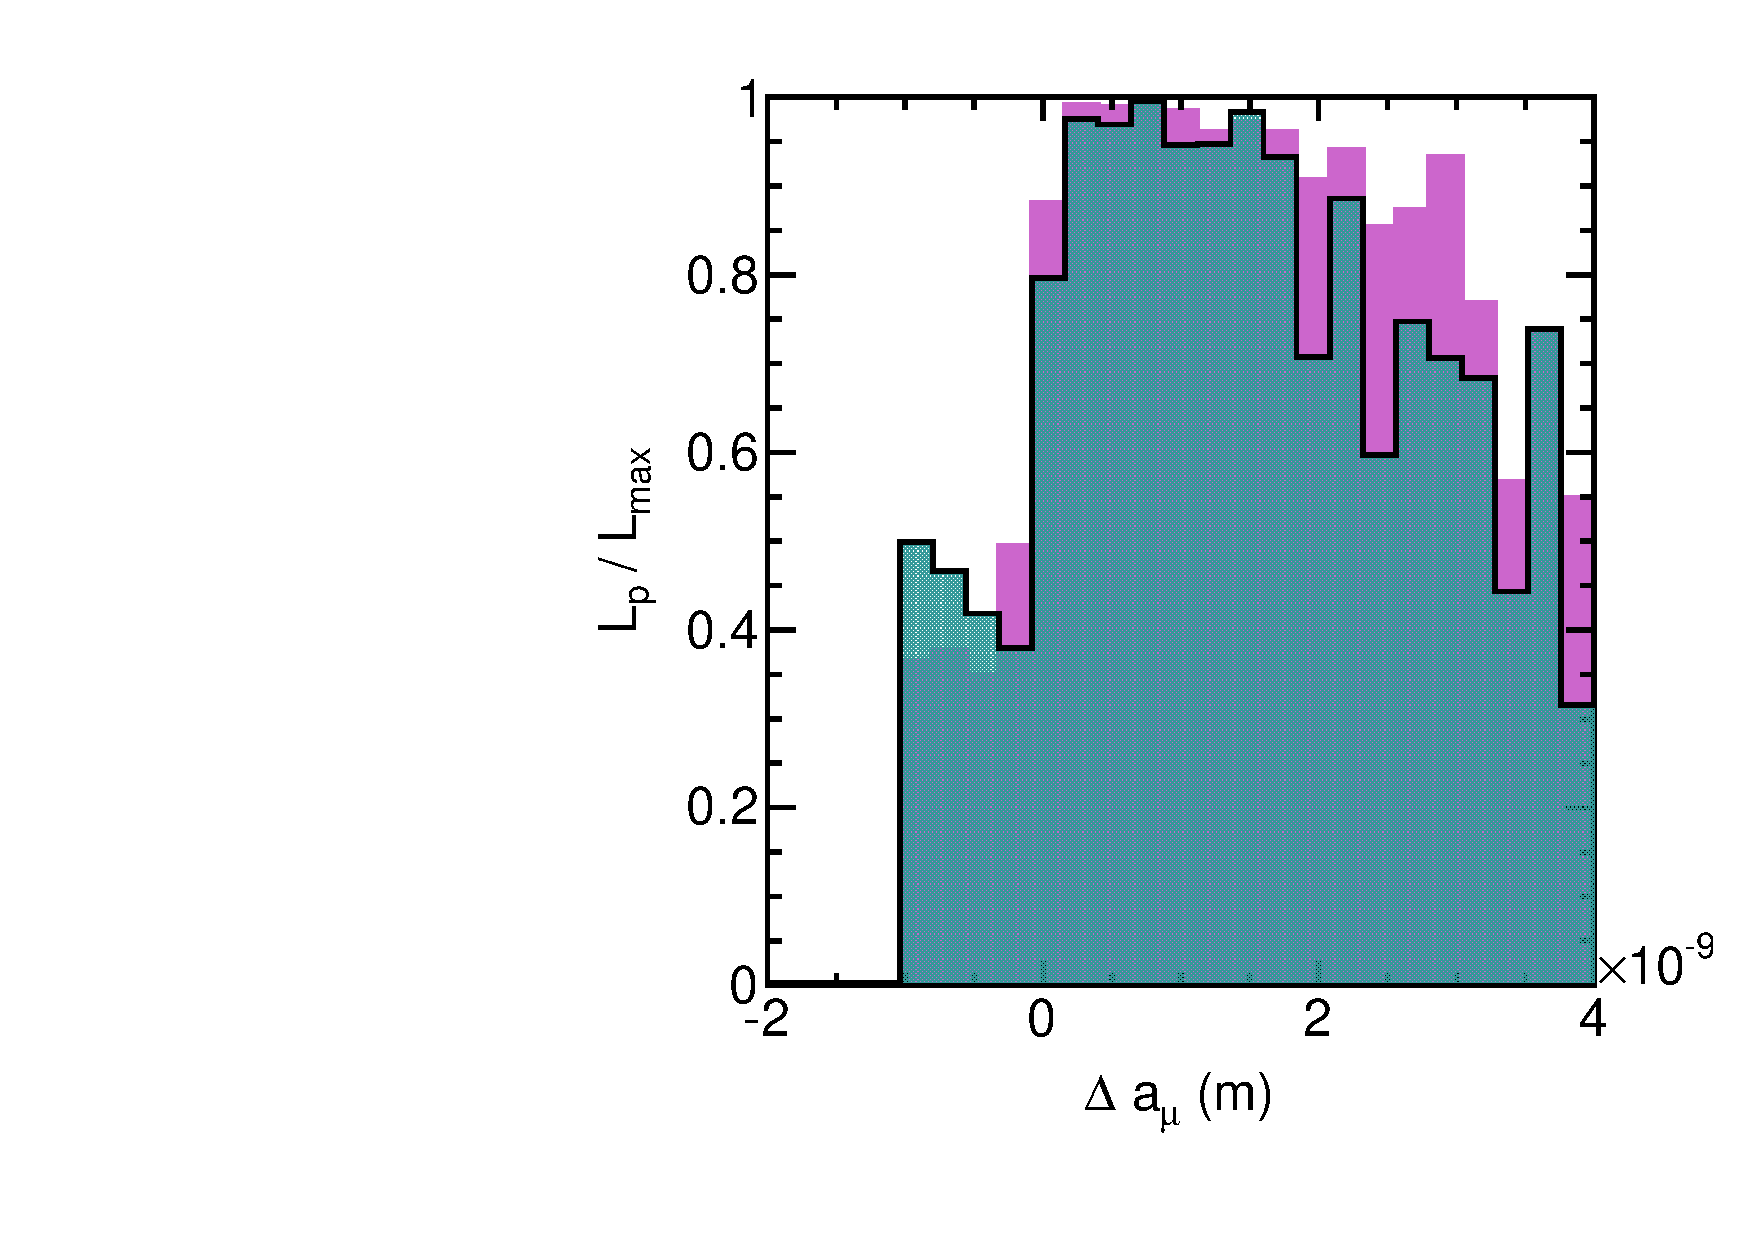
\includegraphics[height=5.5cm]{figs/fig_gmu_m.pdf} \\
%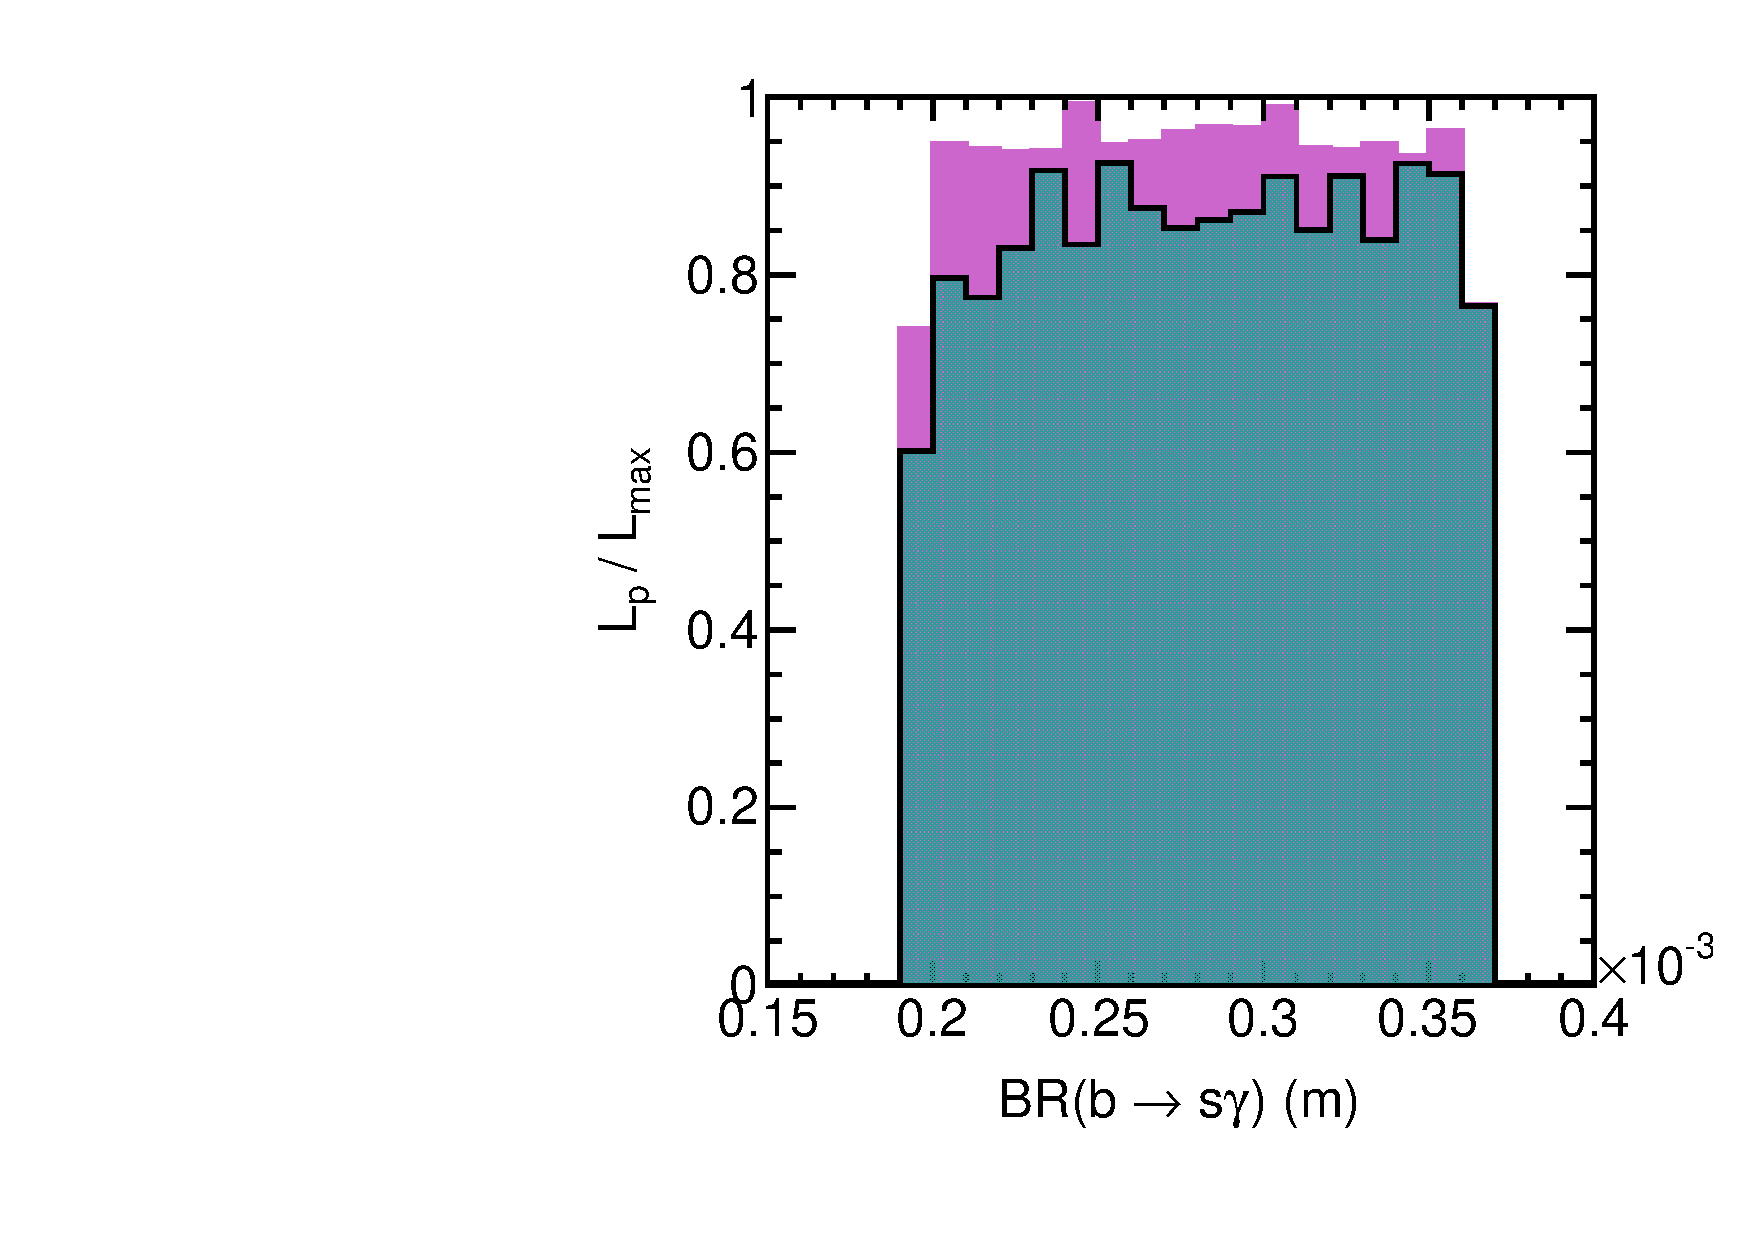
\includegraphics[height=5.5cm]{figs/fig_bsgamma_m.pdf} 
%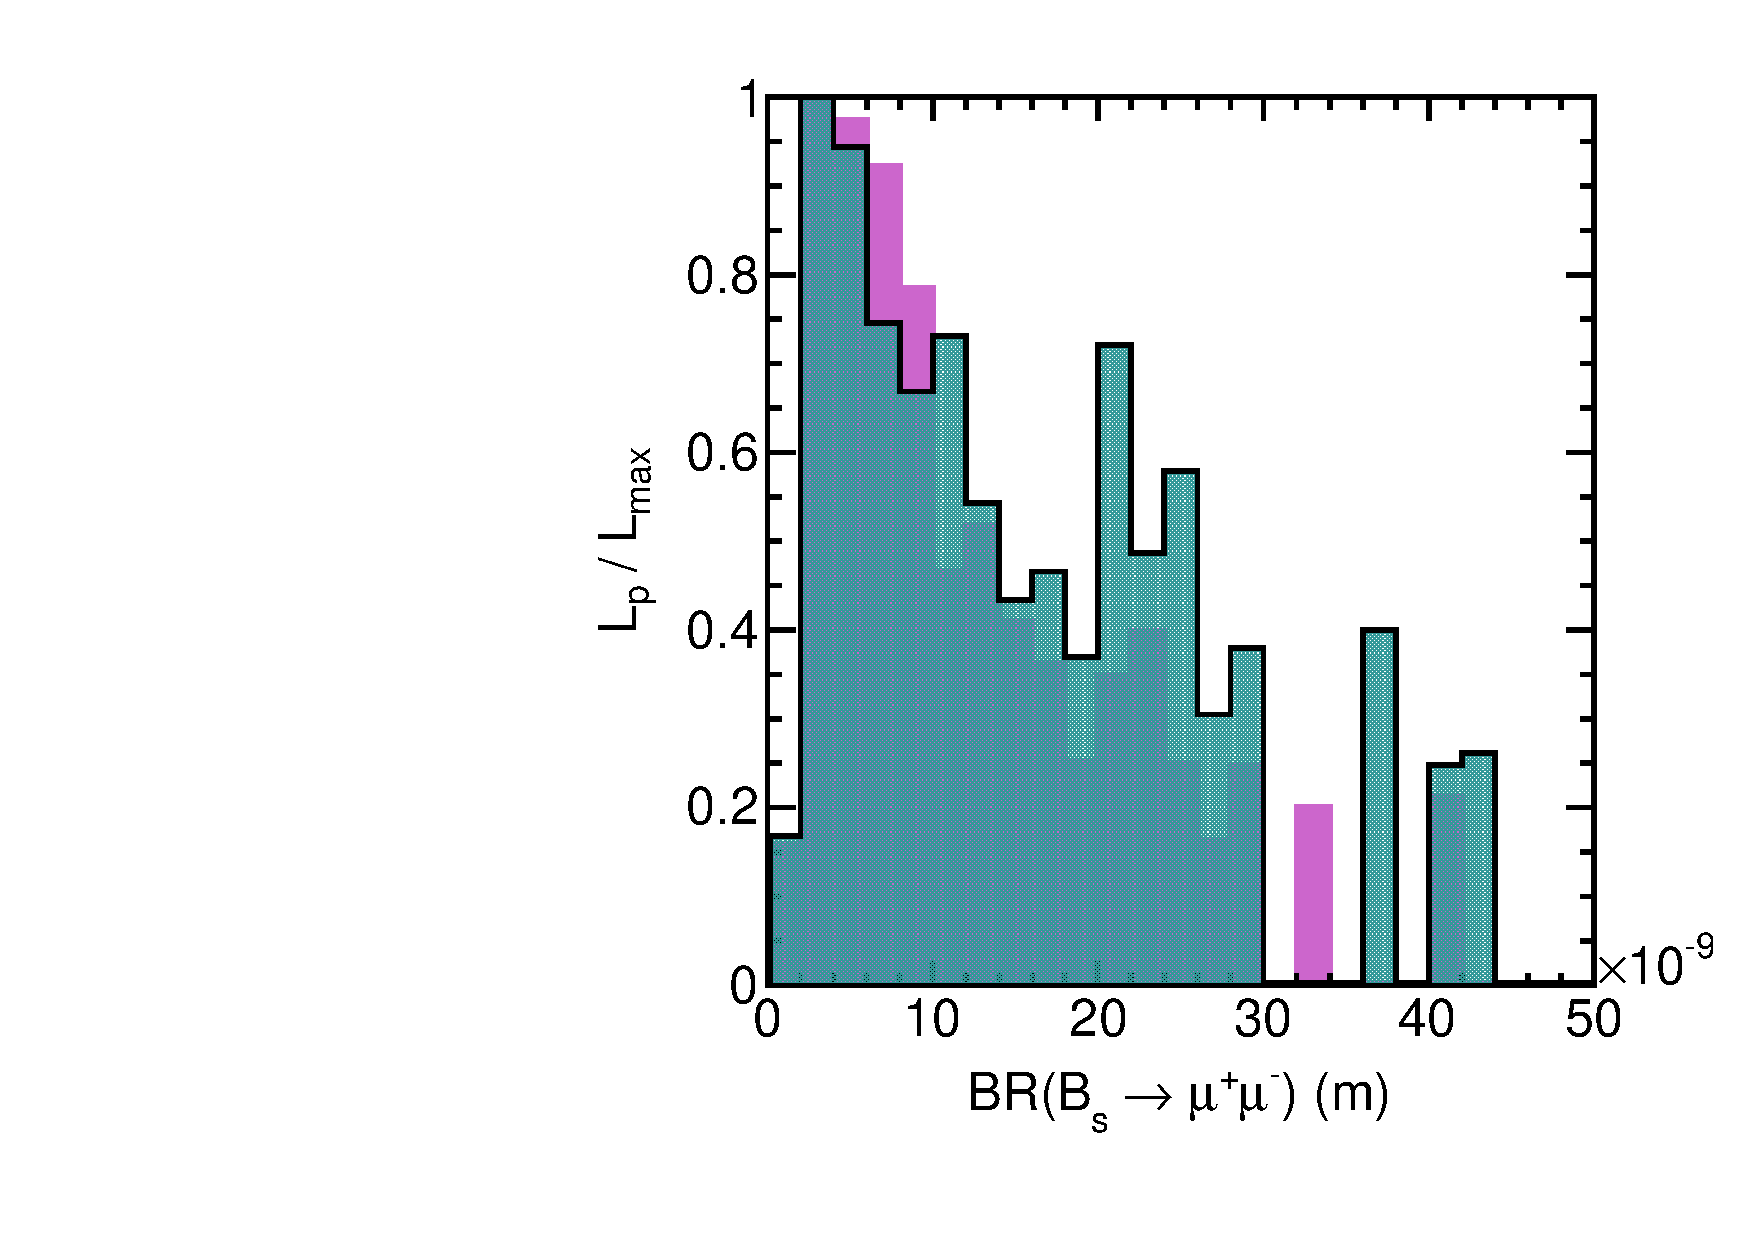
\includegraphics[height=5.5cm]{figs/fig_bsmumu_m.pdf} \\
%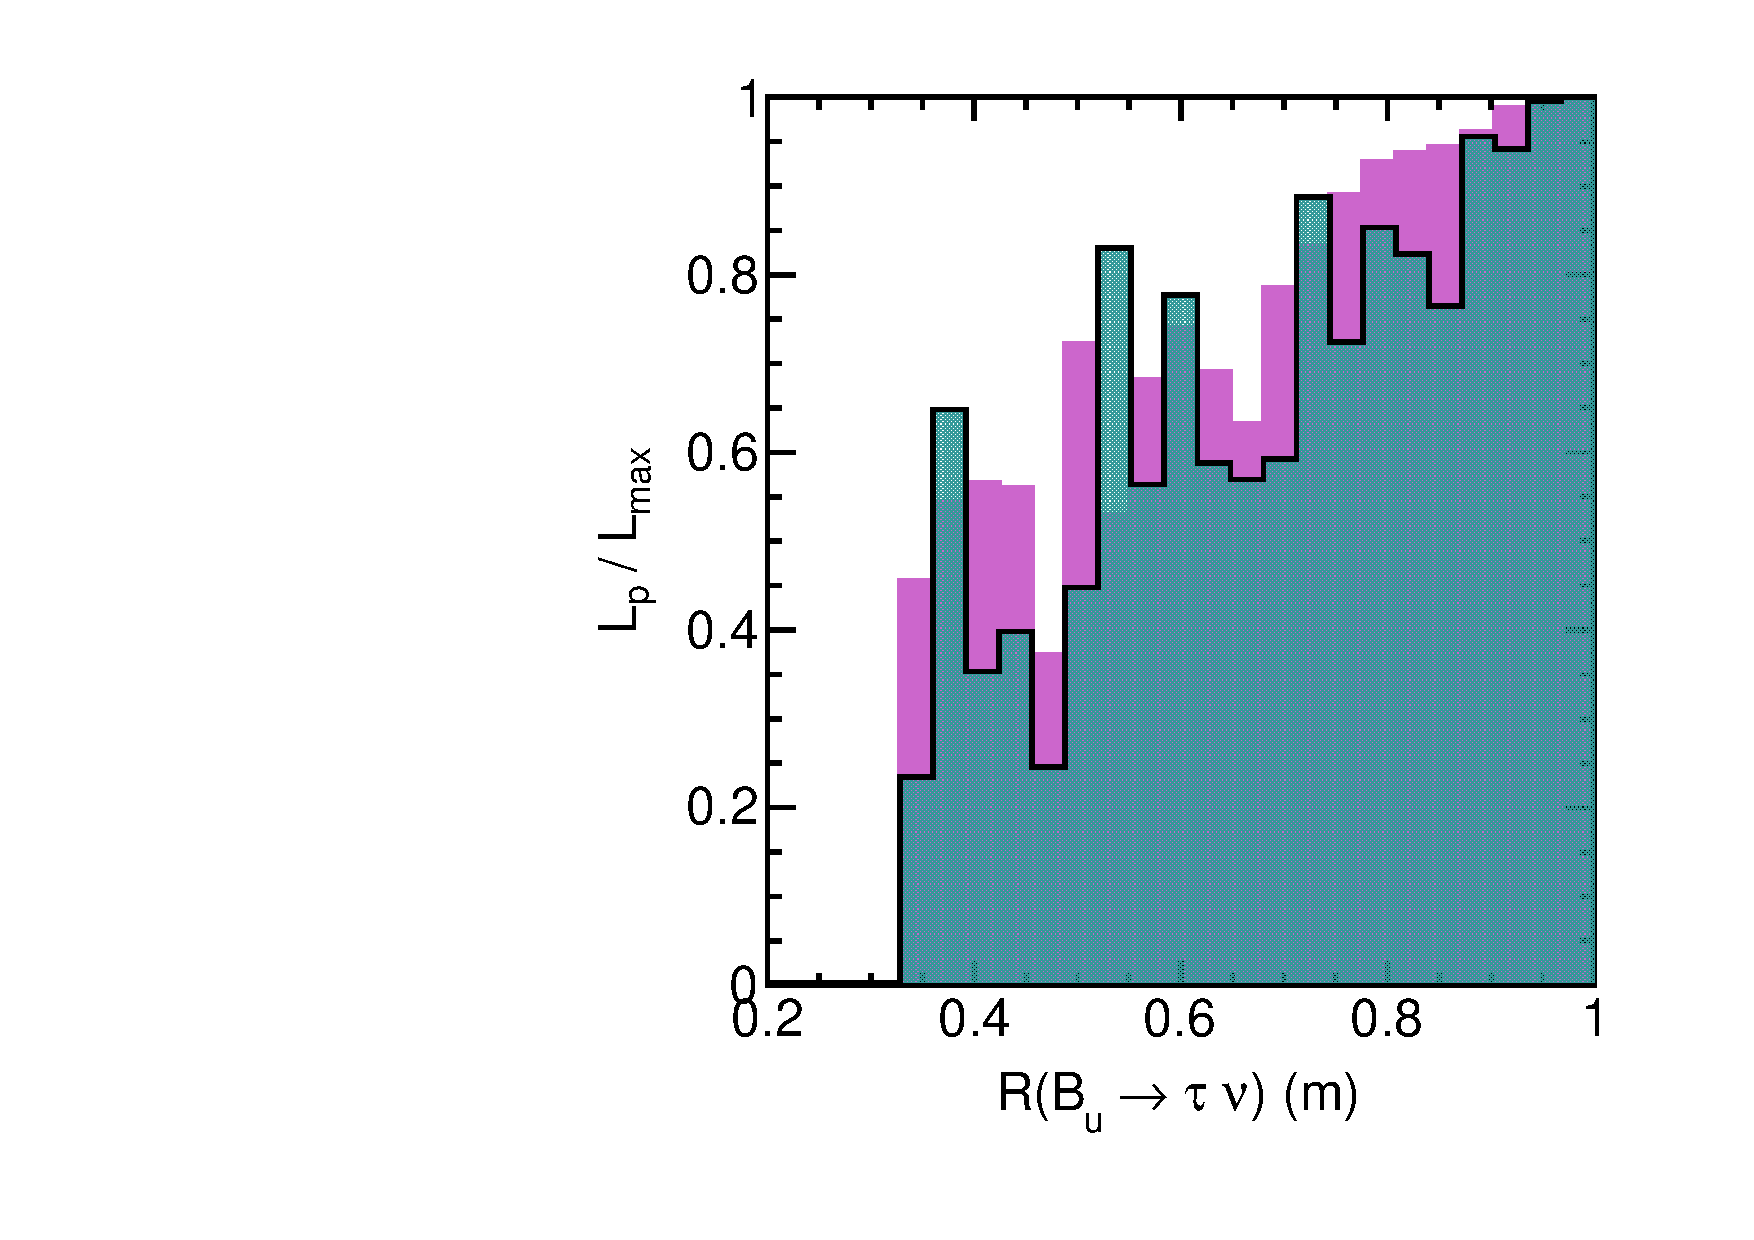
\includegraphics[height=5.5cm]{figs/fig_rbtaunu_m.pdf} 
%\caption{Ratios of profile likelihood $L_p$ to maximum likelihood $L_{max}$ shown for predictions for weak scale observables as calculated by micromegas.  The colored and shaded histograms show the distributions before and after the inclusion of the CMS results.}
%\label{fig:LRwcms_EWobs_m}
%\end{center}
%\end{figure}


\begin{figure}[htbp]
\begin{center}
%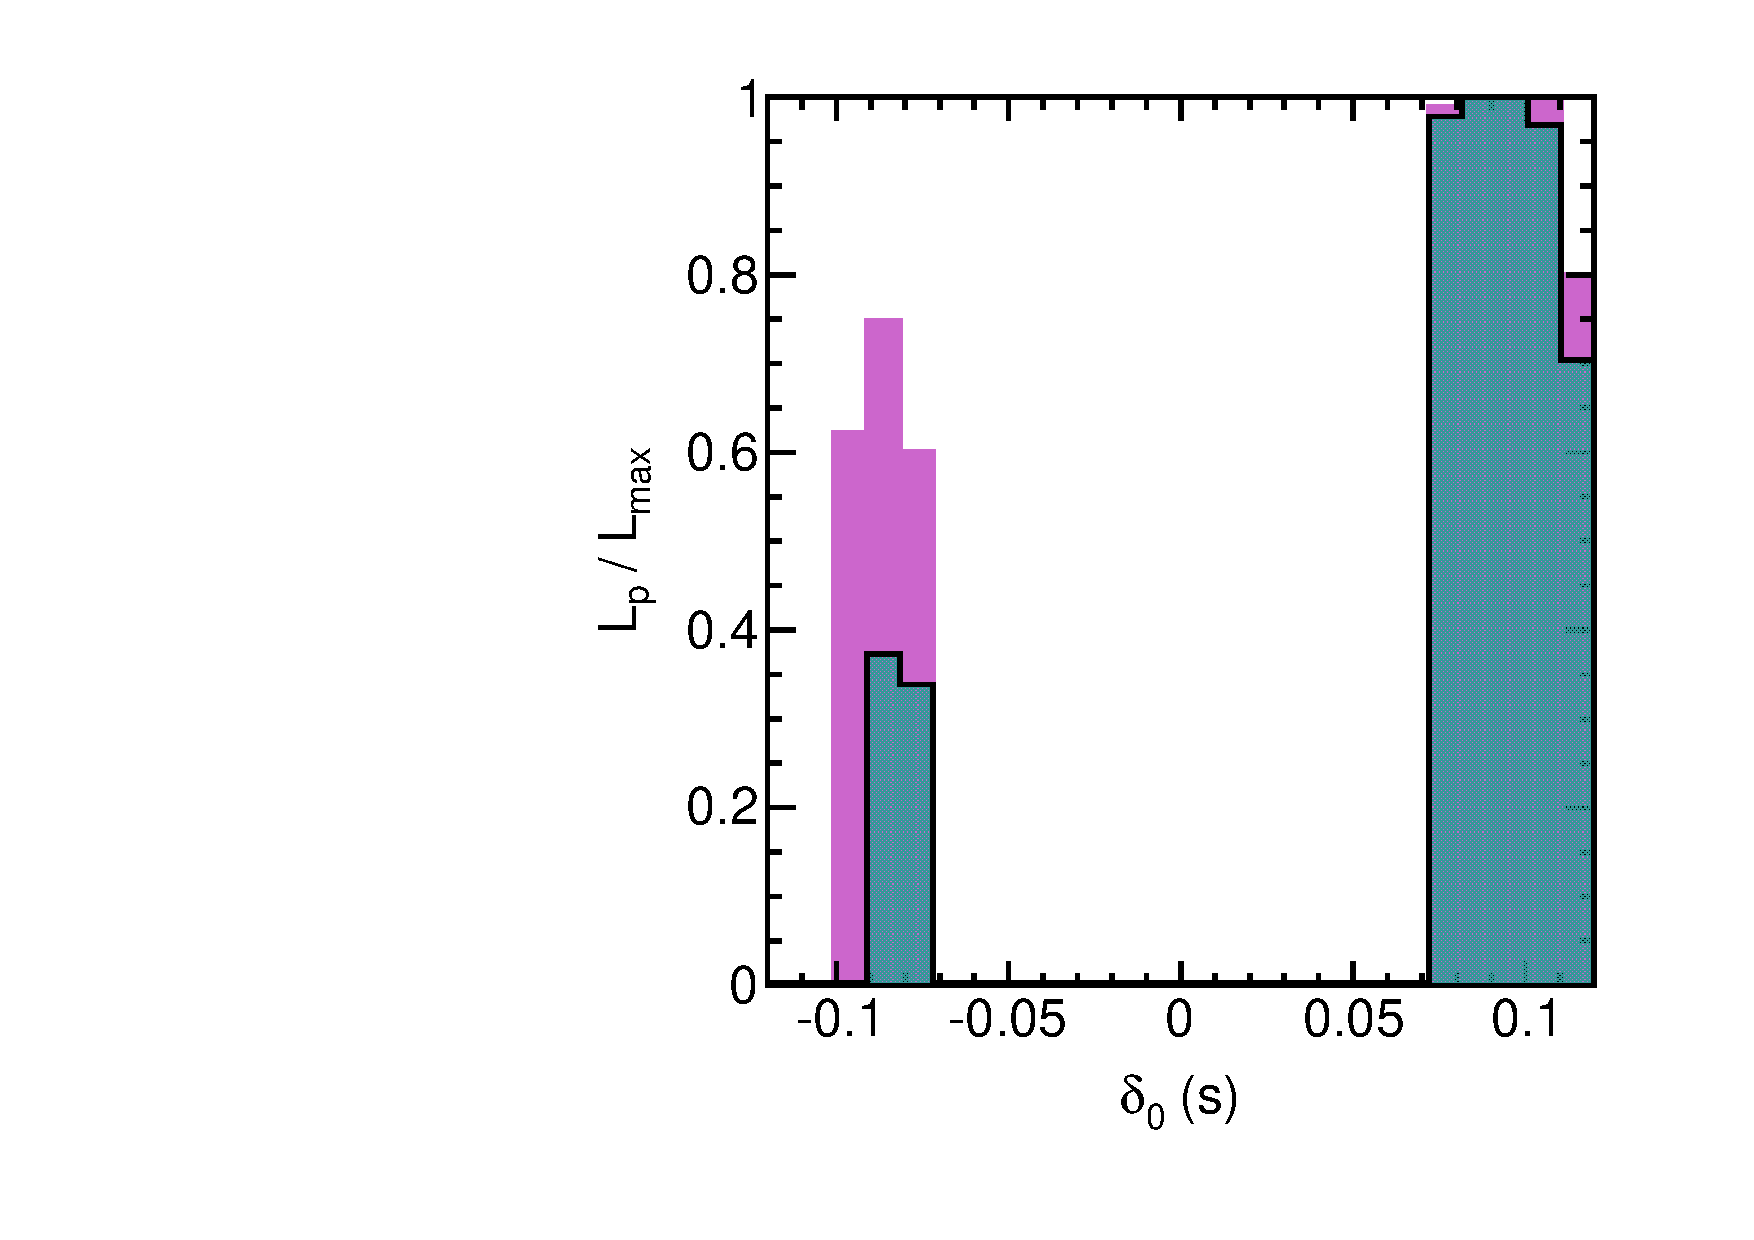
\includegraphics[height=5.5cm]{figs/fig_delta0_s.pdf} 
\includegraphics[height=5.5cm]{figs/fig_drho_m.pdf} 
\includegraphics[height=5.5cm]{figs/fig_muon_gm2_s.pdf} \\
\includegraphics[height=5.5cm]{figs/fig_bsgamma_s.pdf} 
\includegraphics[height=5.5cm]{figs/fig_Bsmumu_s.pdf} \\
\includegraphics[height=5.5cm]{figs/fig_Btaunu_s.pdf} 
\includegraphics[height=5.5cm]{figs/fig_RBtaunu_s.pdf} 
\caption{Ratios of profile likelihood $L_p$ to maximum likelihood $L_{max}$ shown for predictions for weak scale observables.  $\delta\rho$ is calculated using {\tt micrOMEGAs 2.4} and the rest are calculated using {\tt Superiso 2.7}.  The colored and shaded histograms show the distributions before and after the inclusion of the CMS results.}
\label{fig:LRwcms_EWobs_s1}
\end{center}
\end{figure}


\begin{figure}[htbp]
\begin{center}
\includegraphics[height=5.5cm]{figs/fig_BDtaunu_s.pdf} 
\includegraphics[height=5.5cm]{figs/fig_BDtaunu_BDenu_s.pdf} \\
\includegraphics[height=5.5cm]{figs/fig_Dmunu_s.pdf} 
\includegraphics[height=5.5cm]{figs/fig_Dsmunu_s.pdf} \\
\includegraphics[height=5.5cm]{figs/fig_Dstaunu_s.pdf} 
\includegraphics[height=5.5cm]{figs/fig_Kmunu_pimunu_s.pdf} \\
\includegraphics[height=5.5cm]{figs/fig_Rl23_s.pdf} 
\caption{Ratios of profile likelihood $L_p$ to maximum likelihood $L_{max}$ shown for predictions for weak scale observables as calculated by {\tt Superiso 2.7}.  The colored and shaded histograms show the distributions before and after the inclusion of the CMS results.}
\label{fig:LRwcms_EWobs_s2}
\end{center}
\end{figure}





